\chapter{Progettazione e implementazione dell'interfaccia utente}
\label{chap:design-implementation}

\section{Introduzione al capitolo}
Nel Capitolo~\ref{chap:digital-twin-smart-home} è stata descritta l'architettura complessiva del sistema e, in particolare, è stato evidenziato come la \textit{Digital Twin Interface} rappresenti il punto di contatto principale tra utente e Smart Home.

In questo capitolo viene descritto il lavoro di progettazione e sviluppo dell'interfaccia utente, partendo prima dal sistema di partenza e poi arrivando alle modifiche implementate durante questa tesi.

Le immagini presenti nella cartella \texttt{images/Chap - 4} rappresentano il sistema iniziale, mentre le immagini presenti in \texttt{images/Chap - 4/GOLINO} mostrano il mio sviluppo, incentrato soprattutto sulla creazione diretta delle automazioni TAP all'interno dell'interfaccia.

\section{Analisi del sistema di partenza}
\subsection{Panoramica generale dell'interfaccia}
Il sistema di partenza presenta una struttura generale coerente con quanto descritto nei capitoli precedenti: menu laterale persistente, sezioni principali ben separate e utilizzo della stessa identità visiva in tutte le schermate.

In particolare, le viste principali sono:
\begin{itemize}
    \item sezione \textbf{Consumption} per la visualizzazione dei consumi;
    \item sezione \textbf{Automations} per consultare e attivare/disattivare le routine;
    \item sezione \textbf{Configuration} per la configurazione iniziale e successiva della casa;
    \item area \textbf{Profile} per preferenze utente, consensi privacy e dati personali.
\end{itemize}

Una vista complessiva della sezione consumi è mostrata in (fig.~\ref{fig:cap4_base_consumptions_overview}).

\begin{figure}[H]
    \centering
    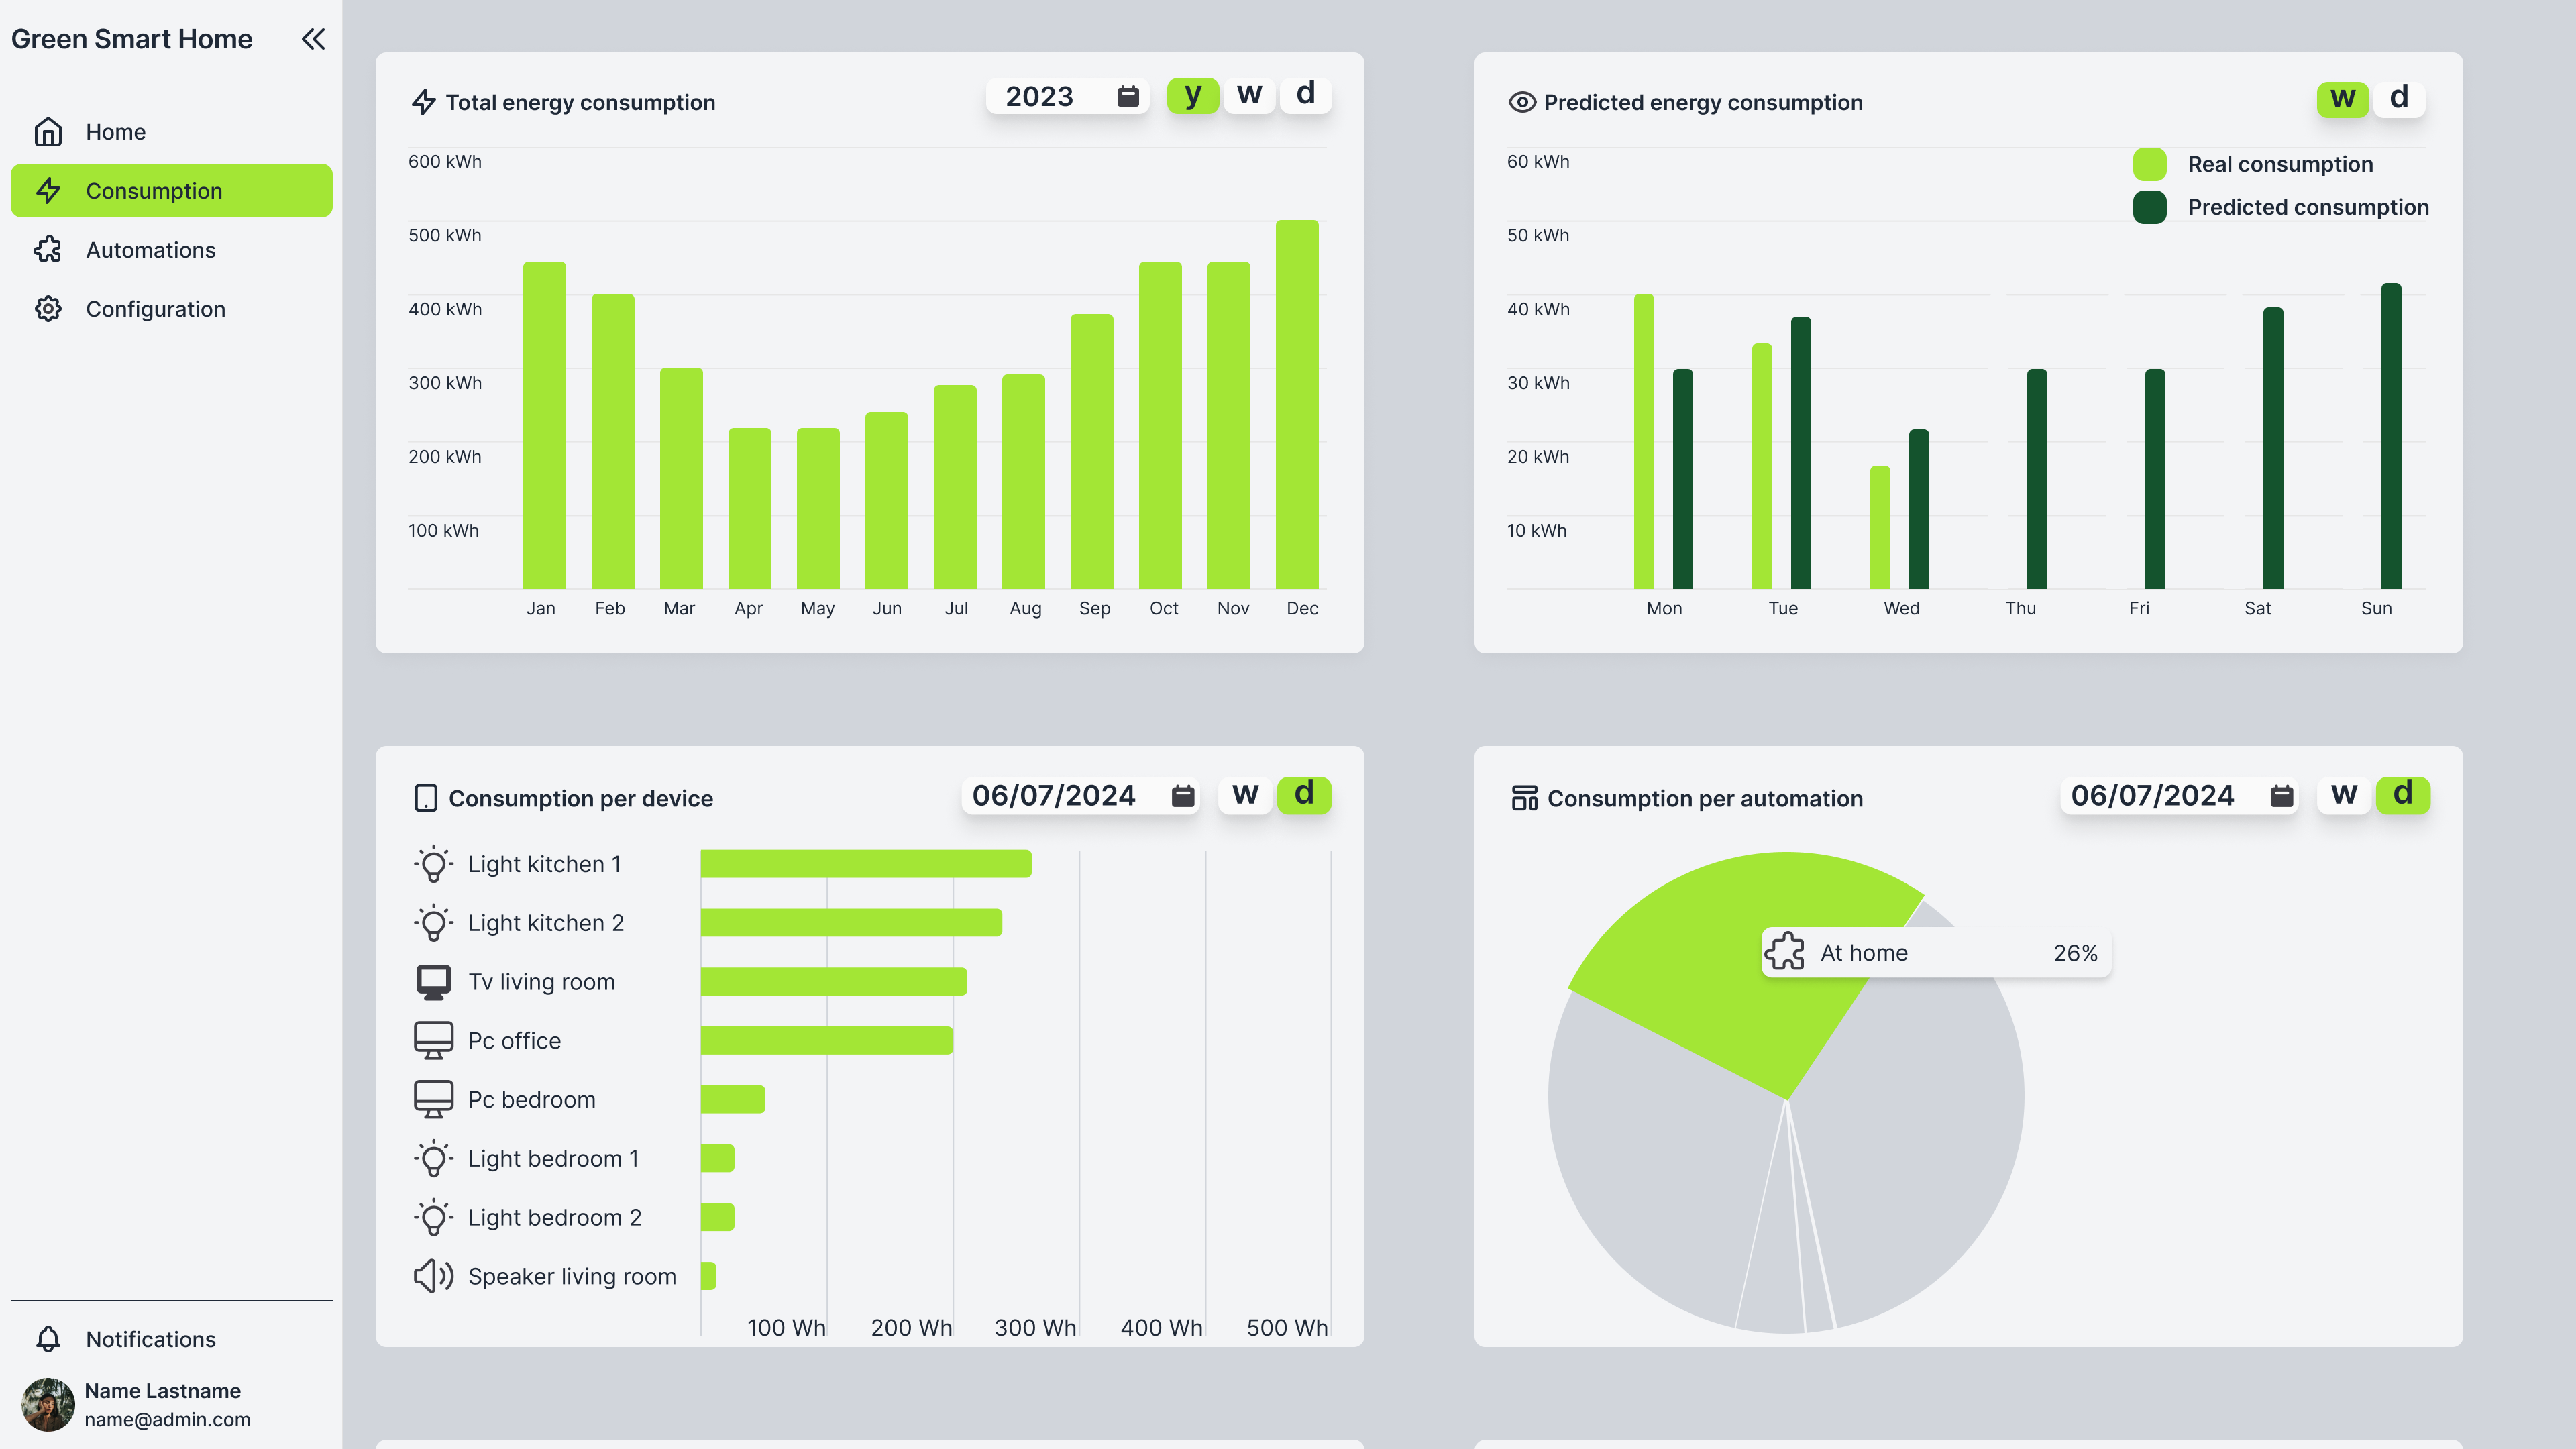
\includegraphics[width=1\linewidth]{images/Chap - 4/Consumptions.png}
    \caption{Sistema di partenza: vista generale della sezione consumi}
    \label{fig:cap4_base_consumptions_overview}
\end{figure}

La schermata delle automazioni, riportata in (fig.~\ref{fig:cap4_base_automations}), consente la gestione delle routine già presenti, la consultazione dello stato e la visualizzazione di suggerimenti energetici.

\begin{figure}[H]
    \centering
    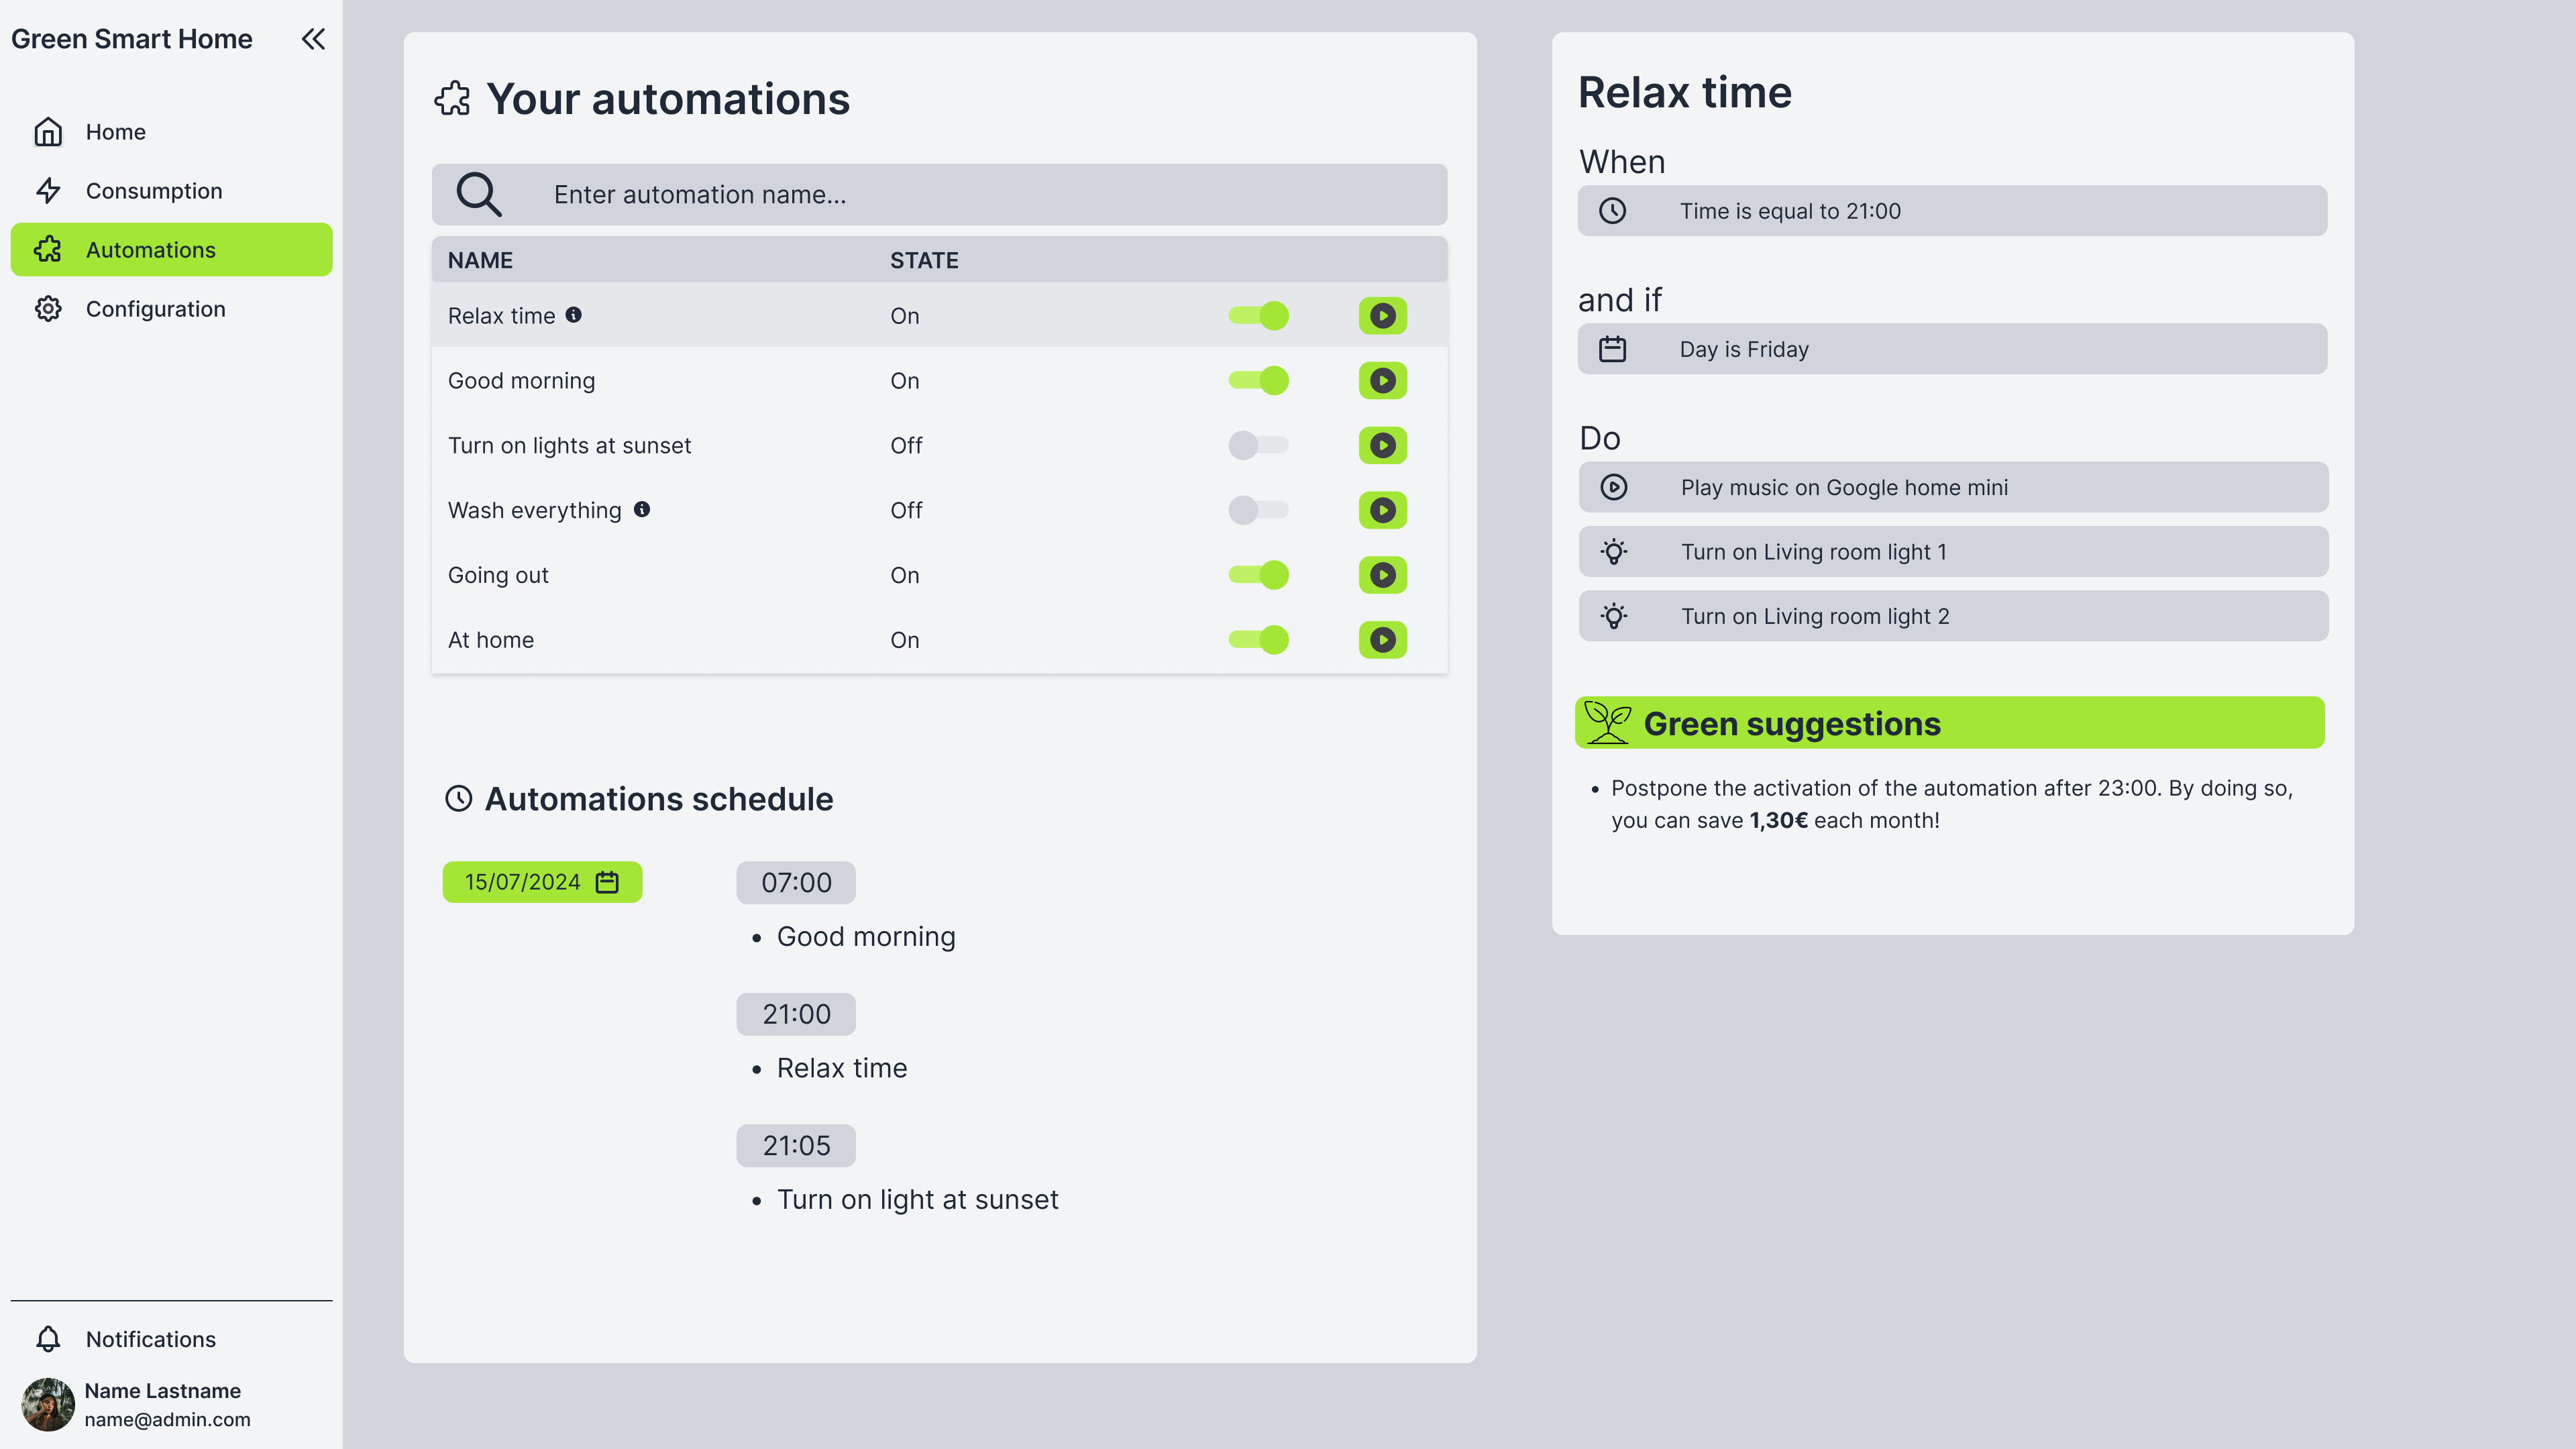
\includegraphics[width=1\linewidth]{images/Chap - 4/Automations.png}
    \caption{Sistema di partenza: sezione automazioni}
    \label{fig:cap4_base_automations}
\end{figure}

La parte destra della sezione automazioni mostra il dettaglio della routine selezionata, con blocchi \textit{When}, \textit{and if}, \textit{Do} e i suggerimenti green. Un esempio focalizzato di questo blocco è riportato in (fig.~\ref{fig:cap4_base_automation_detail}).

\begin{figure}[H]
    \centering
    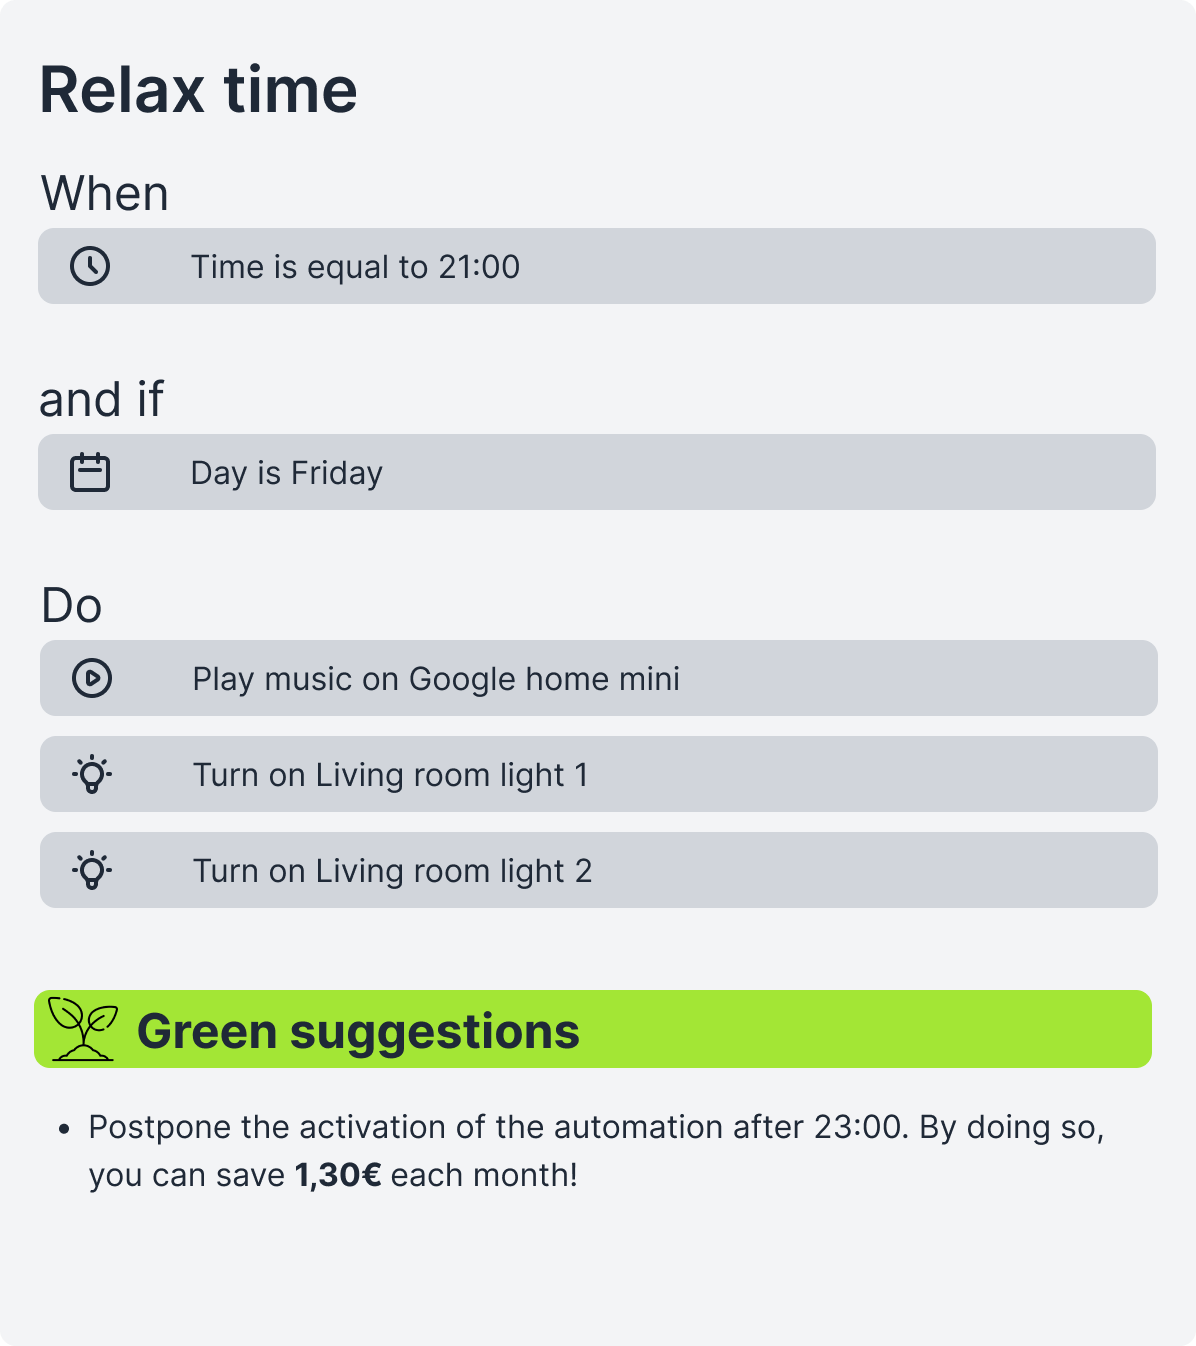
\includegraphics[width=0.6\linewidth]{images/Chap - 4/Frame 2610521.png}
    \caption{Sistema di partenza: dettaglio di una automazione con suggerimenti}
    \label{fig:cap4_base_automation_detail}
\end{figure}

\subsection{Analisi della sezione consumi}
La sezione consumi nel sistema di partenza è una delle parti più complete dell'interfaccia. L'utente può cambiare \textit{timespan} (giorno, settimana, anno), scegliere modalità diverse (consumo totale, per dispositivo, per automazione, predizione, ecc.) e alternare il tipo di grafico.

Una vista giornaliera del consumo totale corrente è mostrata in (fig.~\ref{fig:cap4_base_total_day_current}), mentre in (fig.~\ref{fig:cap4_base_total_day_past}) è visibile lo stesso grafico su una data passata.

\begin{figure}[H]
    \centering
    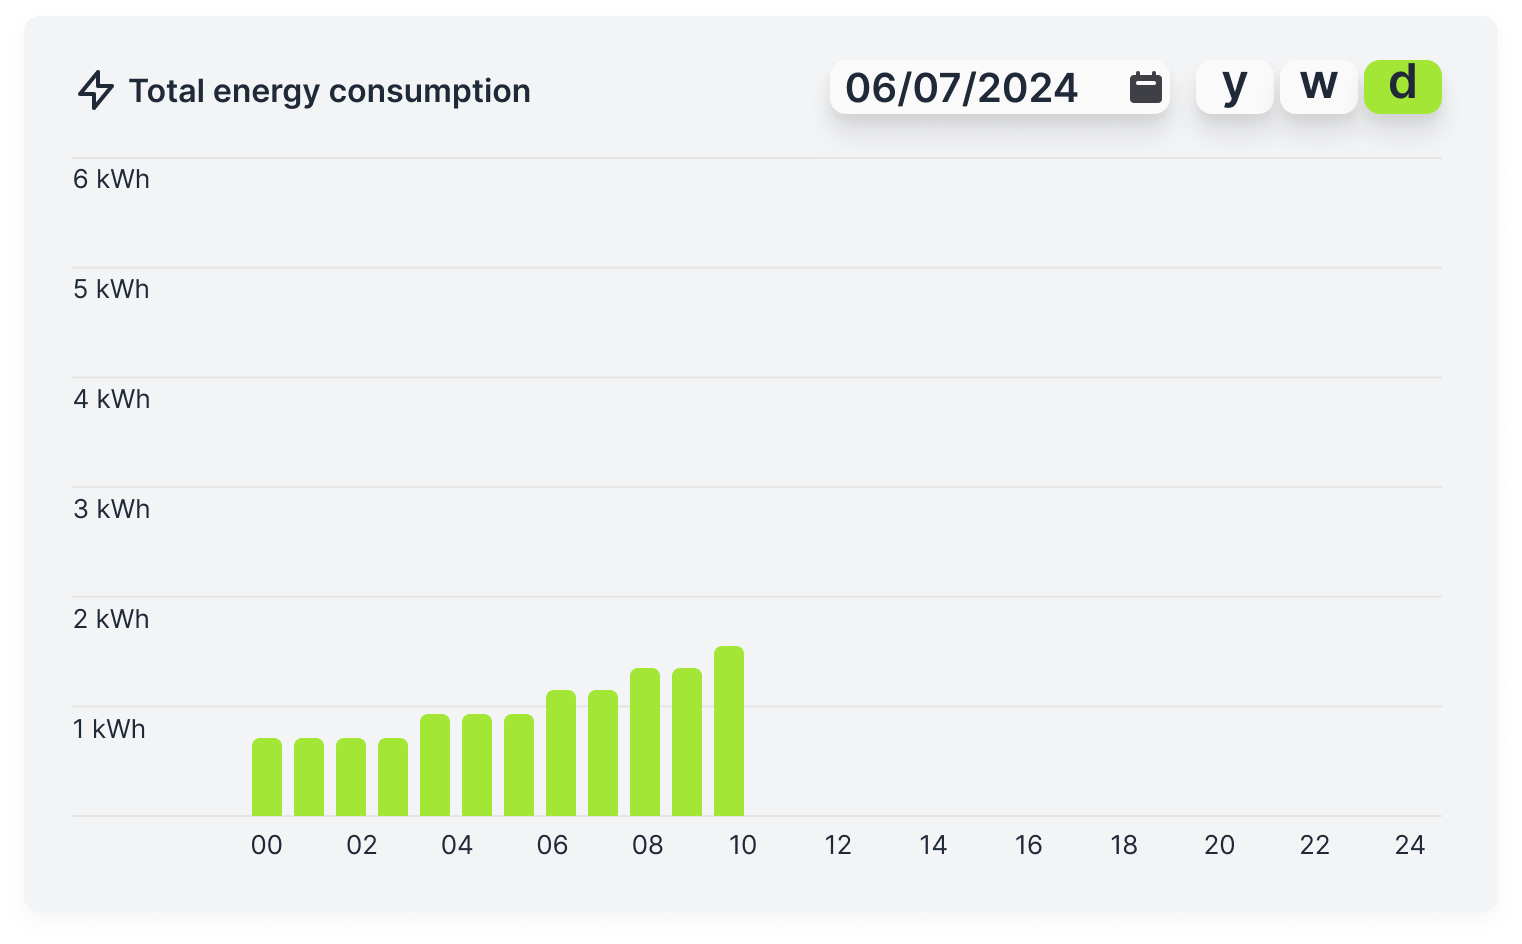
\includegraphics[width=0.95\linewidth]{images/Chap - 4/Timespan=Day, Mode=Total energy, Graph=Bar, Date=Current.png}
    \caption{Sistema di partenza: consumo totale giornaliero (data corrente)}
    \label{fig:cap4_base_total_day_current}
\end{figure}

\begin{figure}[H]
    \centering
    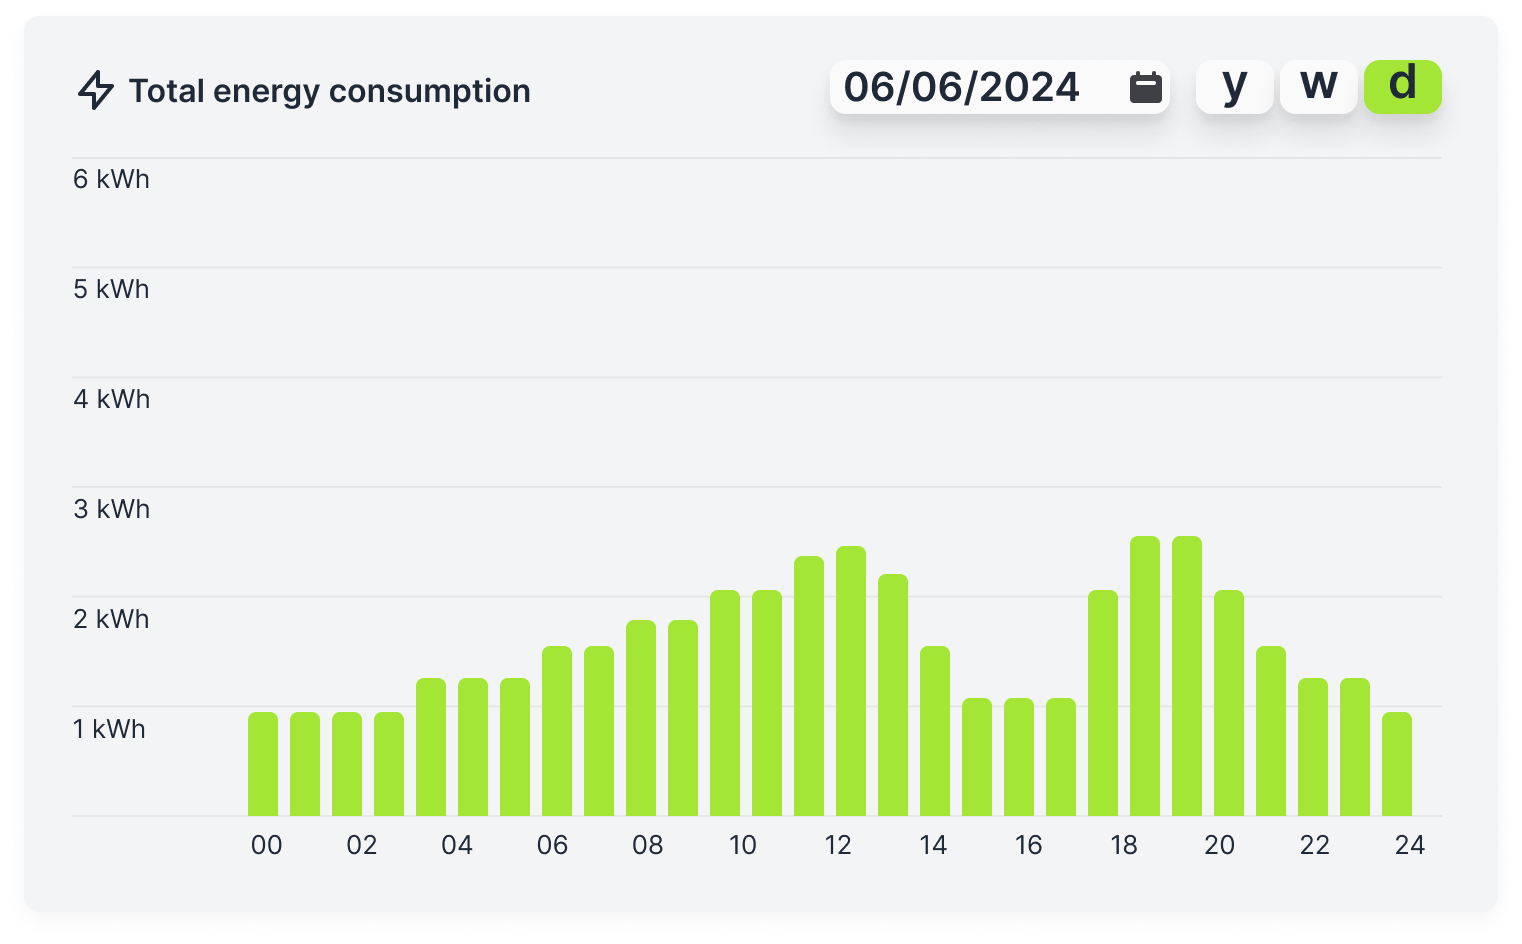
\includegraphics[width=0.95\linewidth]{images/Chap - 4/Timespan=Day, Mode=Total energy, Graph=Bar, Date=Past.png}
    \caption{Sistema di partenza: consumo totale giornaliero (data passata)}
    \label{fig:cap4_base_total_day_past}
\end{figure}

Lo stesso approccio è presente anche per l'intervallo settimanale. In (fig.~\ref{fig:cap4_base_total_week_current}) è mostrata la settimana corrente, mentre in (fig.~\ref{fig:cap4_base_total_week_past}) una settimana passata.

\begin{figure}[H]
    \centering
    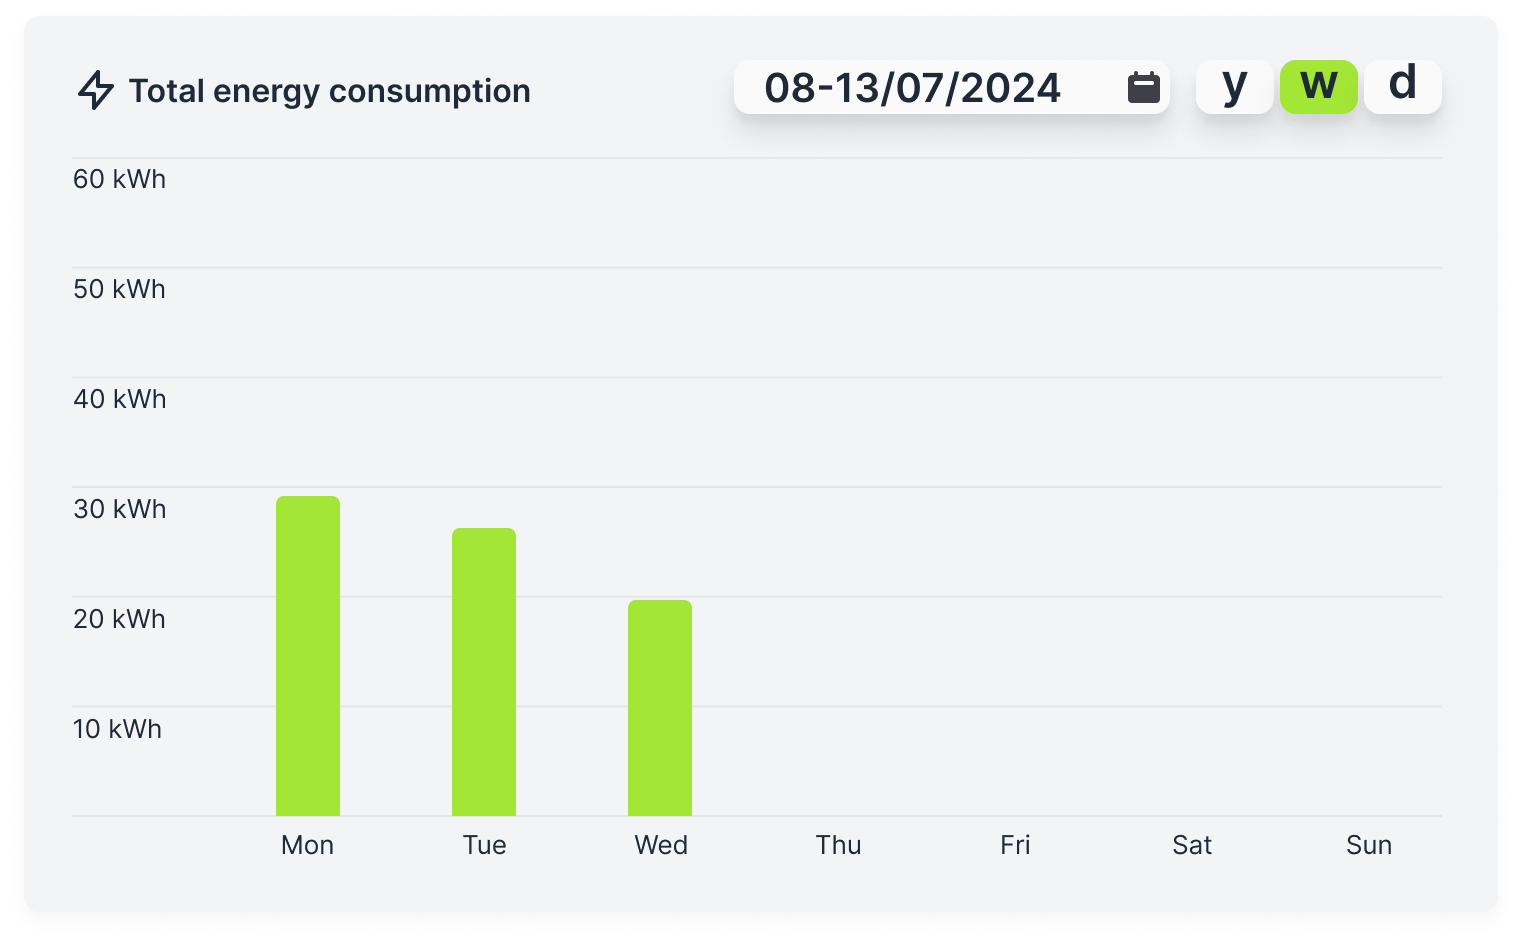
\includegraphics[width=0.95\linewidth]{images/Chap - 4/Timespan=Week, Mode=Total energy, Graph=Bar, Date=Current.png}
    \caption{Sistema di partenza: consumo totale settimanale (corrente)}
    \label{fig:cap4_base_total_week_current}
\end{figure}

\begin{figure}[H]
    \centering
    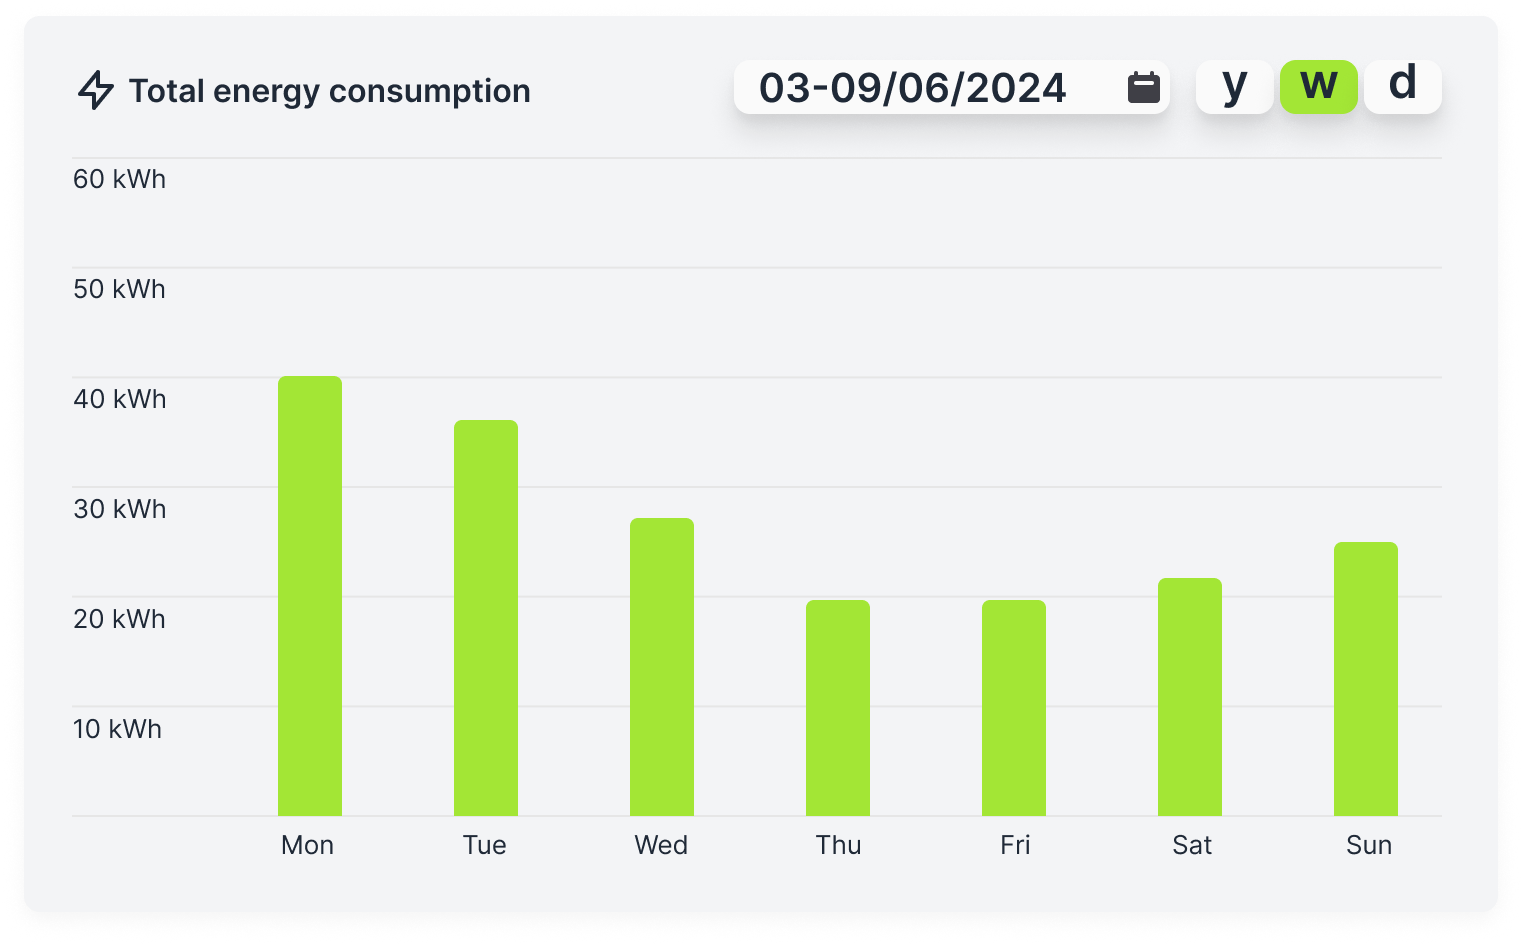
\includegraphics[width=0.95\linewidth]{images/Chap - 4/Timespan=Week, Mode=Total energy, Graph=Bar, Date=Past.png}
    \caption{Sistema di partenza: consumo totale settimanale (passato)}
    \label{fig:cap4_base_total_week_past}
\end{figure}

Per la scala annuale, il sistema permette di confrontare anni differenti, come mostrato in (fig.~\ref{fig:cap4_base_total_year_current}) e (fig.~\ref{fig:cap4_base_total_year_past}).

\begin{figure}[H]
    \centering
    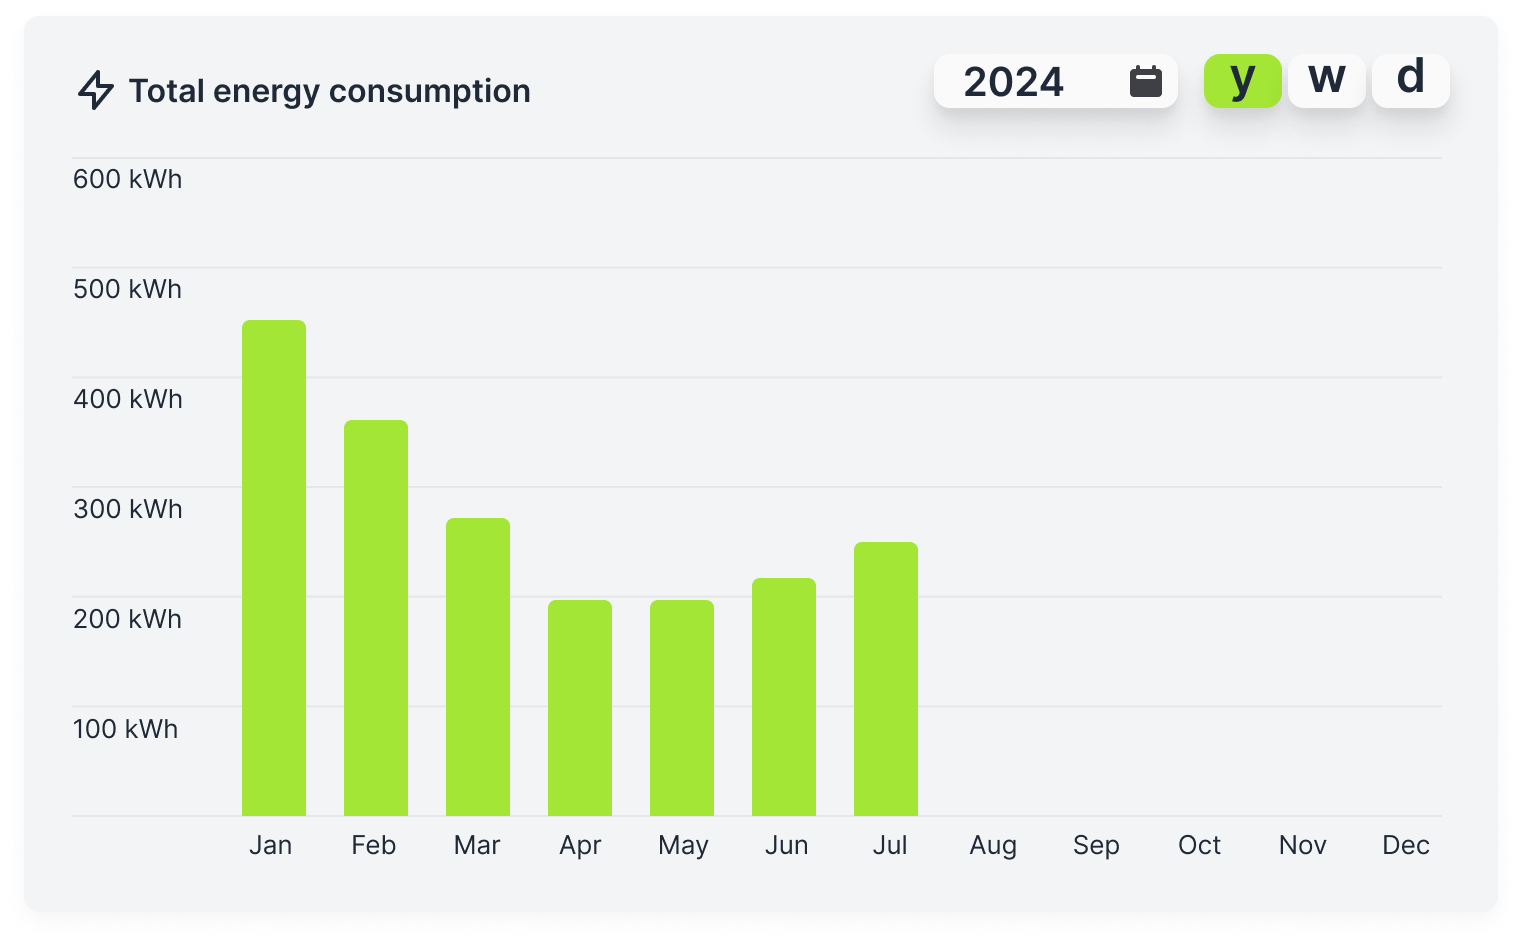
\includegraphics[width=0.95\linewidth]{images/Chap - 4/Timespan=Year, Mode=Total energy, Graph=Bar, Date=Current.png}
    \caption{Sistema di partenza: consumo totale annuale (anno corrente)}
    \label{fig:cap4_base_total_year_current}
\end{figure}

\begin{figure}[H]
    \centering
    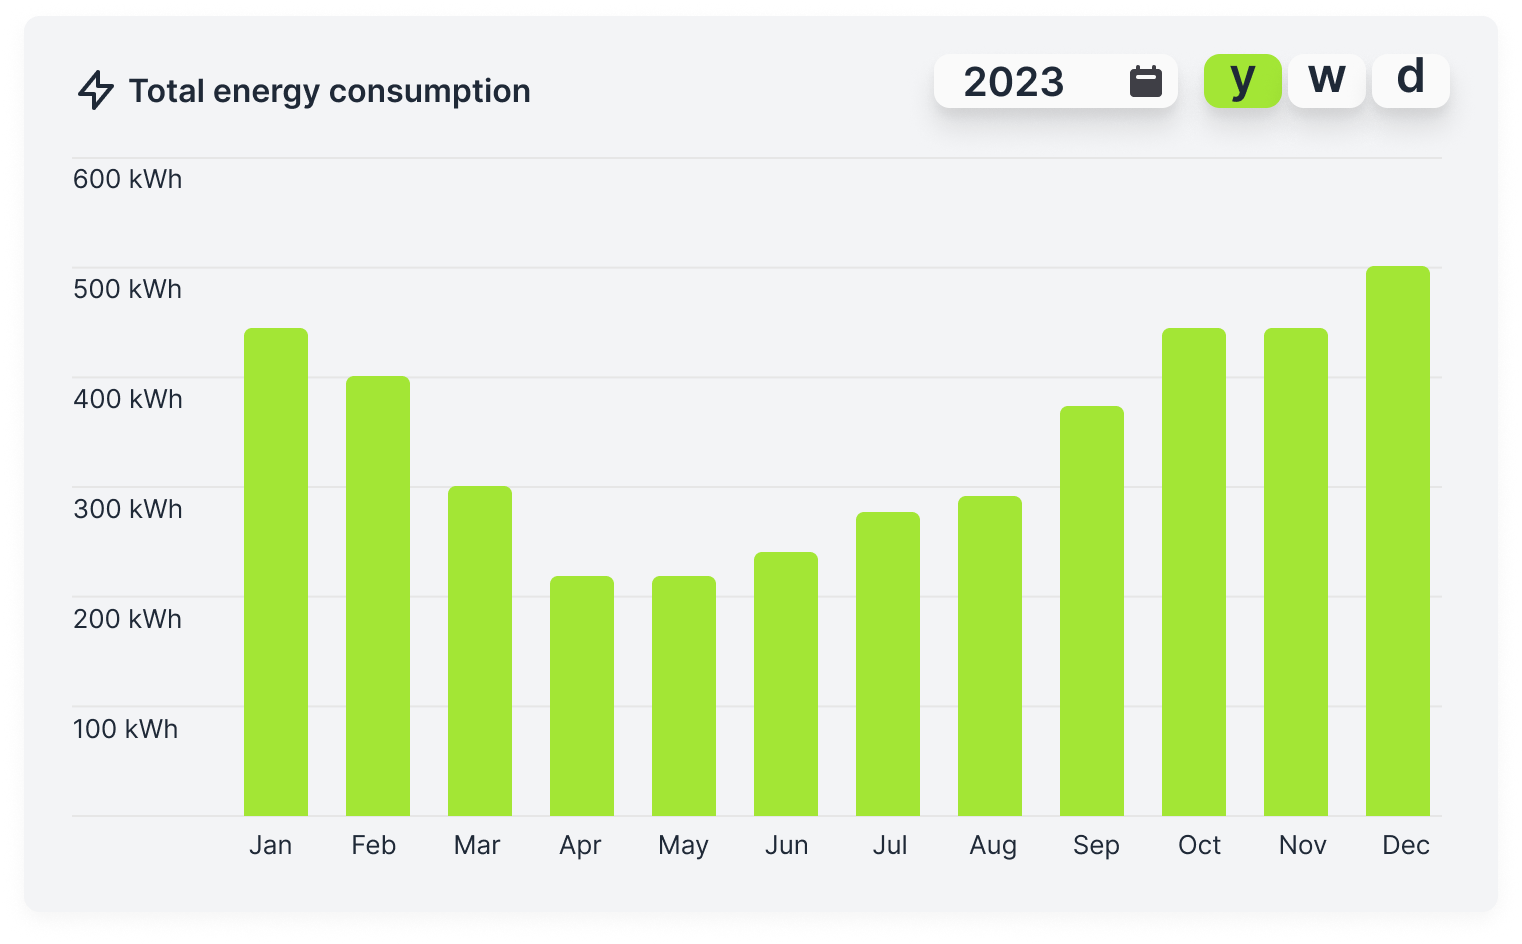
\includegraphics[width=0.95\linewidth]{images/Chap - 4/Timespan=Year, Mode=Total energy, Graph=Bar, Date=Past.png}
    \caption{Sistema di partenza: consumo totale annuale (anno passato)}
    \label{fig:cap4_base_total_year_past}
\end{figure}

La parte predittiva è mostrata sia in versione barre-linea (fig.~\ref{fig:cap4_base_pred_day_line}) sia in versione settimanale con confronto tra consumo reale e predetto (fig.~\ref{fig:cap4_base_pred_week}).

\begin{figure}[H]
    \centering
    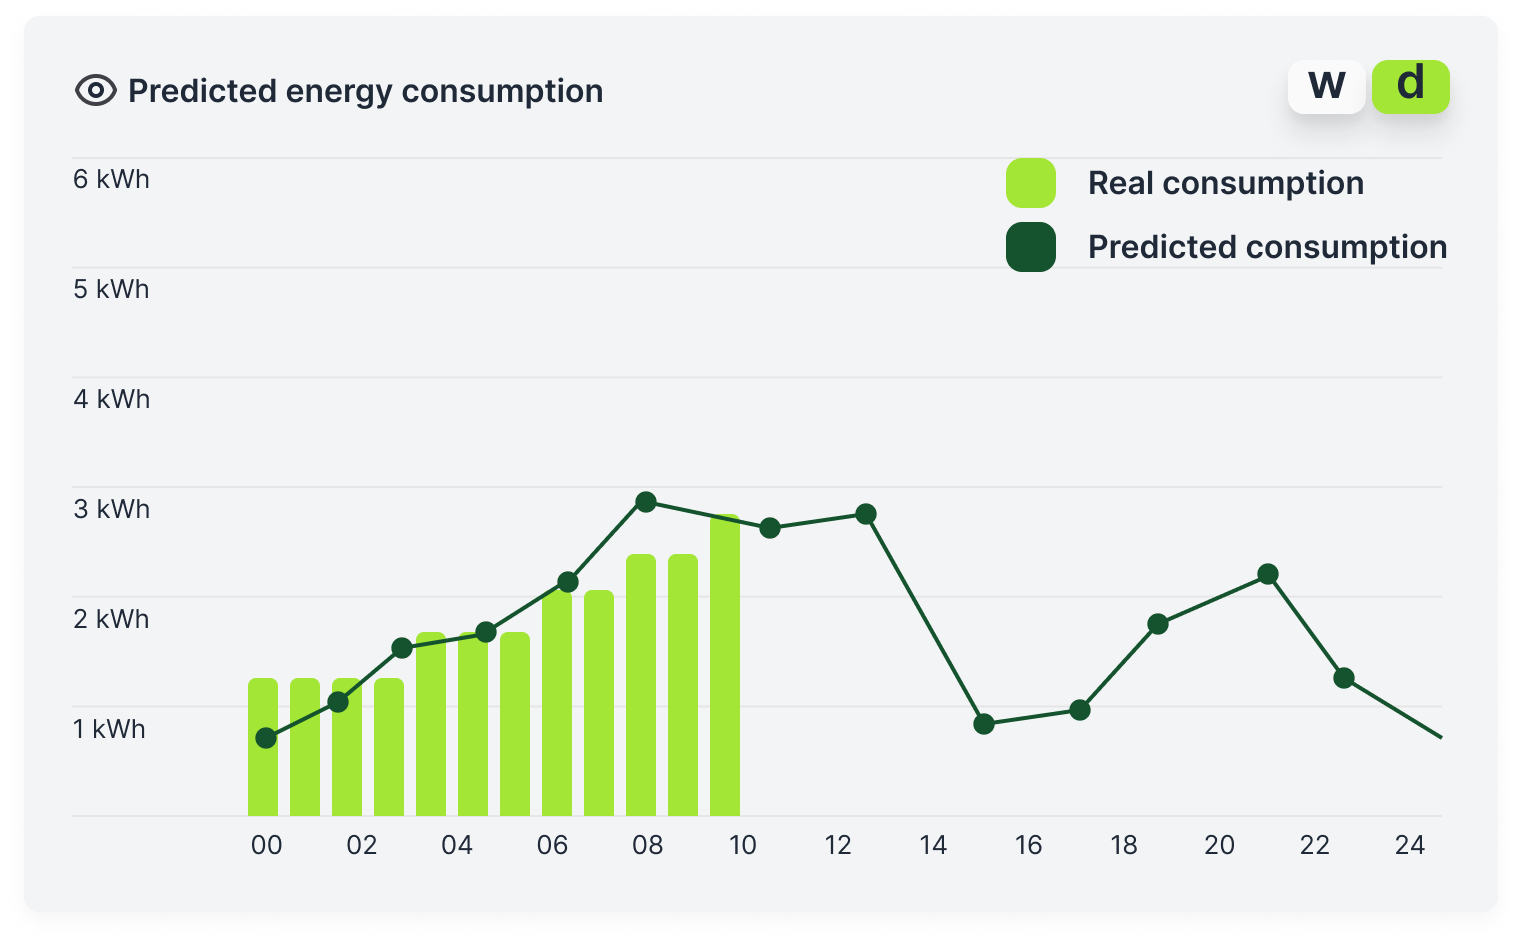
\includegraphics[width=0.95\linewidth]{images/Chap - 4/Timespan=Day, Mode=Predicted energy, Graph=Bar-Line, Date=Current.png}
    \caption{Sistema di partenza: consumo predetto giornaliero (barre + linea)}
    \label{fig:cap4_base_pred_day_line}
\end{figure}

\begin{figure}[H]
    \centering
    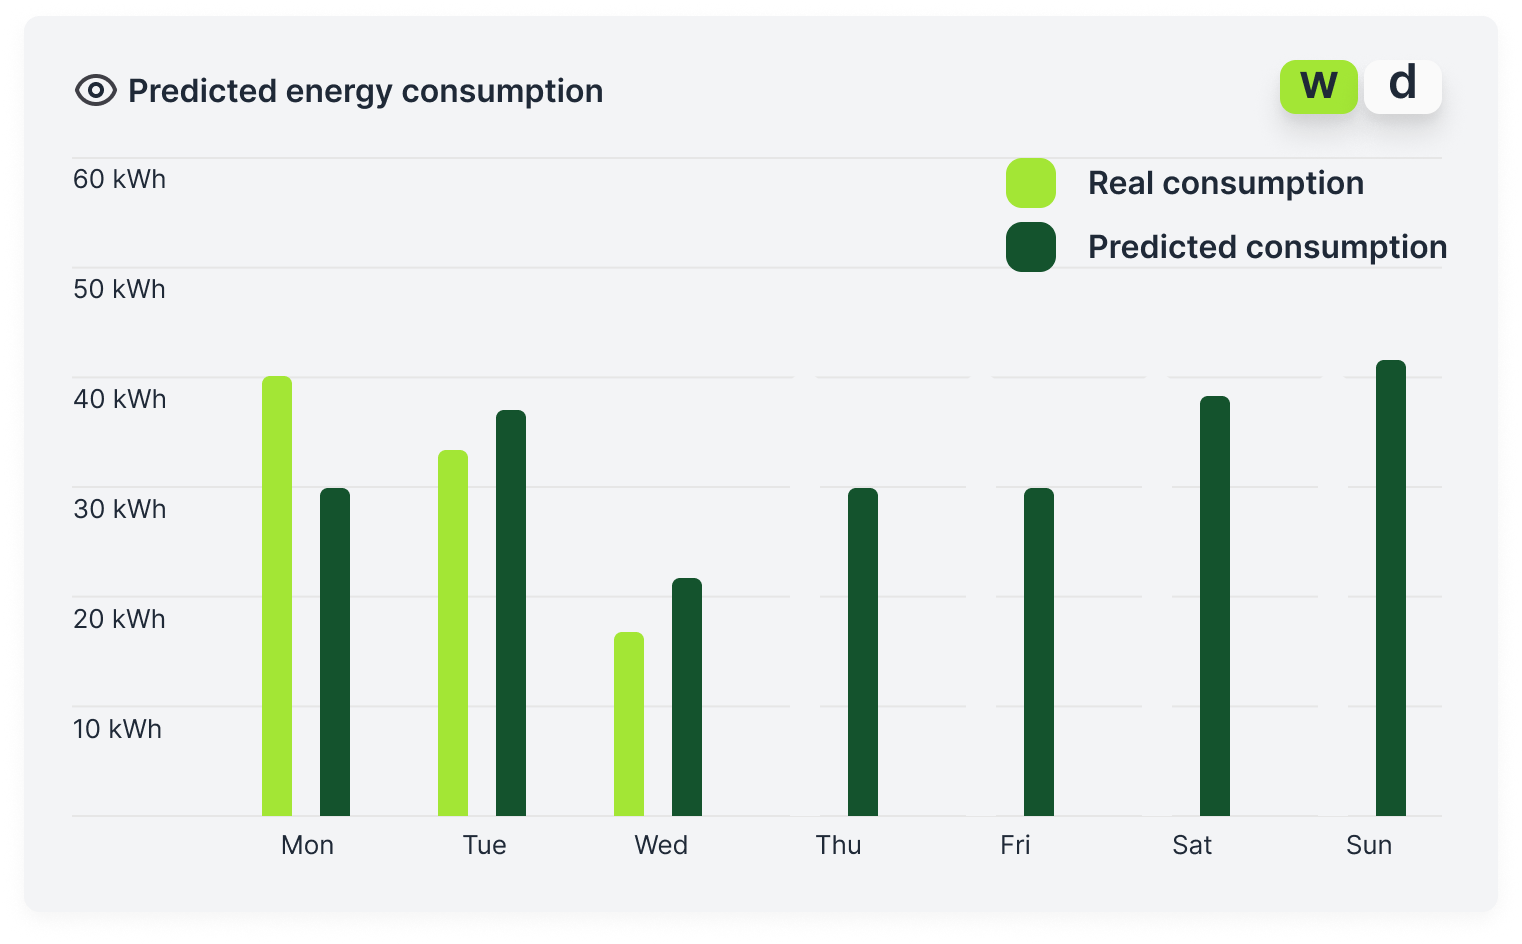
\includegraphics[width=0.95\linewidth]{images/Chap - 4/Timespan=Week, Mode=Predicted energy, Graph=Bar, Date=Current.png}
    \caption{Sistema di partenza: consumo predetto settimanale}
    \label{fig:cap4_base_pred_week}
\end{figure}

Oltre al consumo totale, il sistema permette anche analisi per dispositivo e per automazione, sia a barre sia a torta, come riportato in (fig.~\ref{fig:cap4_base_device_bar}), (fig.~\ref{fig:cap4_base_device_pie}), (fig.~\ref{fig:cap4_base_automation_bar}) e (fig.~\ref{fig:cap4_base_automation_pie}).

\begin{figure}[H]
    \centering
    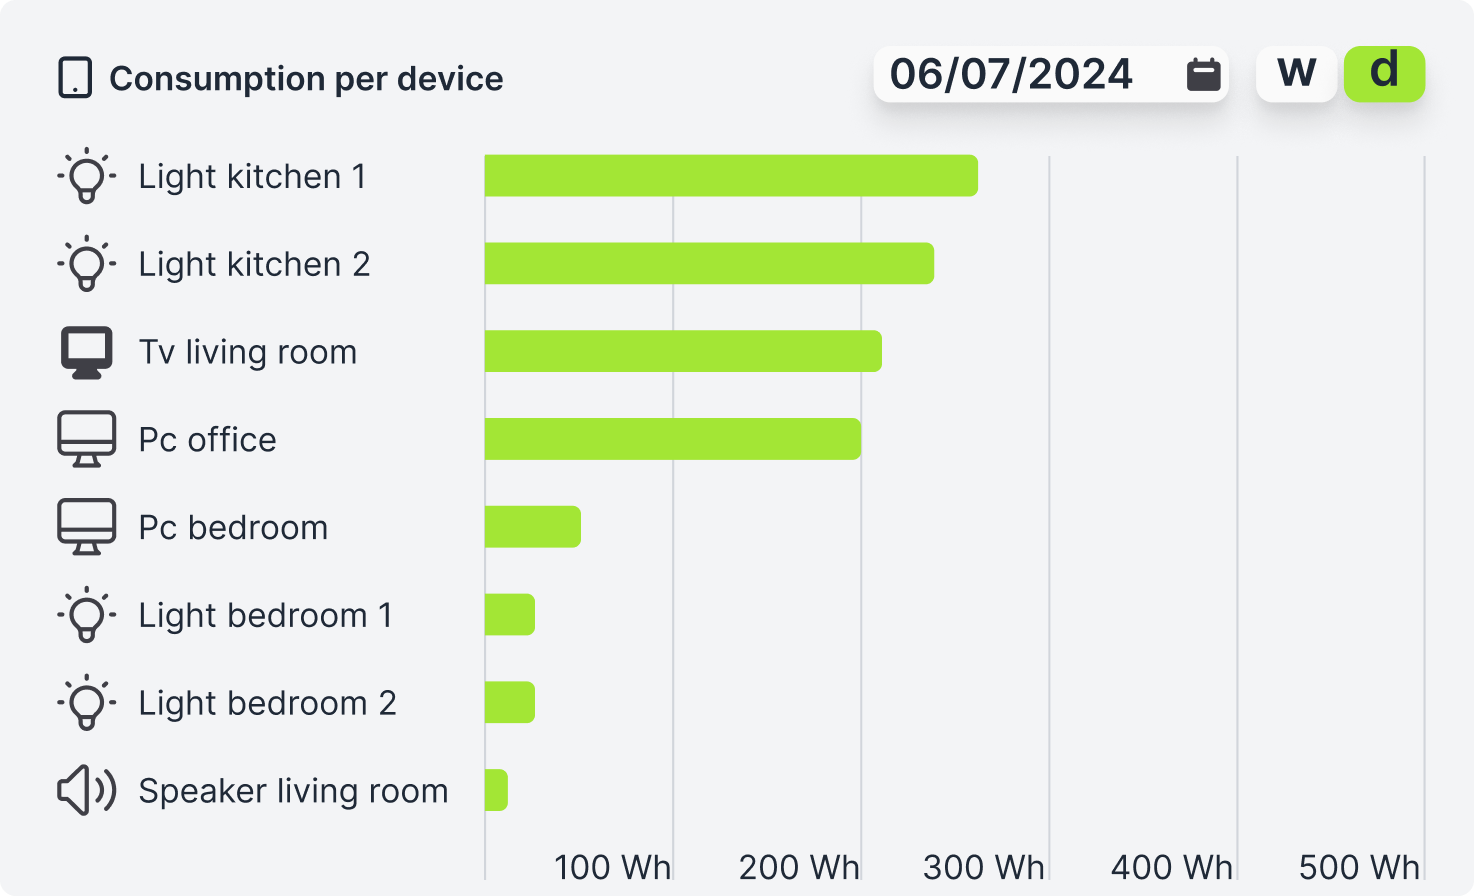
\includegraphics[width=0.95\linewidth]{images/Chap - 4/Timespan=Day, Mode=Appliance energy, Graph=Bar, Date=Past.png}
    \caption{Sistema di partenza: consumo per dispositivo (barre)}
    \label{fig:cap4_base_device_bar}
\end{figure}

\begin{figure}[H]
    \centering
    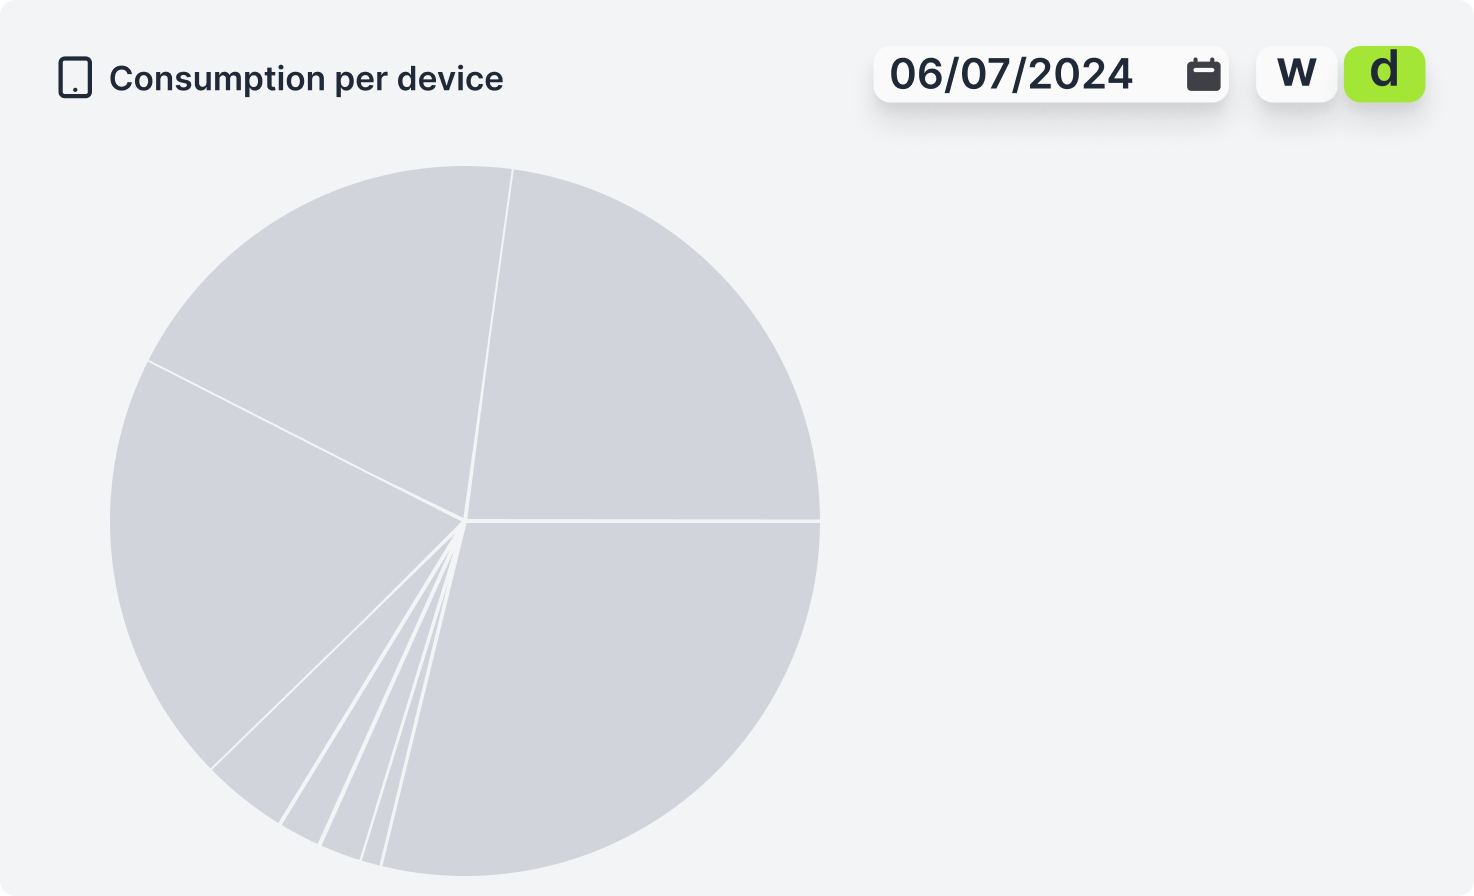
\includegraphics[width=0.95\linewidth]{images/Chap - 4/Timespan=Day, Mode=Appliance energy, Graph=Pie, Date=Past.png}
    \caption{Sistema di partenza: consumo per dispositivo (torta)}
    \label{fig:cap4_base_device_pie}
\end{figure}

\begin{figure}[H]
    \centering
    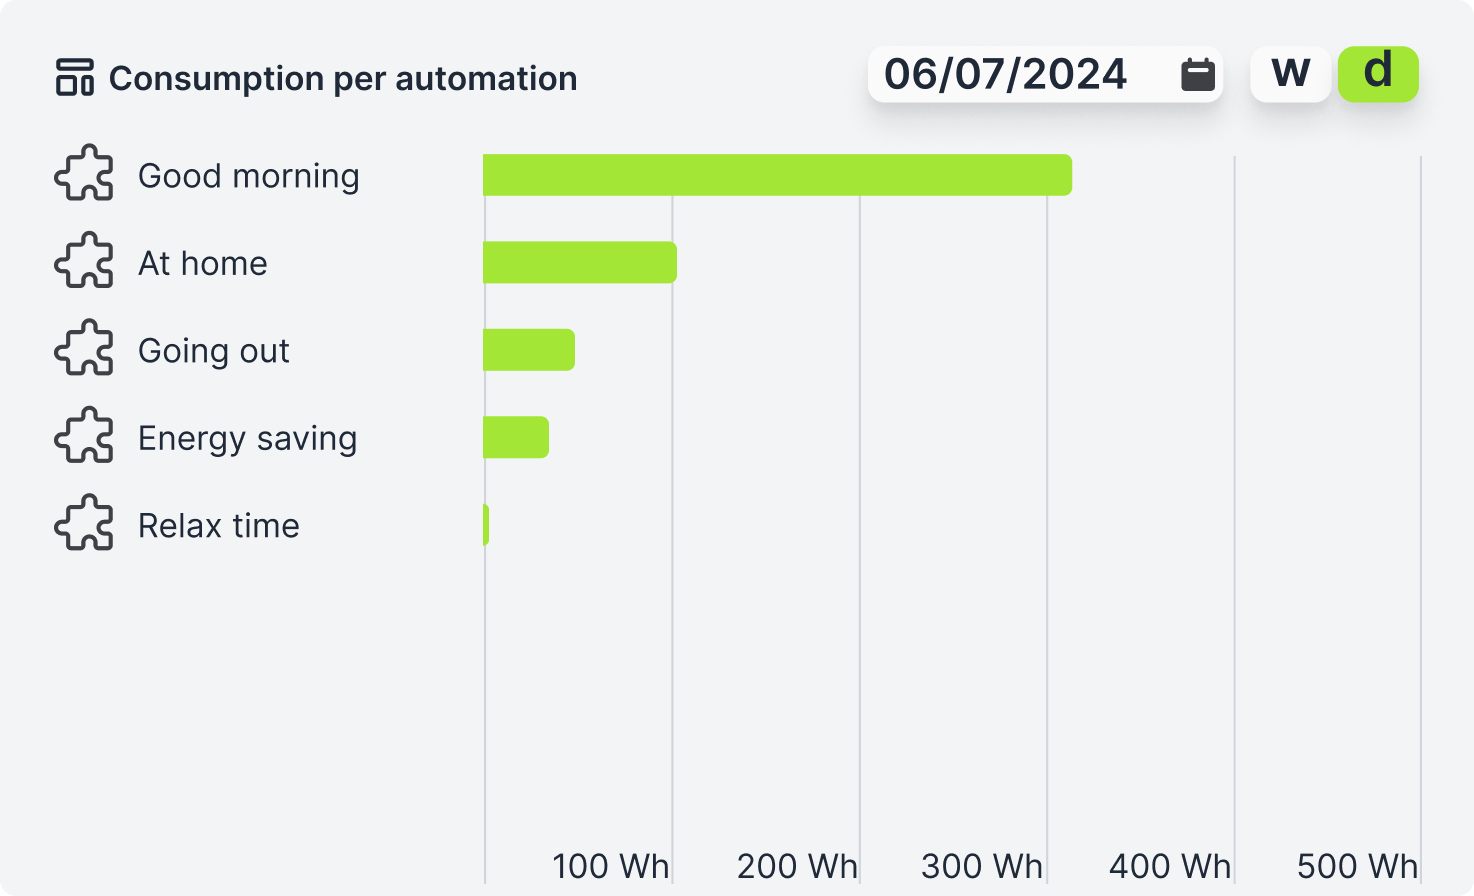
\includegraphics[width=0.95\linewidth]{images/Chap - 4/Timespan=Day, Mode=Automation energy, Graph=Bar, Date=Past.png}
    \caption{Sistema di partenza: consumo per automazione (barre)}
    \label{fig:cap4_base_automation_bar}
\end{figure}

\begin{figure}[H]
    \centering
    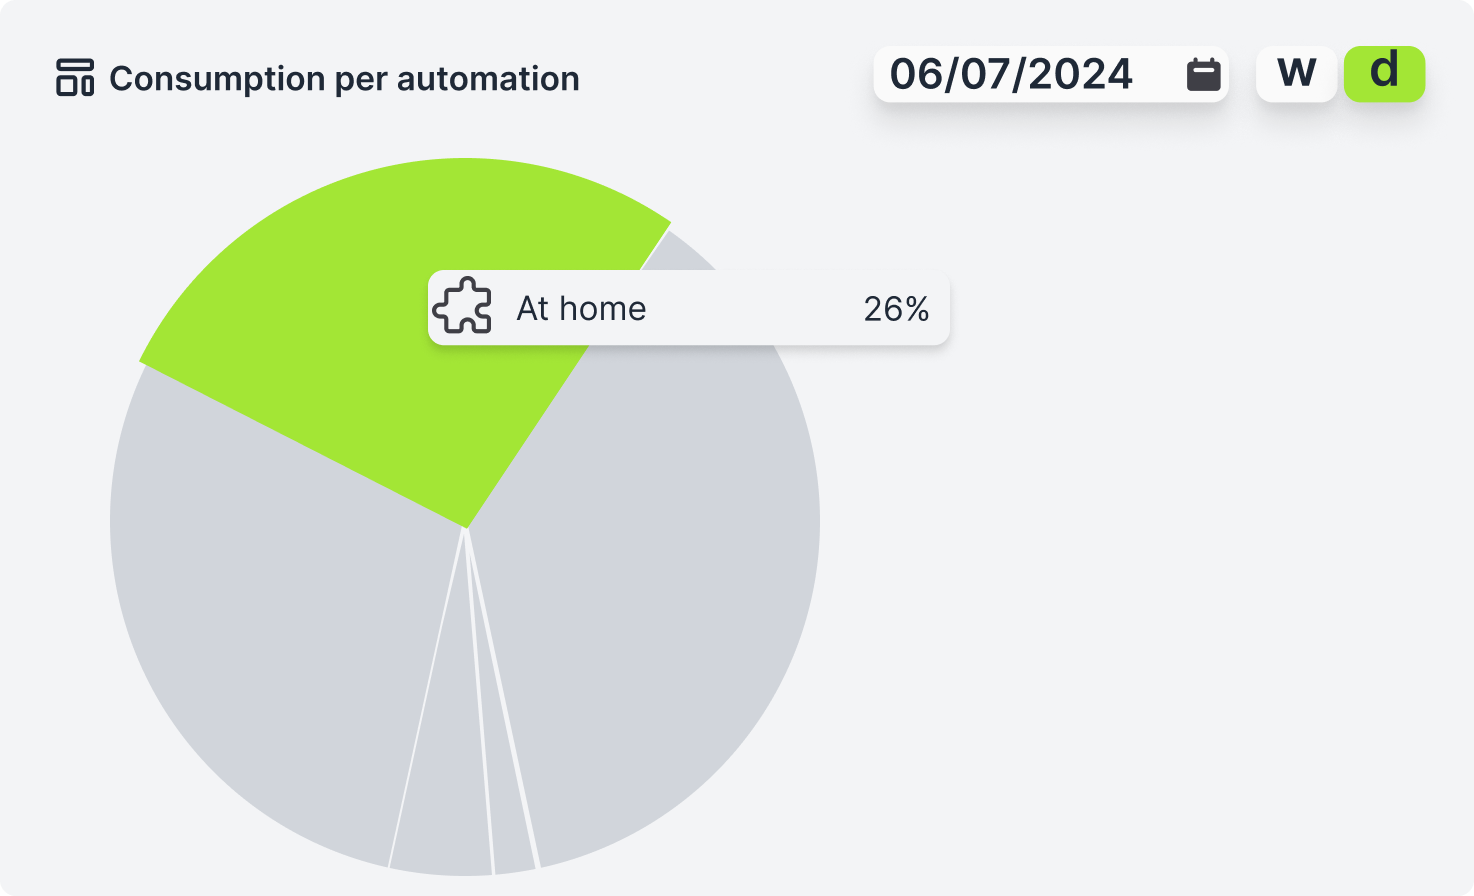
\includegraphics[width=0.95\linewidth]{images/Chap - 4/Timespan=Day, Mode=Automation energy, Graph=Pie, Date=Past.png}
    \caption{Sistema di partenza: consumo per automazione (torta)}
    \label{fig:cap4_base_automation_pie}
\end{figure}

Infine, è presente anche una vista settimanale per persona (fig.~\ref{fig:cap4_base_person_week}), utile quando nella casa sono presenti più utenti.

\begin{figure}[H]
    \centering
    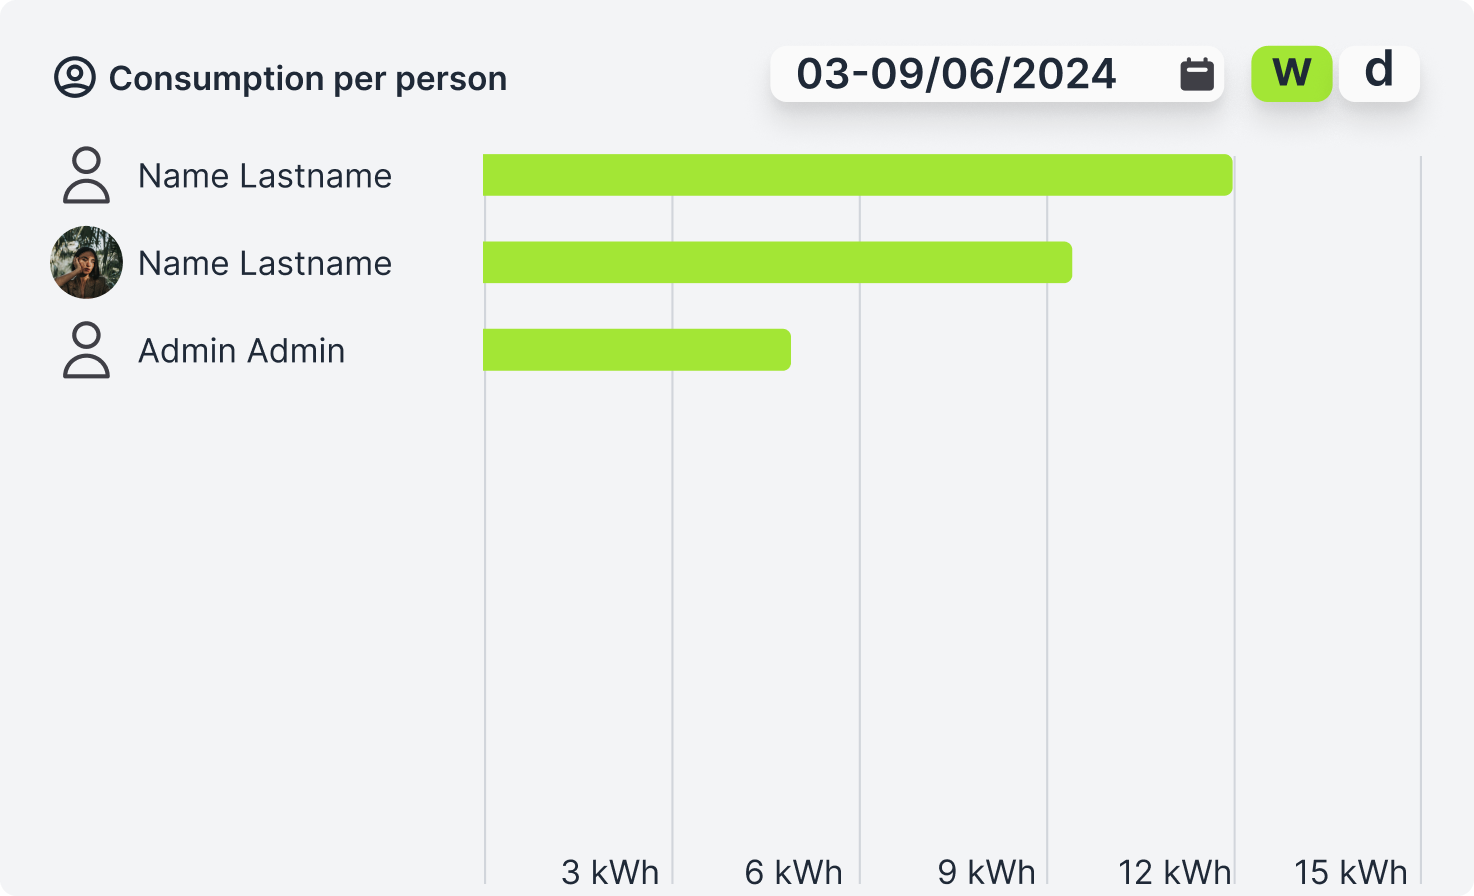
\includegraphics[width=0.95\linewidth]{images/Chap - 4/Timespan=Week, Mode=Person energy, Graph=Bar, Date=Past.png}
    \caption{Sistema di partenza: consumo energetico per persona}
    \label{fig:cap4_base_person_week}
\end{figure}

\subsection{Configurazione iniziale della casa}
Una parte importante del sistema di partenza è il \textit{wizard} di configurazione iniziale, attraverso il quale l'utente imposta planimetria, dispositivi e piano energetico.

Il primo step richiede il caricamento della planimetria (fig.~\ref{fig:cap4_base_config_step0}).

\begin{figure}[H]
    \centering
    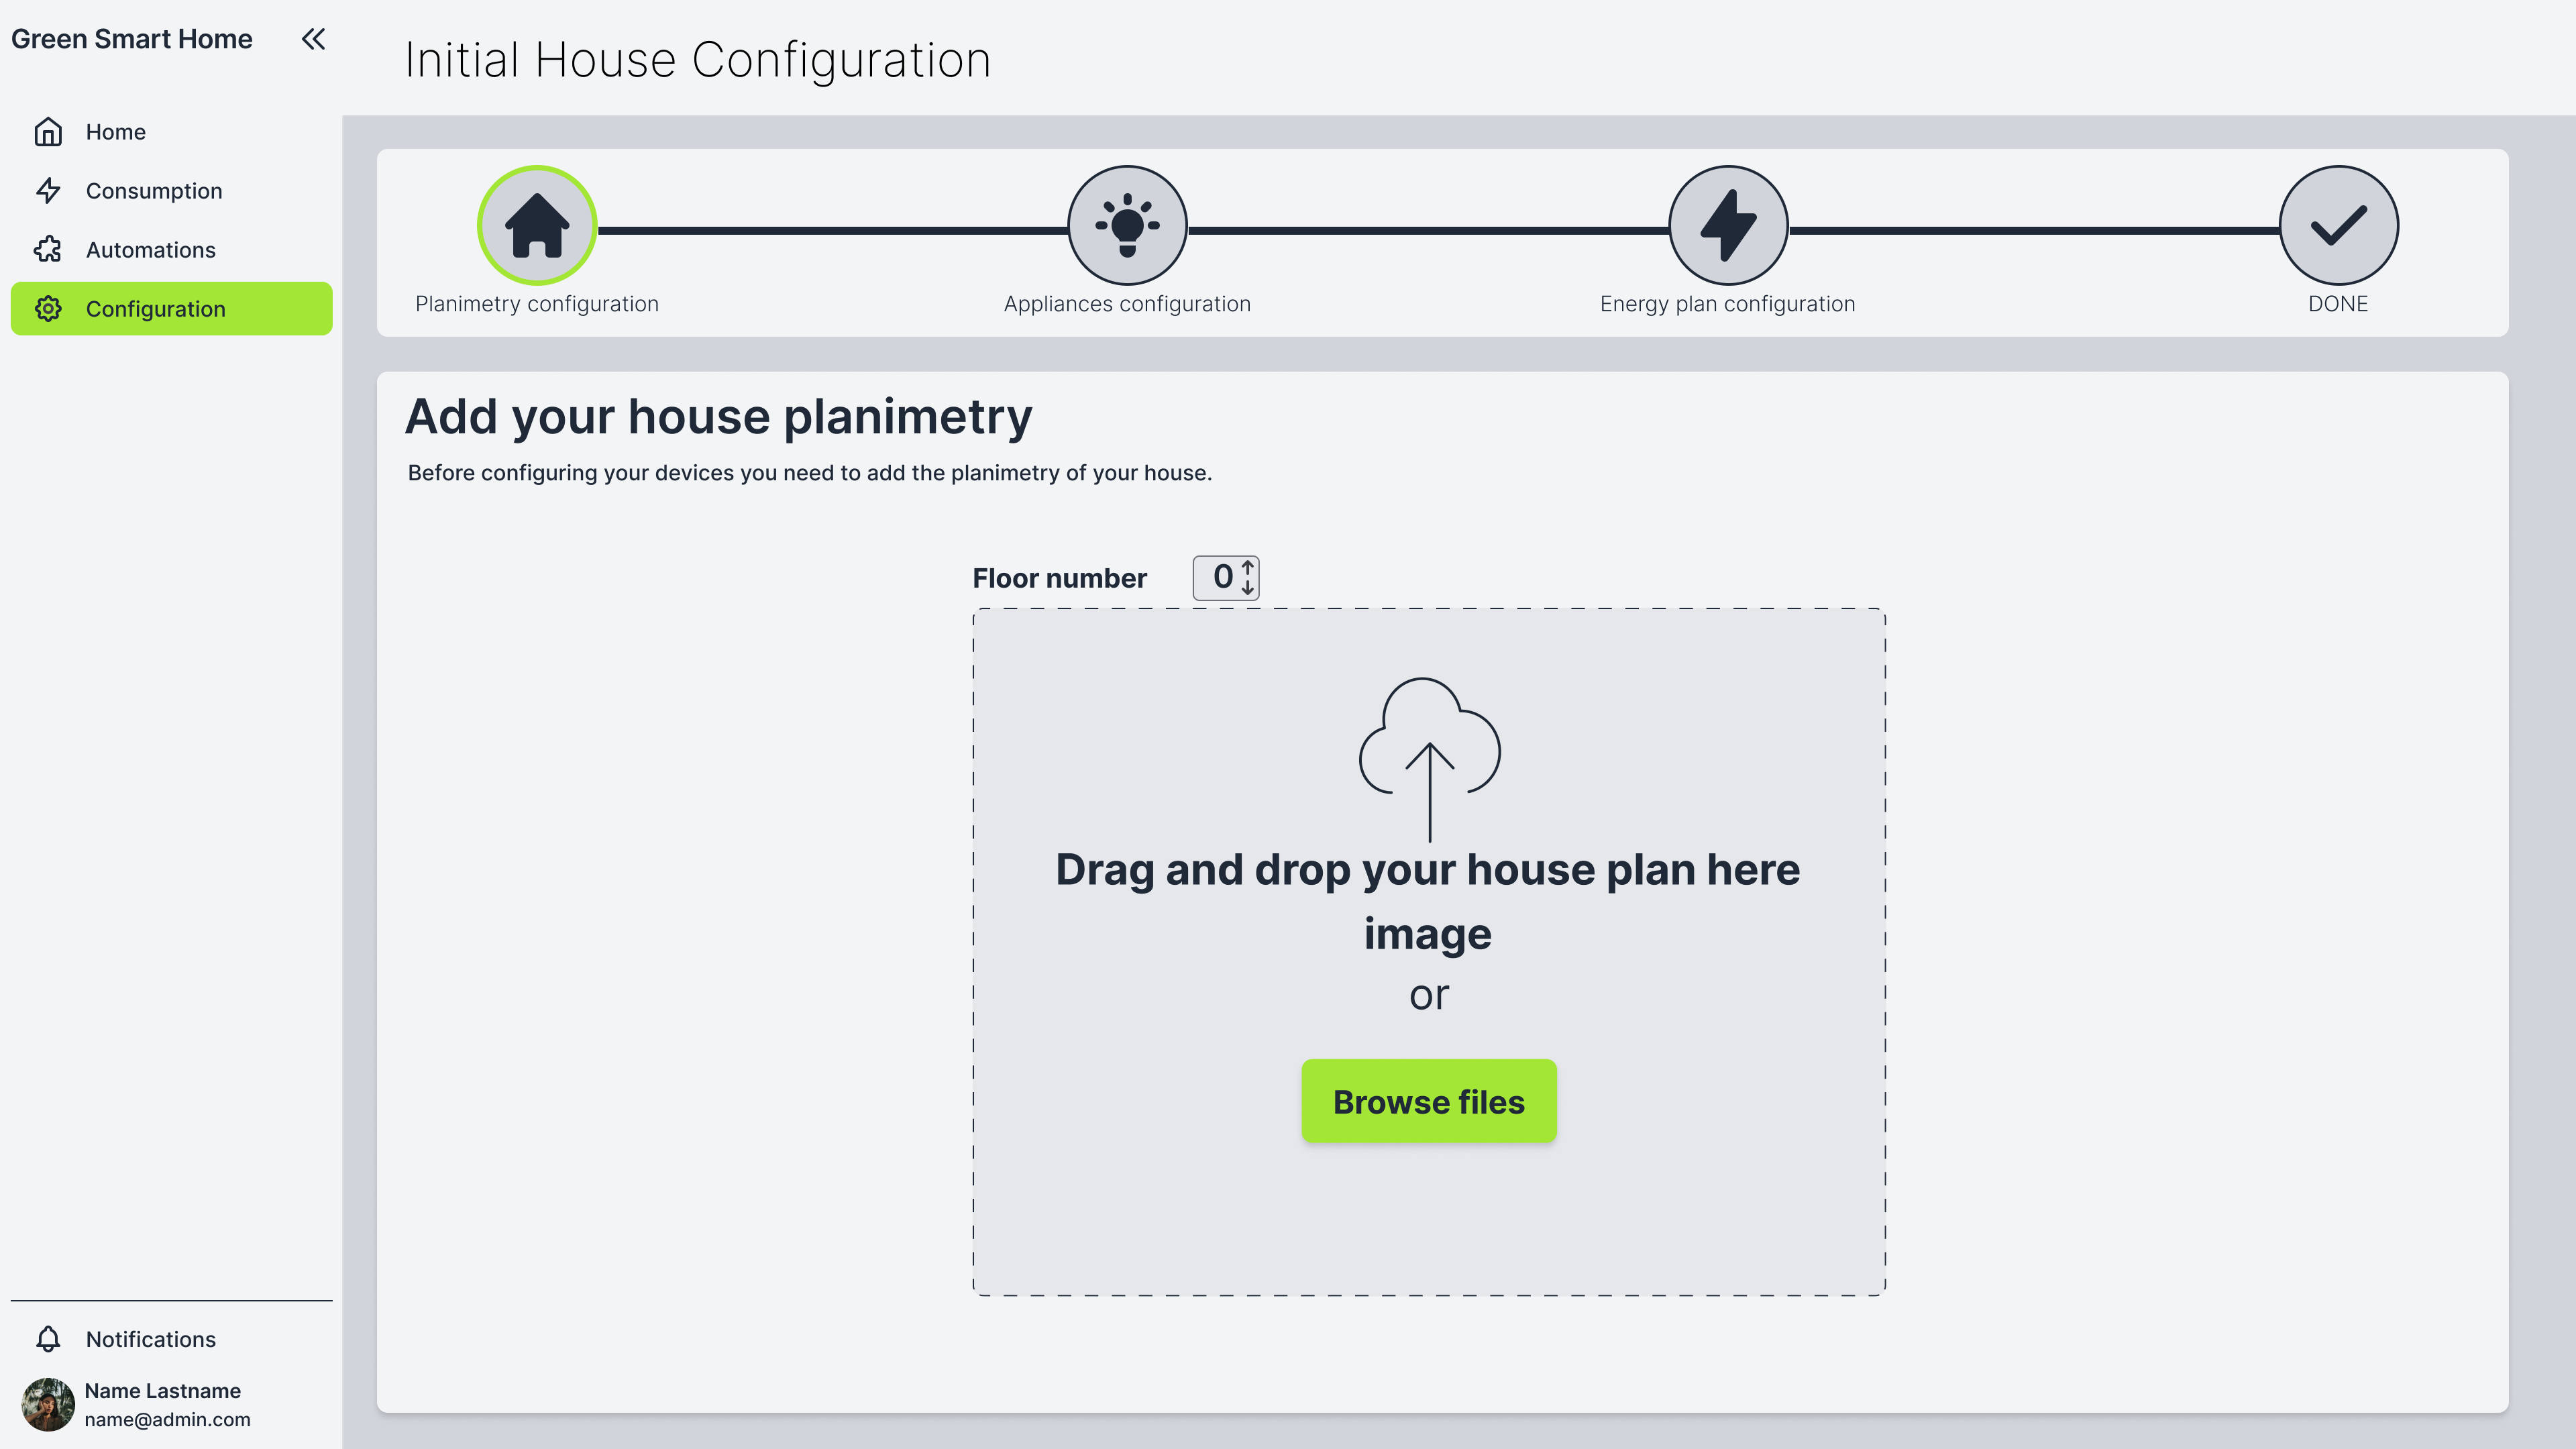
\includegraphics[width=1\linewidth]{images/Chap - 4/House configration_0.png}
    \caption{Sistema di partenza: step iniziale con caricamento planimetria}
    \label{fig:cap4_base_config_step0}
\end{figure}

Una volta caricata la mappa, è possibile aggiungere/rimuovere piani e salvare la configurazione del piano corrente (fig.~\ref{fig:cap4_base_config_step2}).

\begin{figure}[H]
    \centering
    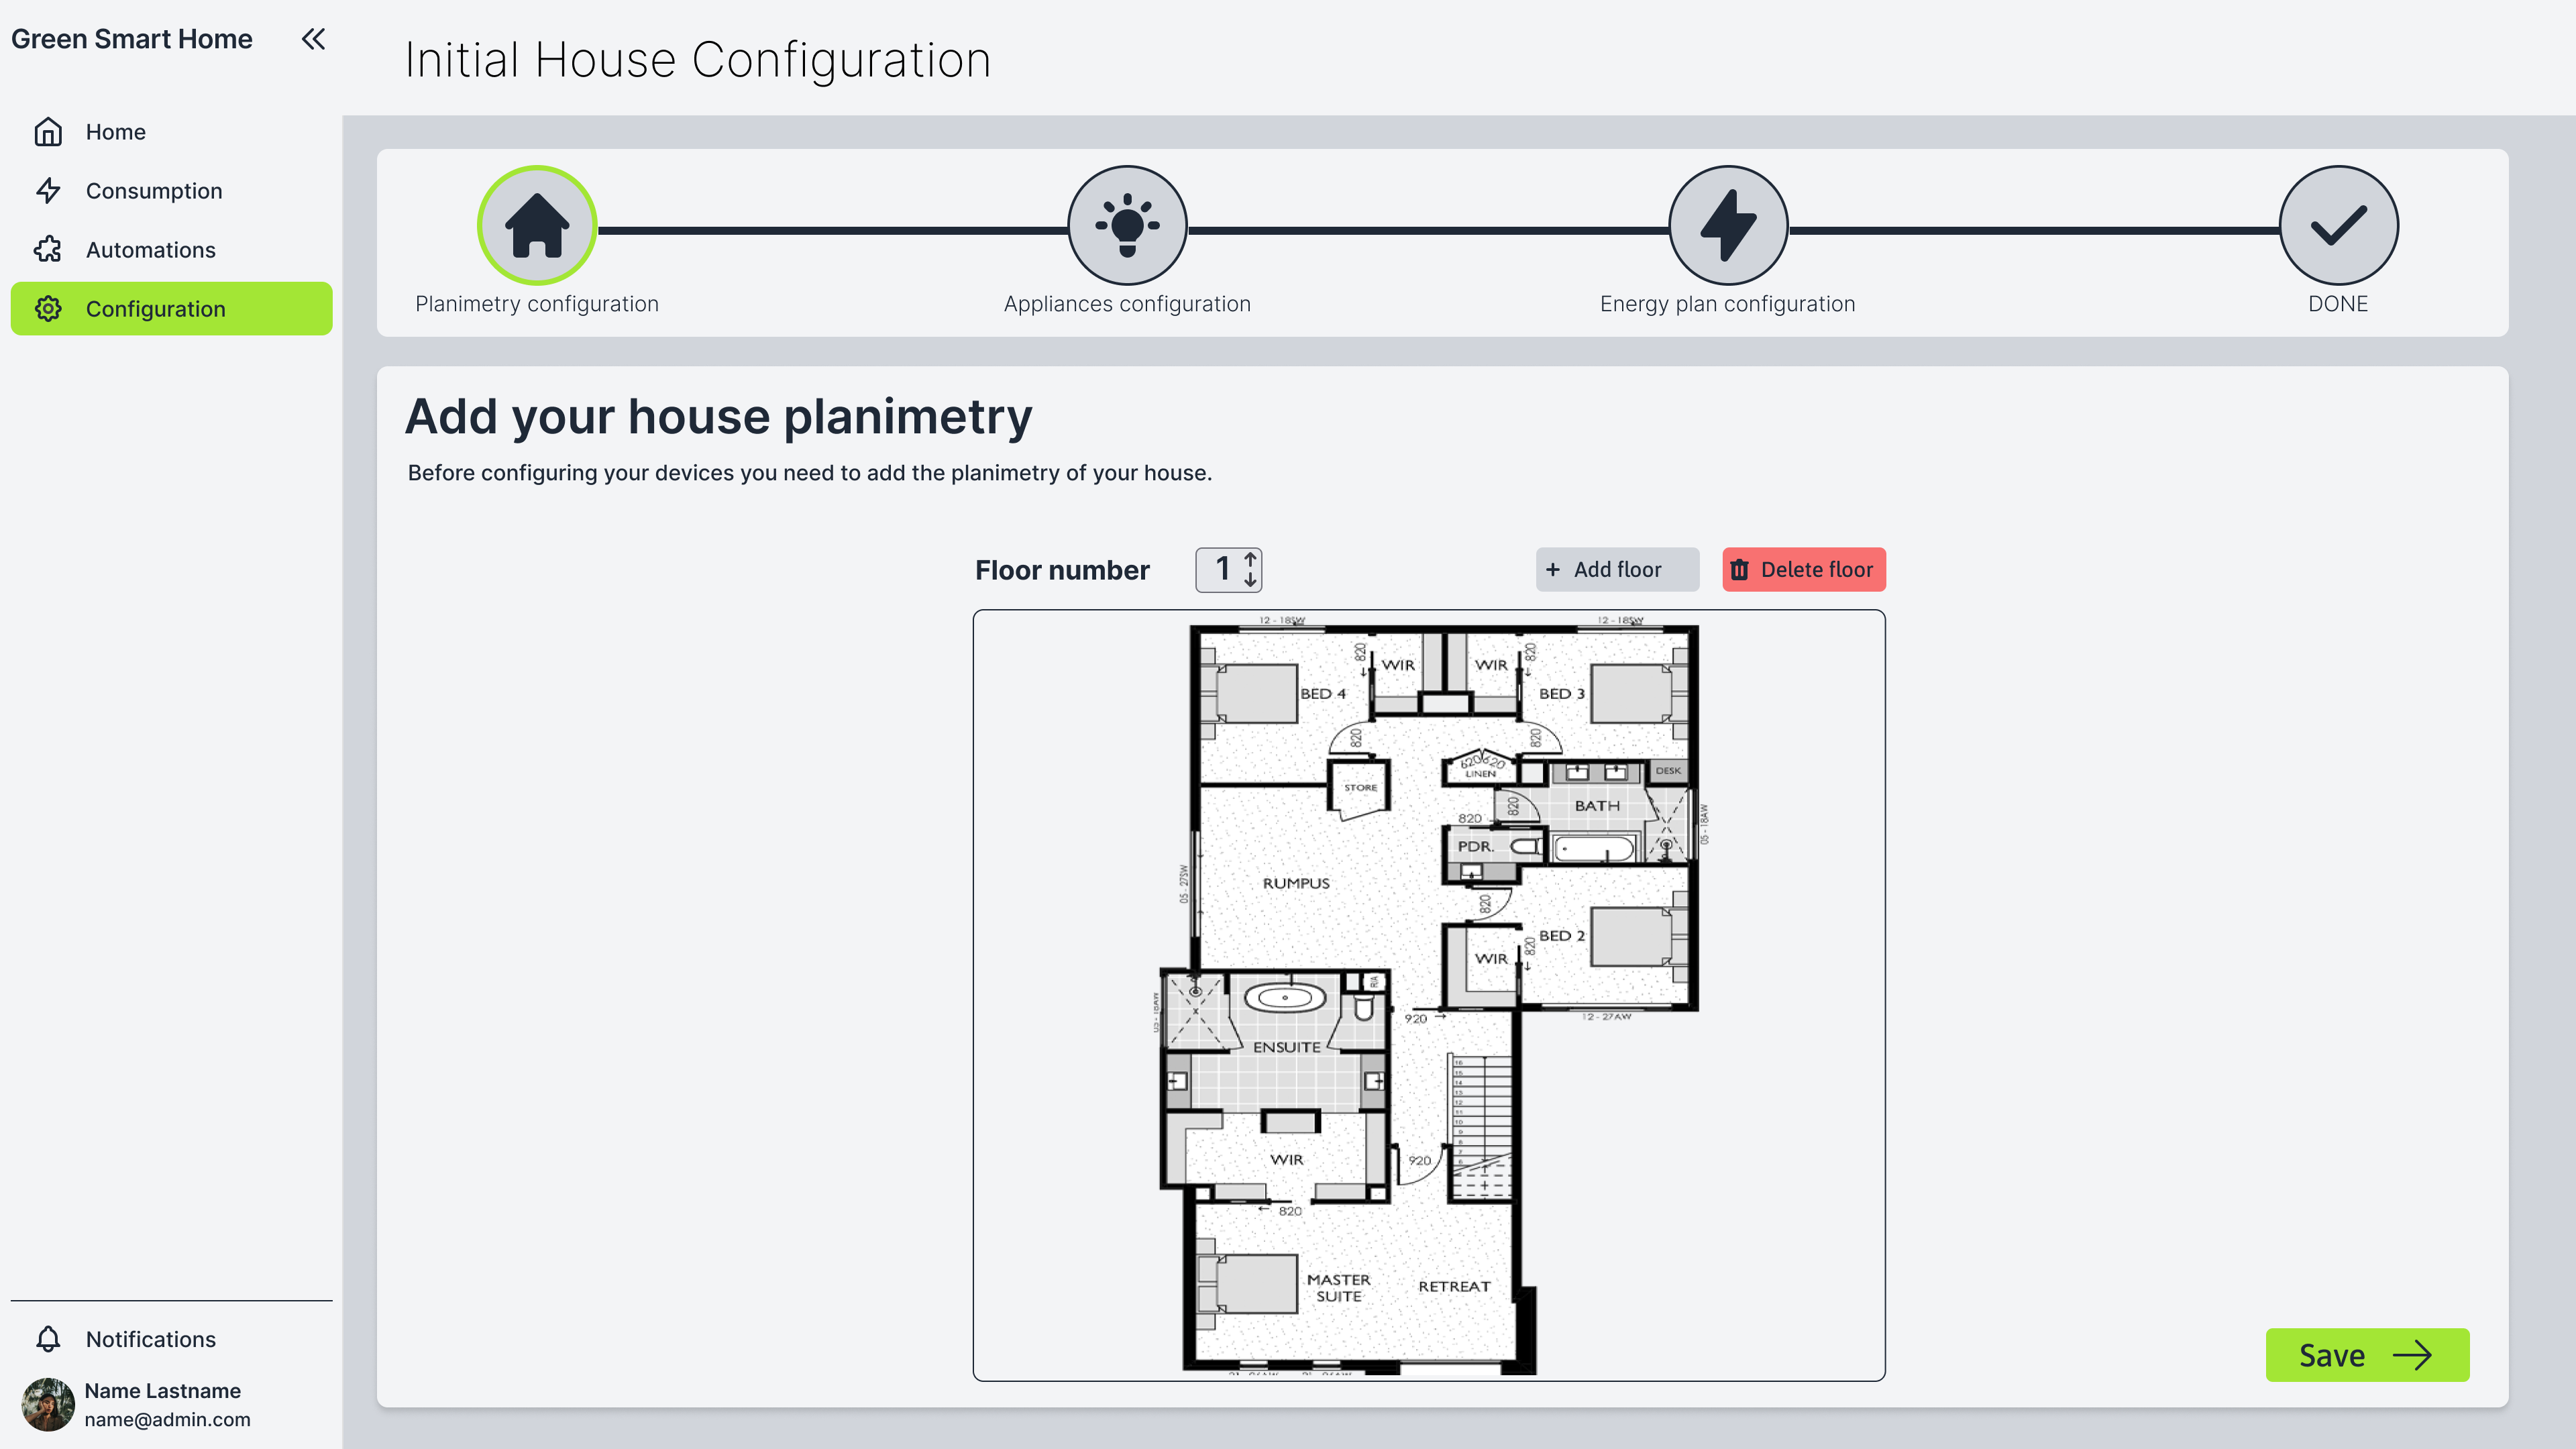
\includegraphics[width=1\linewidth]{images/Chap - 4/House configration_2.png}
    \caption{Sistema di partenza: planimetria caricata e gestione dei piani}
    \label{fig:cap4_base_config_step2}
\end{figure}

Successivamente si passa allo step dedicato al posizionamento dei dispositivi sulla mappa della casa, con drag-and-drop delle appliance (fig.~\ref{fig:cap4_base_config_step4}).

\begin{figure}[H]
    \centering
    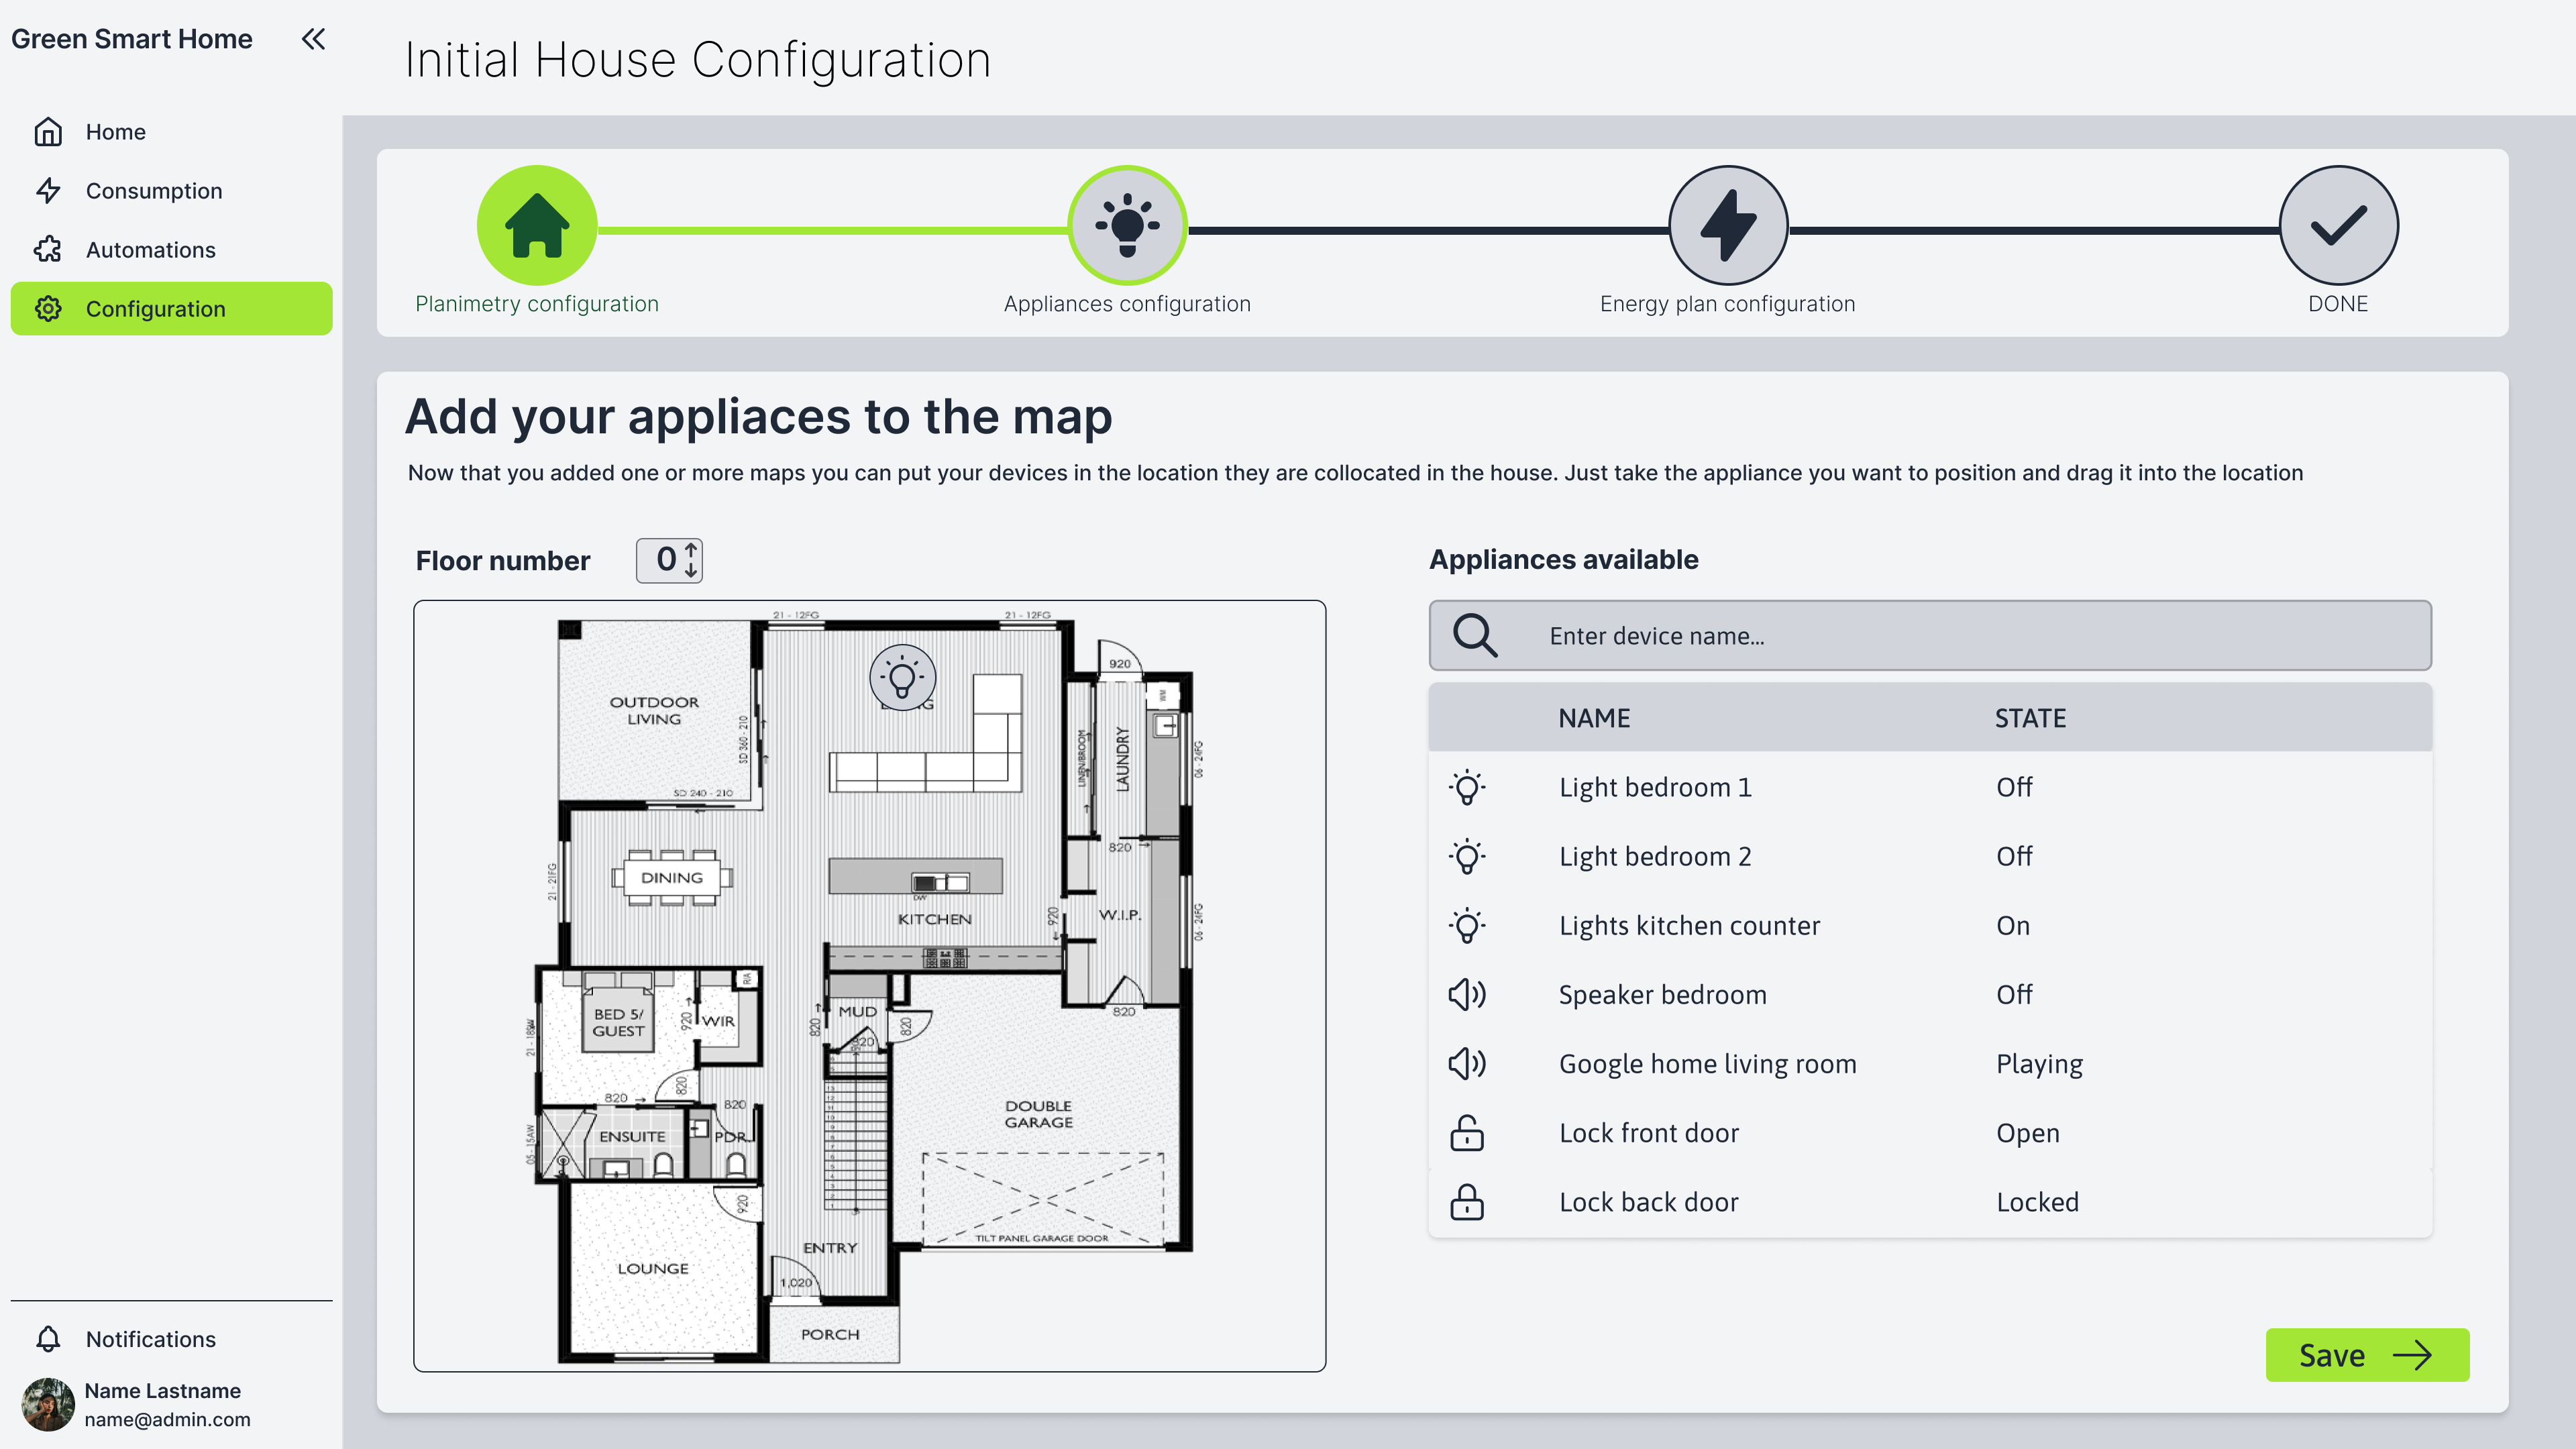
\includegraphics[width=1\linewidth]{images/Chap - 4/House configration_4.png}
    \caption{Sistema di partenza: configurazione e posizionamento delle appliance}
    \label{fig:cap4_base_config_step4}
\end{figure}

Il terzo step riguarda il piano energetico, con numero di fasce, costo per fascia e potenza massima disponibile (fig.~\ref{fig:cap4_base_config_step7}).

\begin{figure}[H]
    \centering
    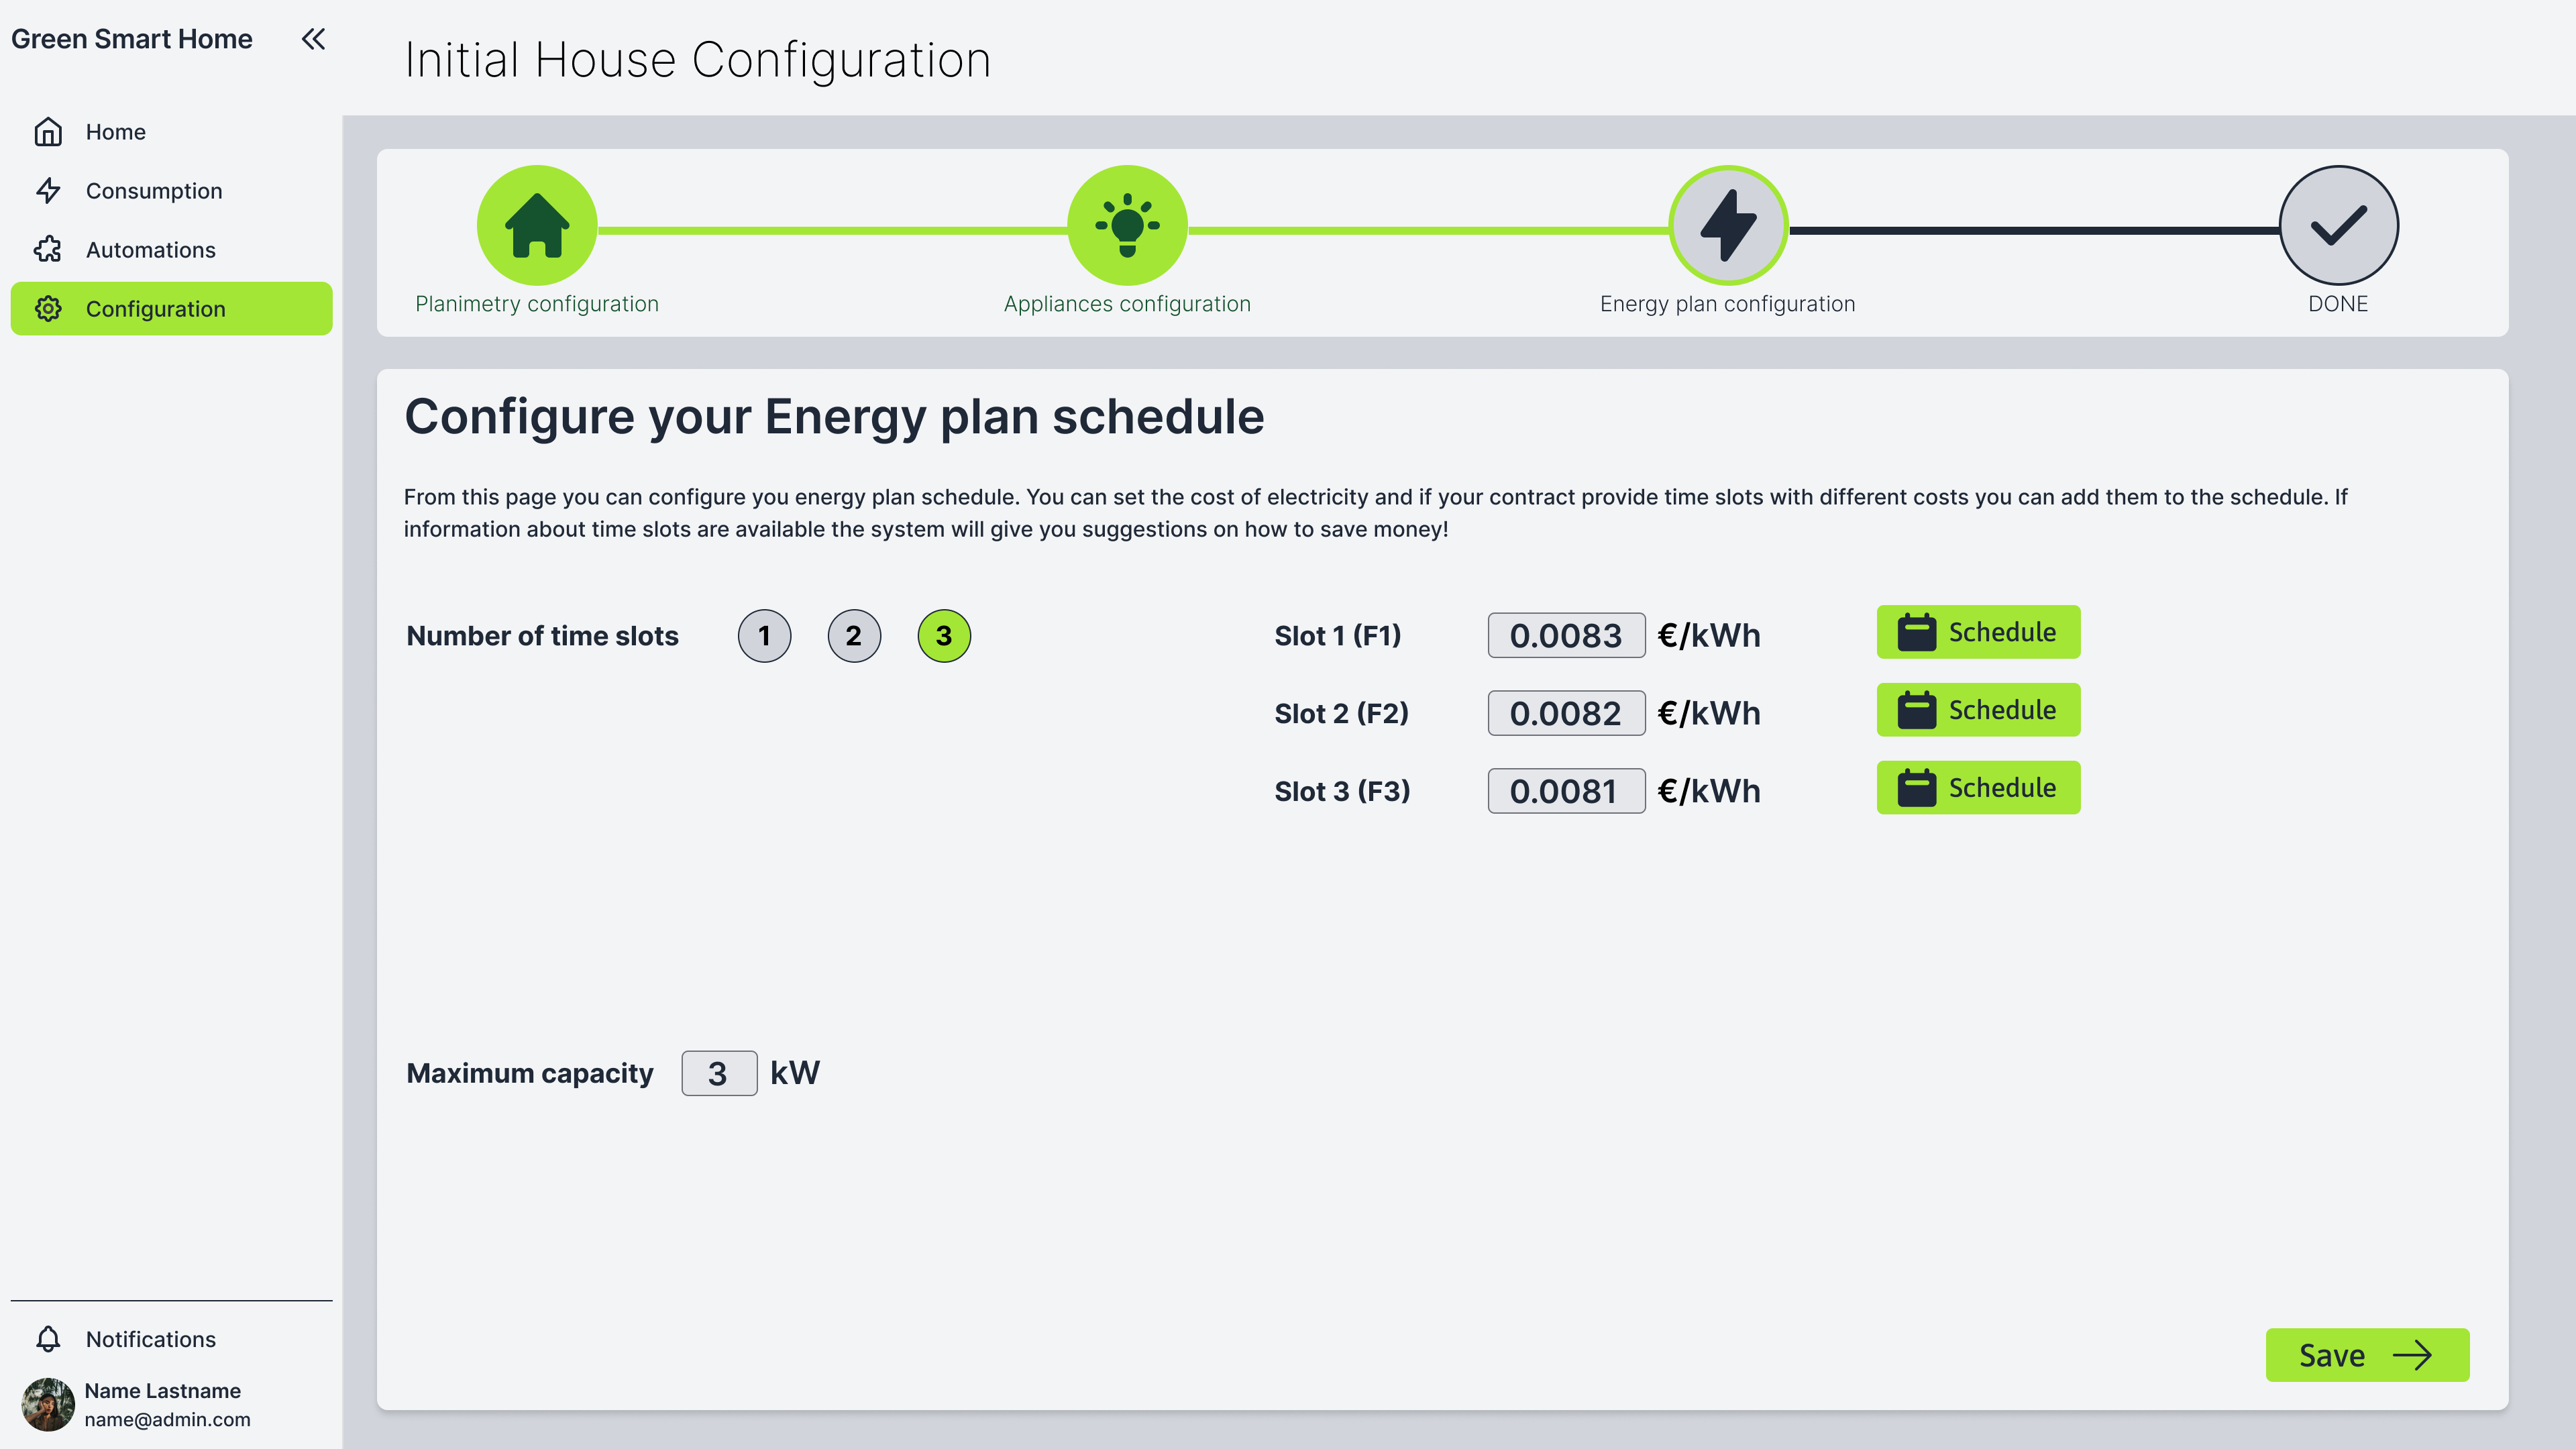
\includegraphics[width=1\linewidth]{images/Chap - 4/House configration_7.png}
    \caption{Sistema di partenza: configurazione del piano energetico iniziale}
    \label{fig:cap4_base_config_step7}
\end{figure}

Al termine del processo viene mostrata una conferma di configurazione completata (fig.~\ref{fig:cap4_base_config_done}).

\begin{figure}[H]
    \centering
    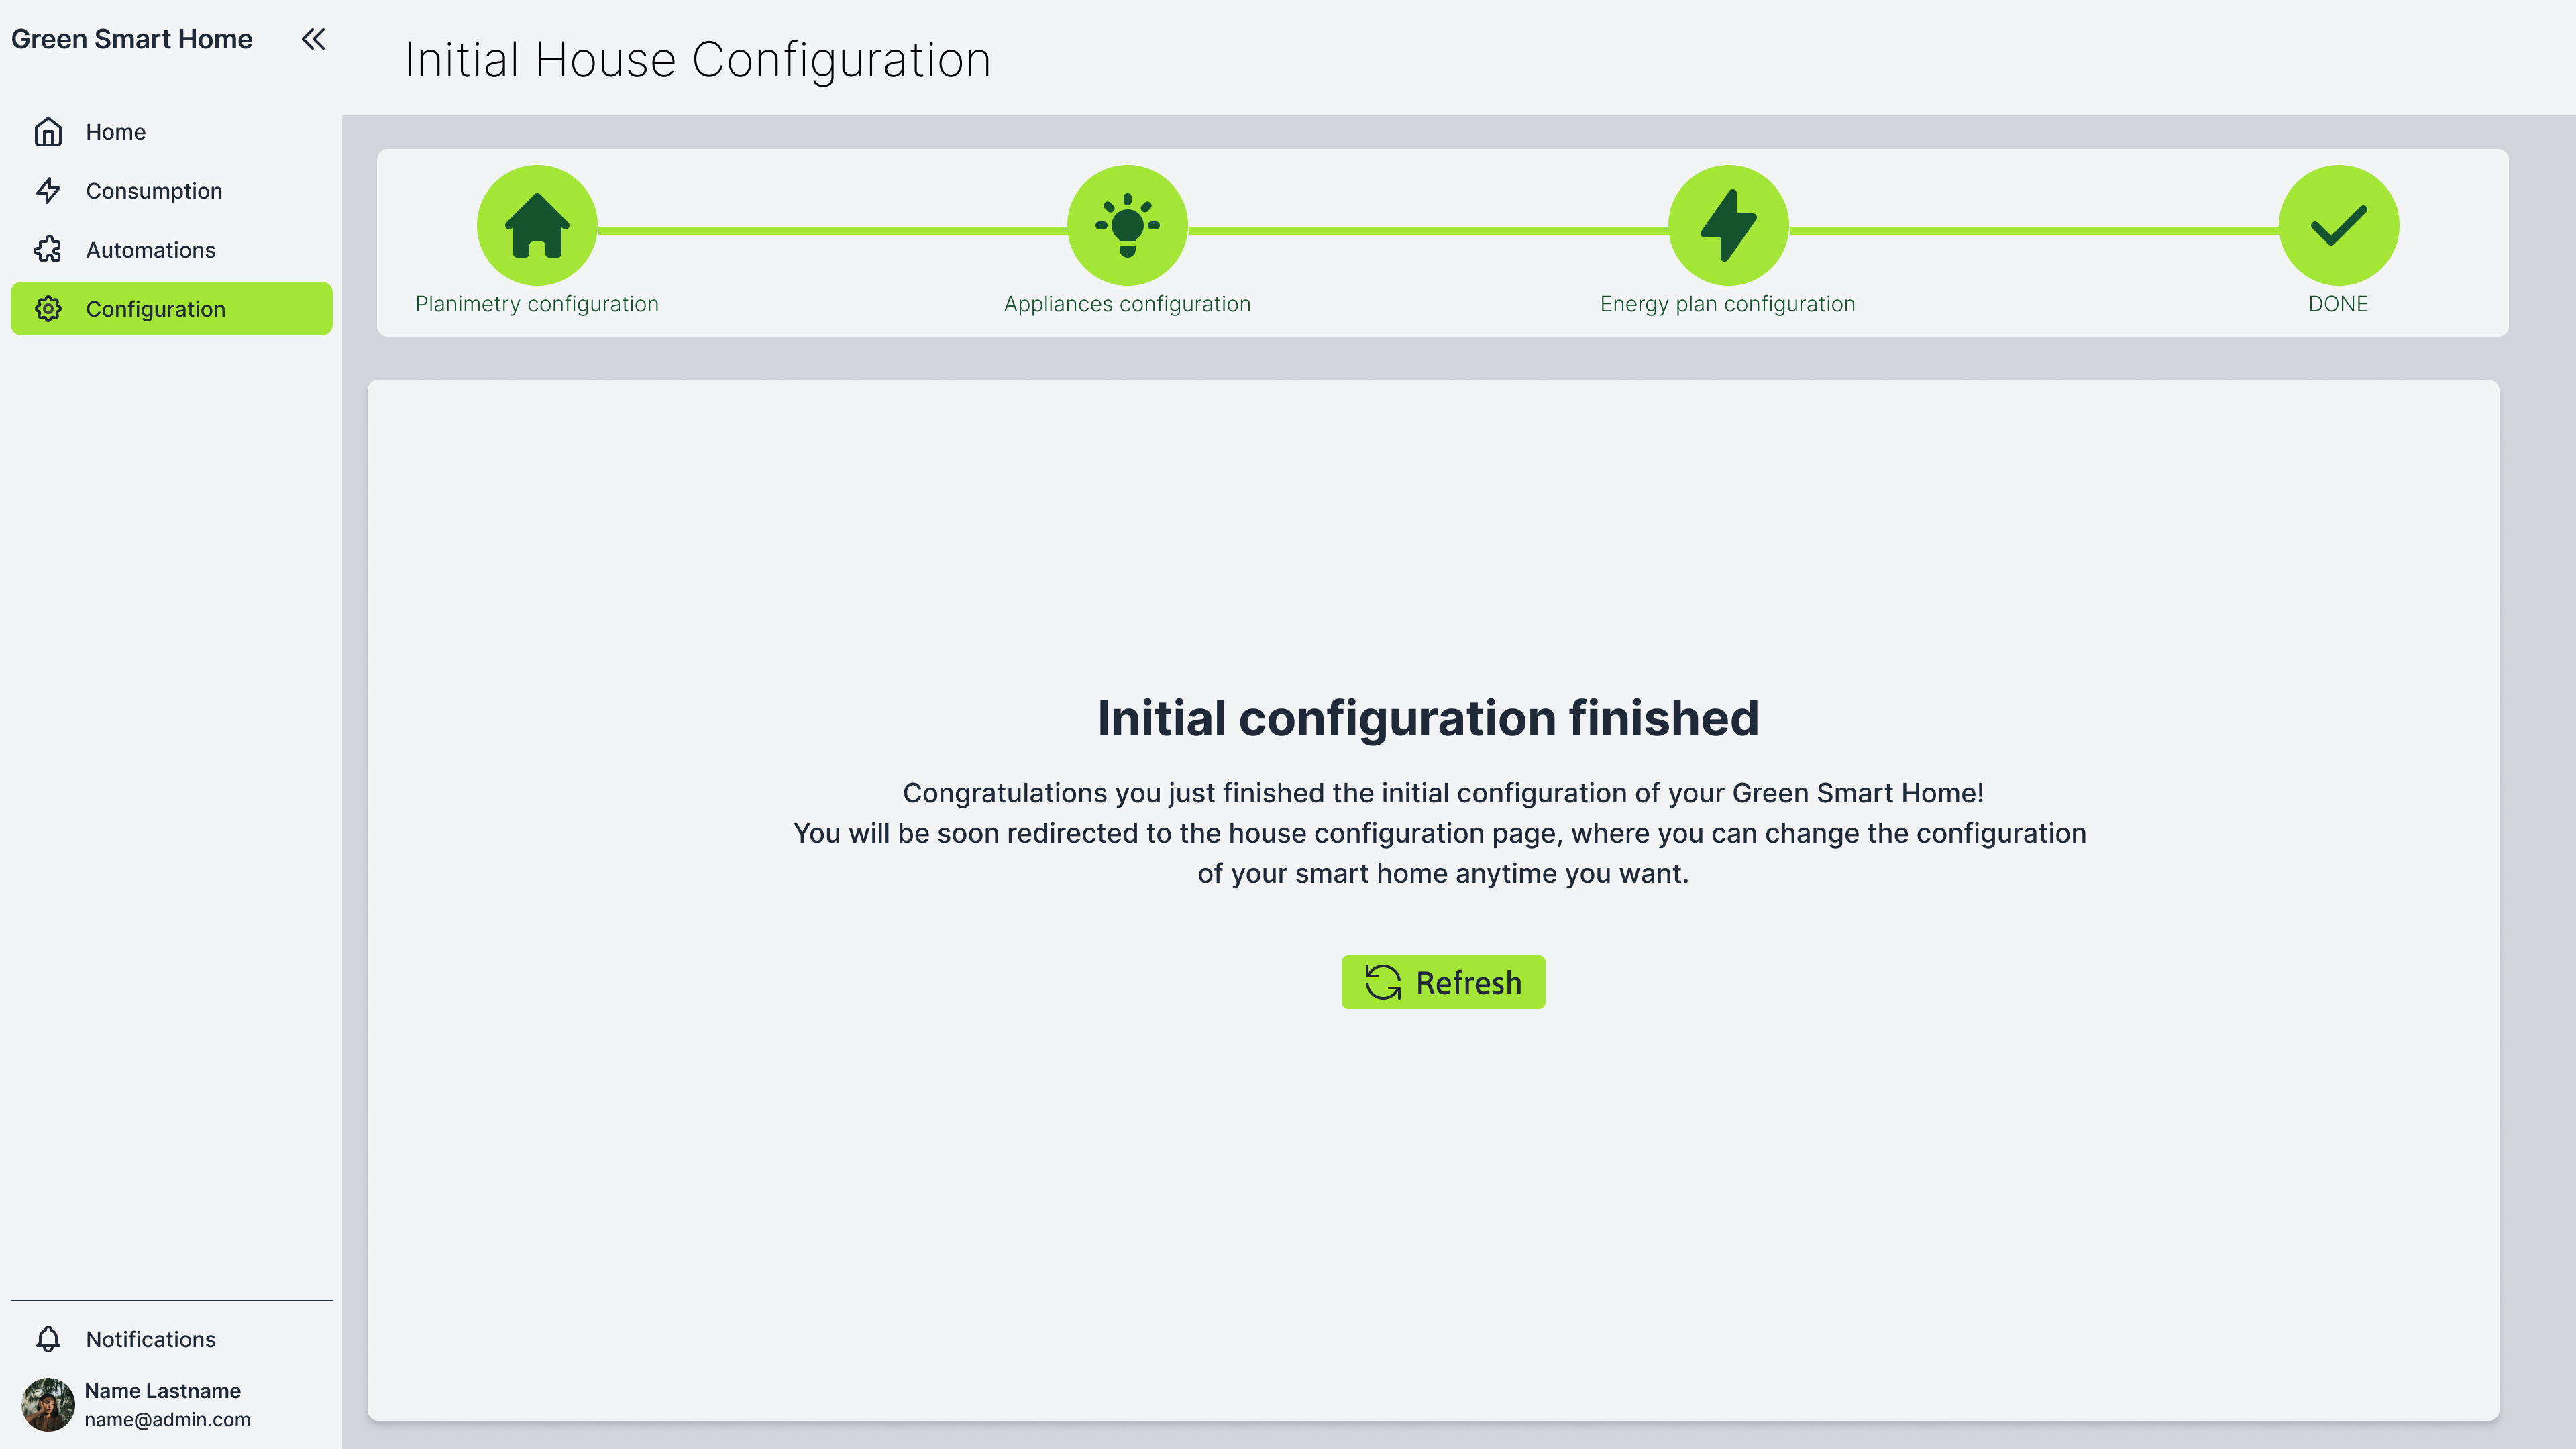
\includegraphics[width=1\linewidth]{images/Chap - 4/House configration_8.png}
    \caption{Sistema di partenza: conferma completamento configurazione iniziale}
    \label{fig:cap4_base_config_done}
\end{figure}

Dopo la fase iniziale, l'utente può tornare nella configurazione ordinaria della casa e modificare in qualsiasi momento appliance e piano energetico (fig.~\ref{fig:cap4_base_config_final1} e fig.~\ref{fig:cap4_base_config_final2}).

\begin{figure}[H]
    \centering
    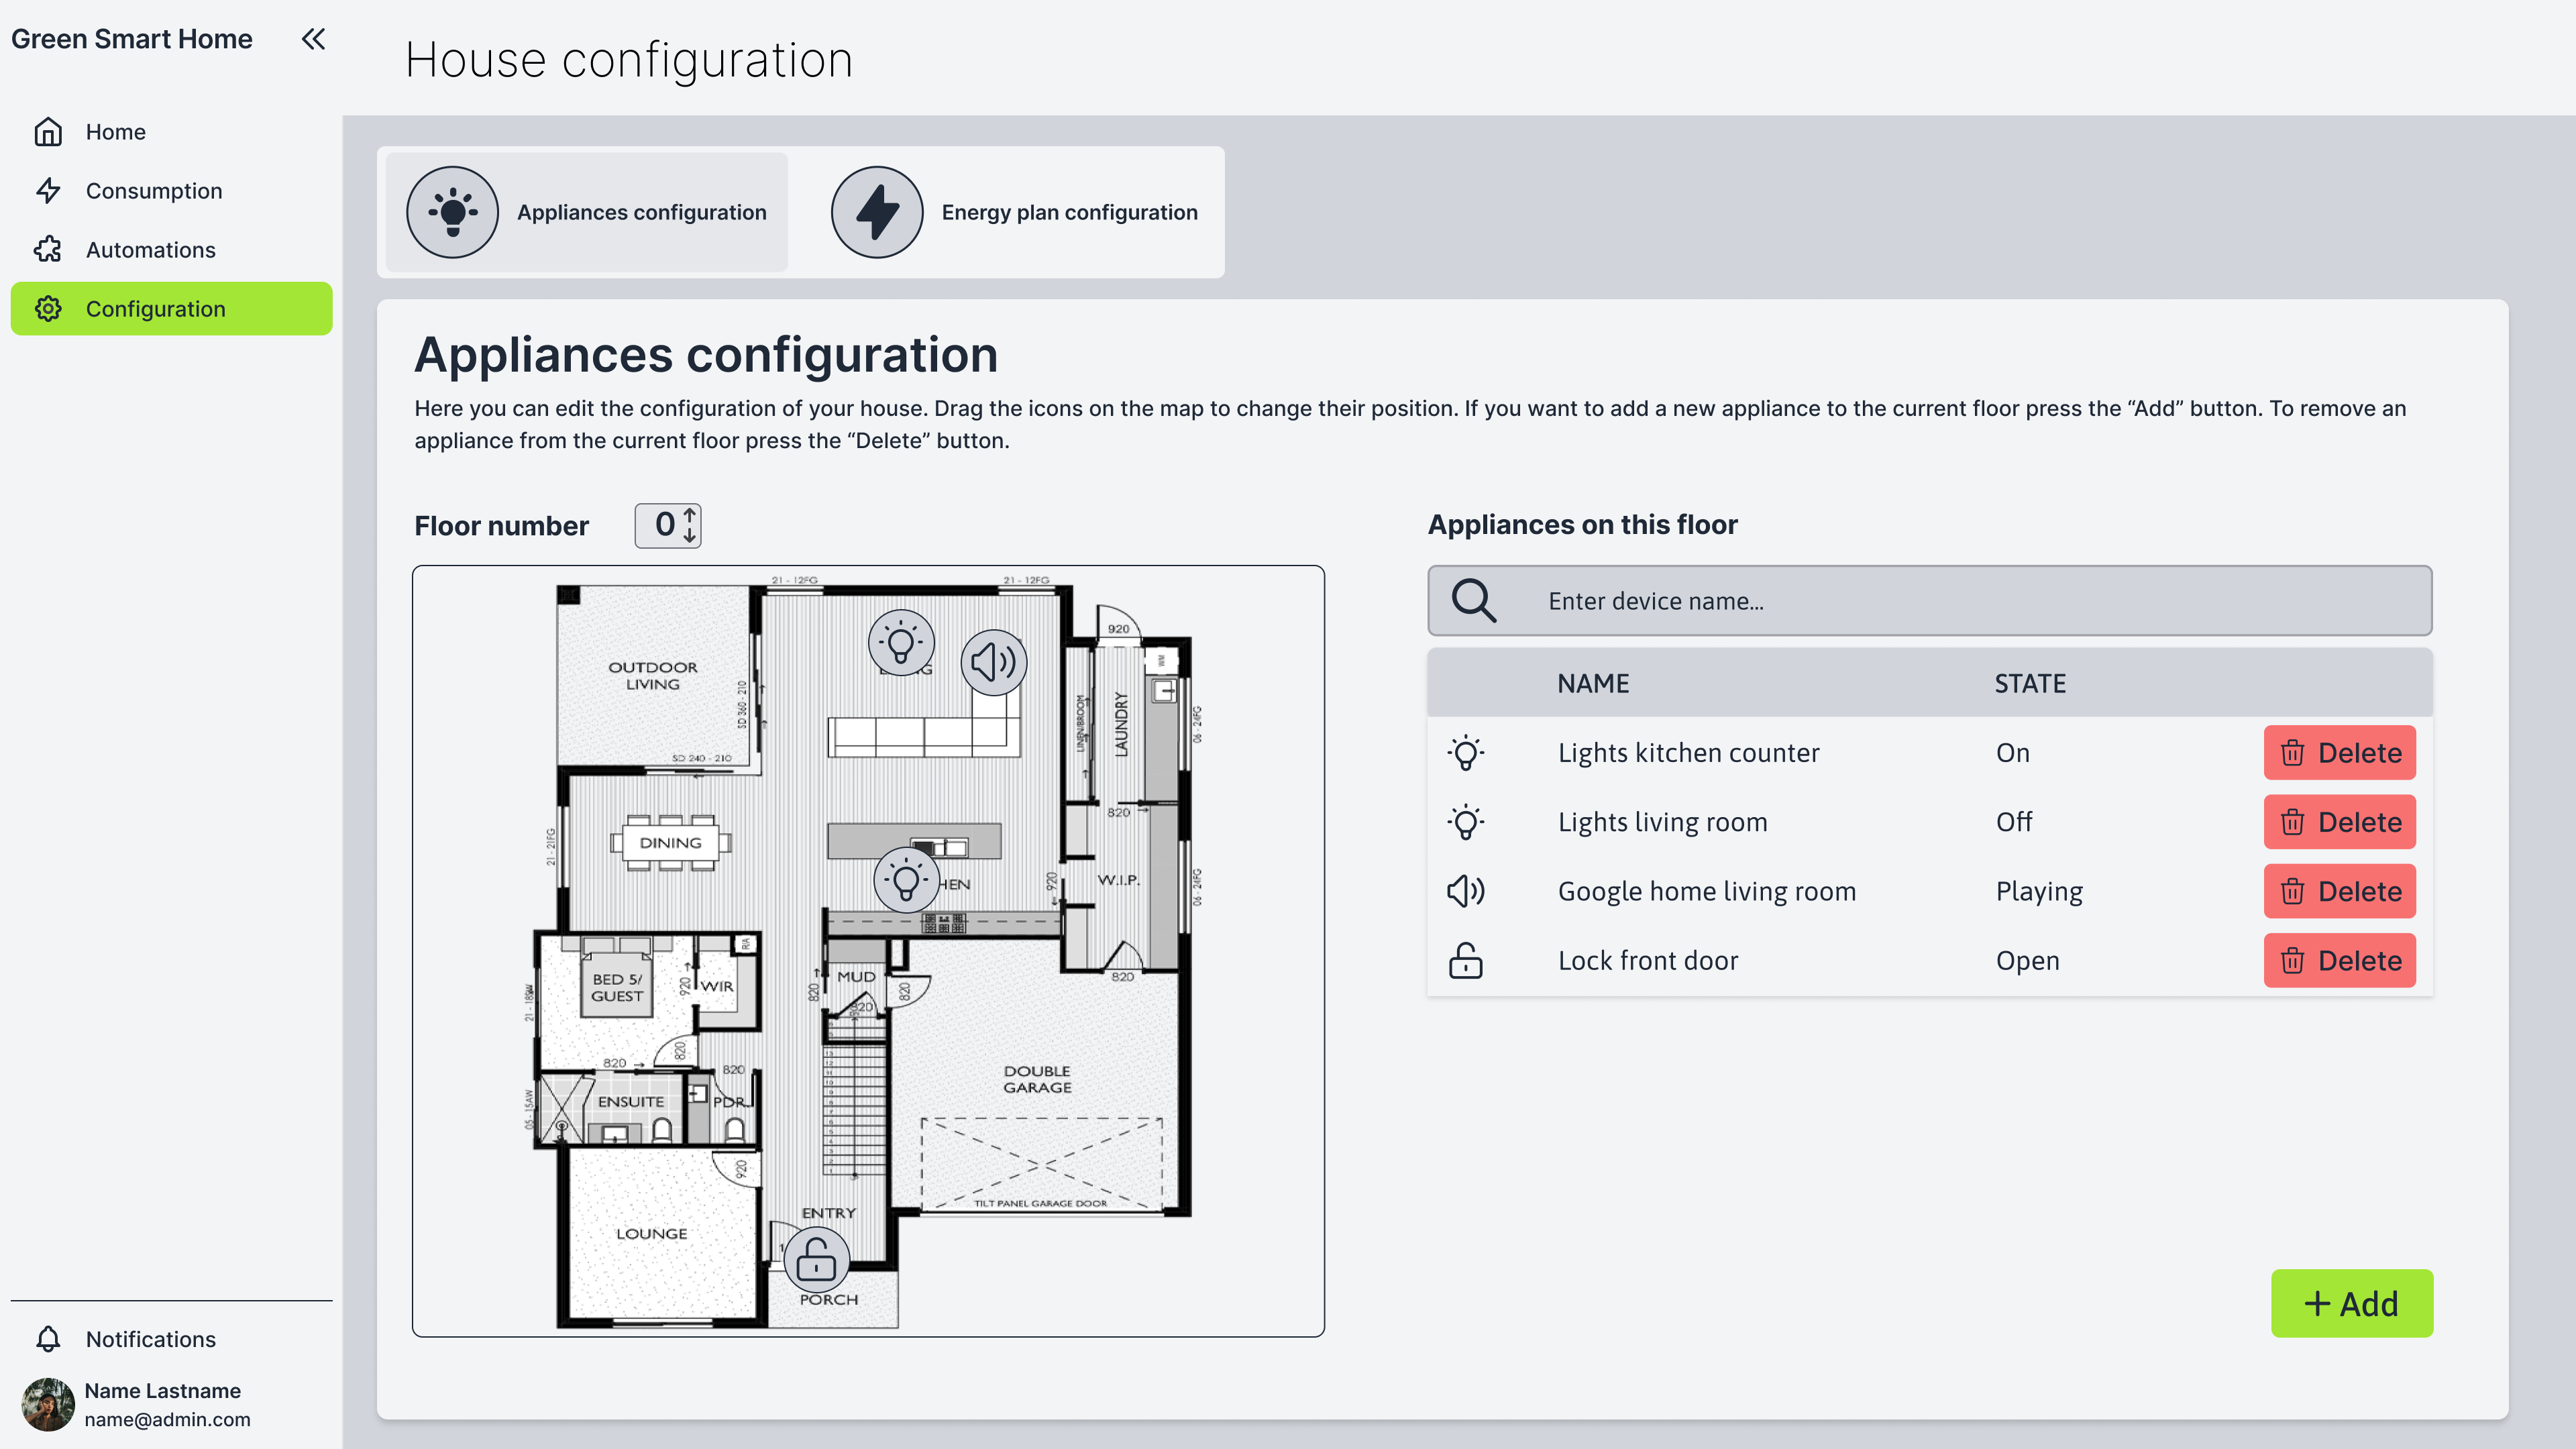
\includegraphics[width=1\linewidth]{images/Chap - 4/House configration_final_1.png}
    \caption{Sistema di partenza: pagina di configurazione appliance}
    \label{fig:cap4_base_config_final1}
\end{figure}

\begin{figure}[H]
    \centering
    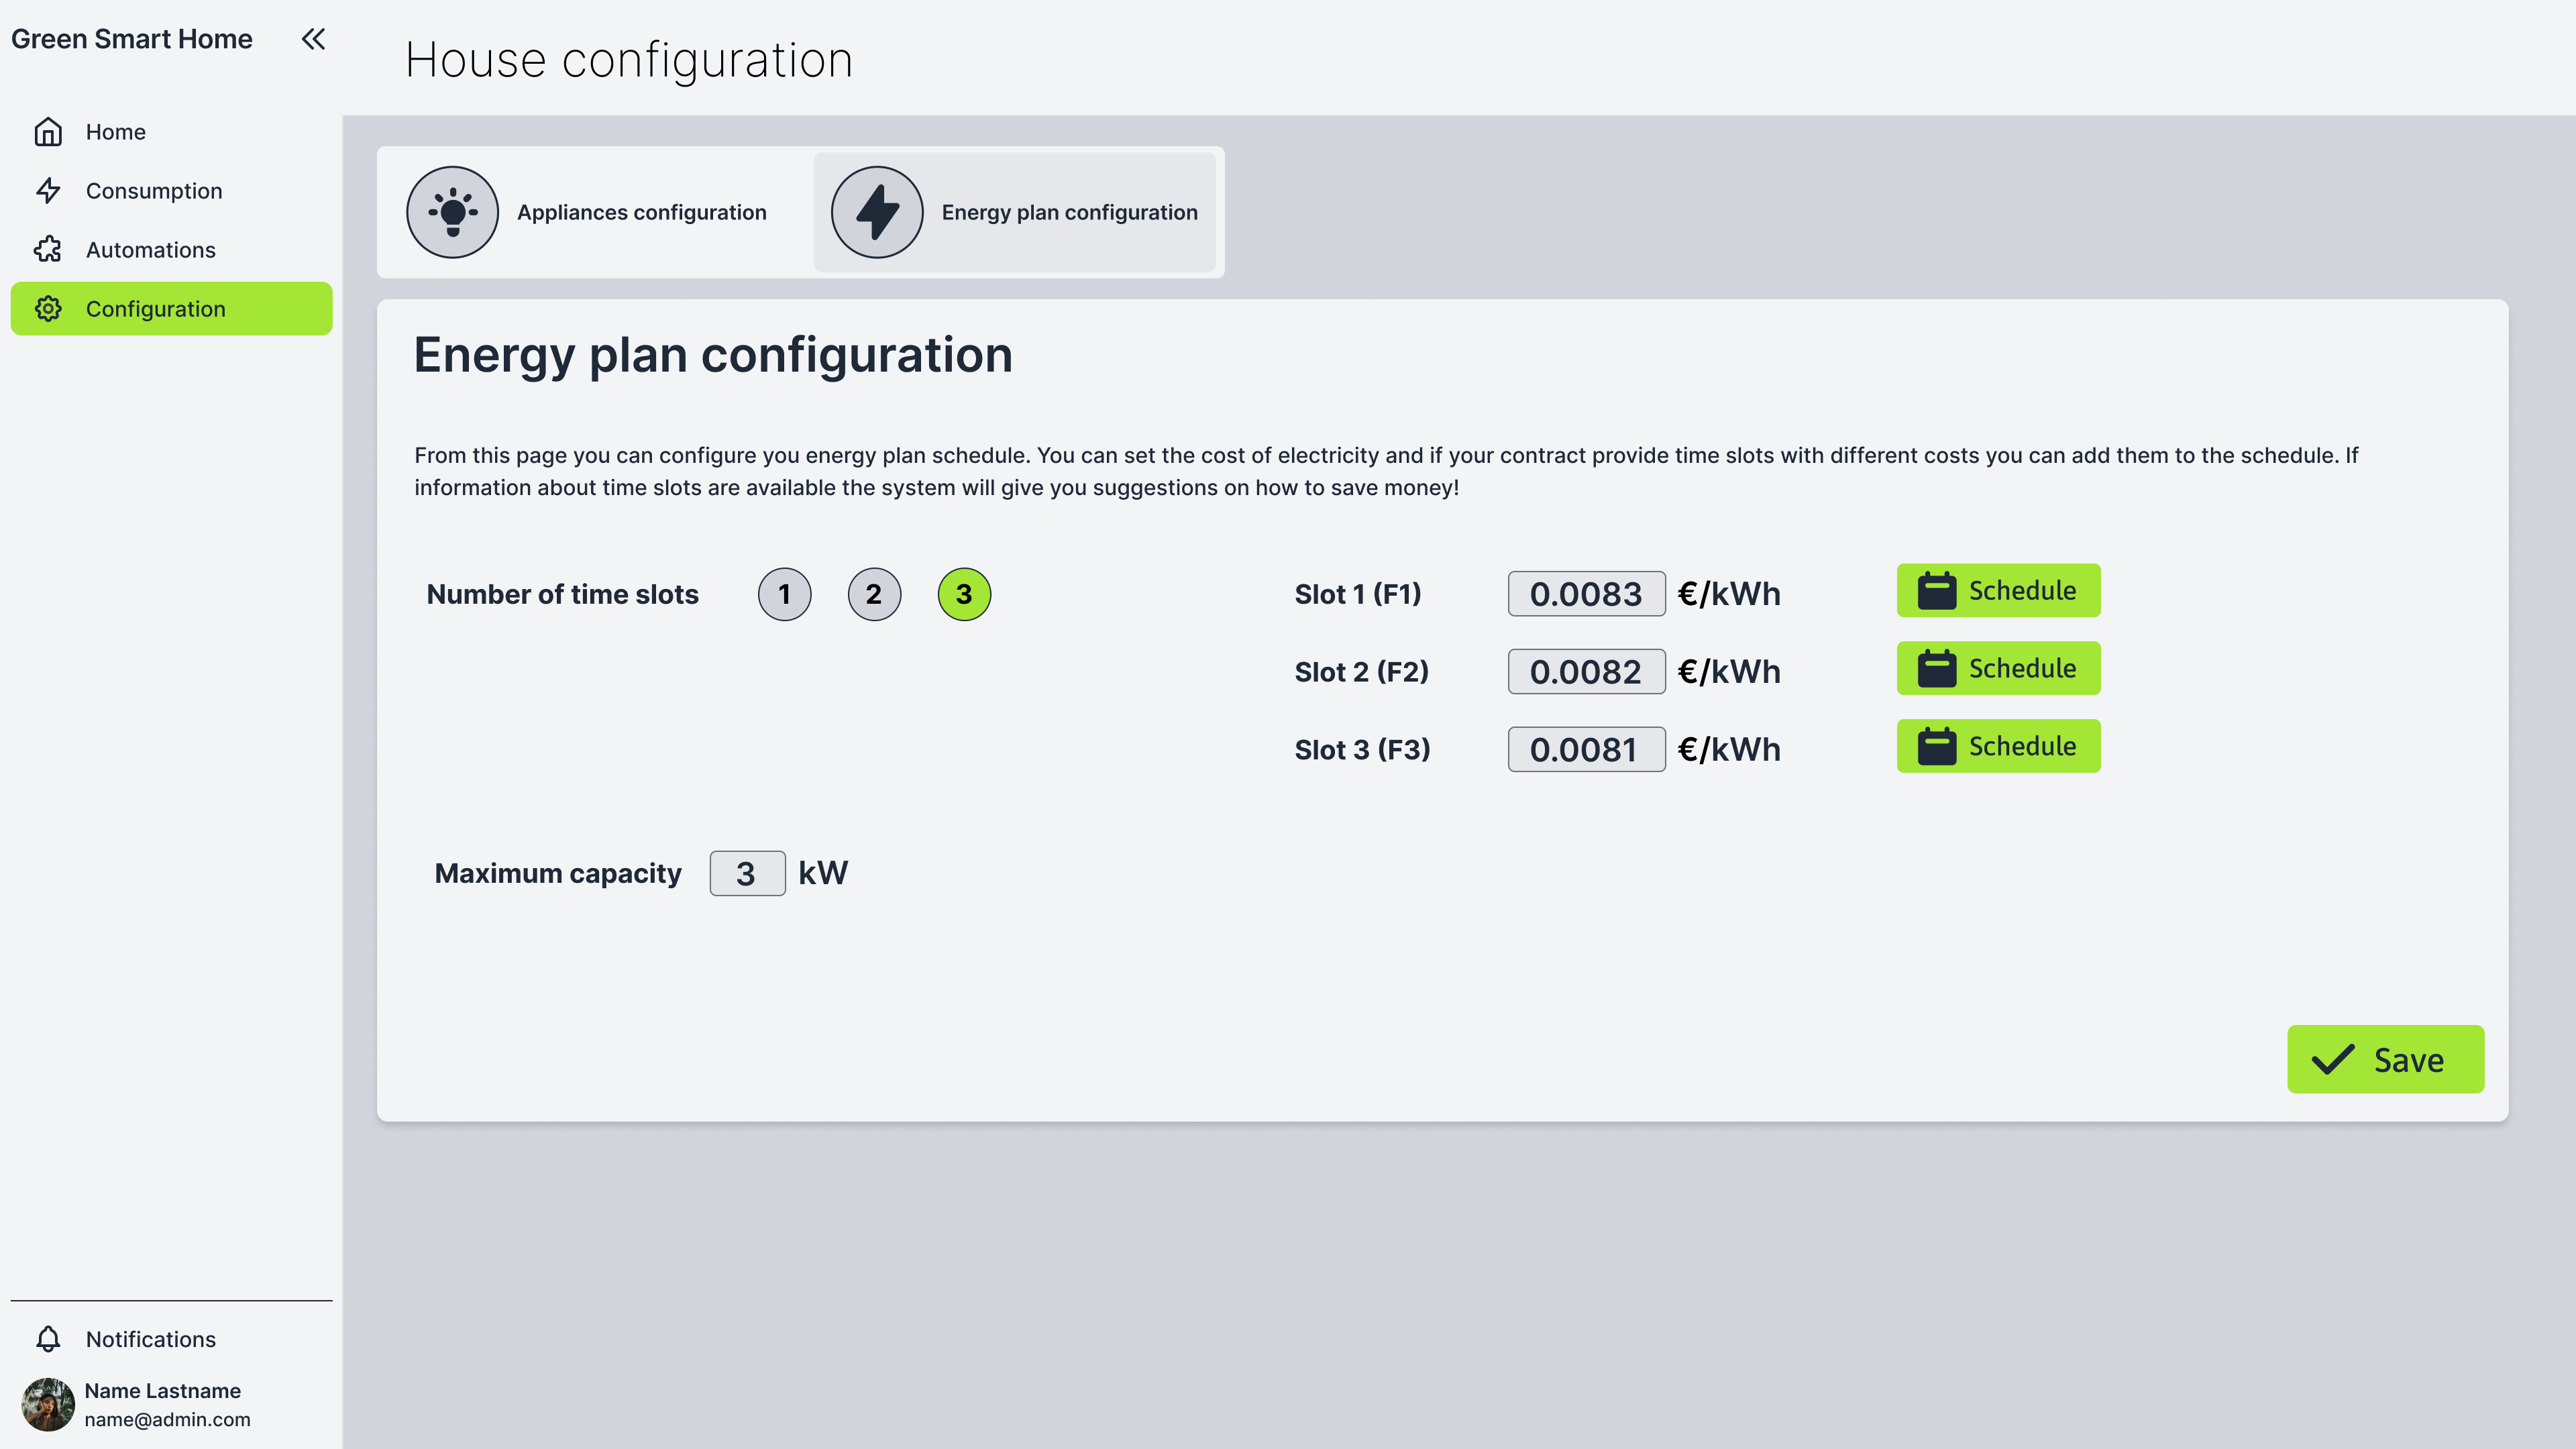
\includegraphics[width=1\linewidth]{images/Chap - 4/House configration_final_2.png}
    \caption{Sistema di partenza: pagina di configurazione piano energetico}
    \label{fig:cap4_base_config_final2}
\end{figure}

\subsection{Profilo utente, sostenibilità e componenti di supporto}
Nel sistema di partenza l'area profilo integra più funzionalità: dati anagrafici, preferenze personali, consensi privacy e sintesi dell'impronta ecologica. Una vista completa è riportata in (fig.~\ref{fig:cap4_base_profile}).

\begin{figure}[H]
    \centering
    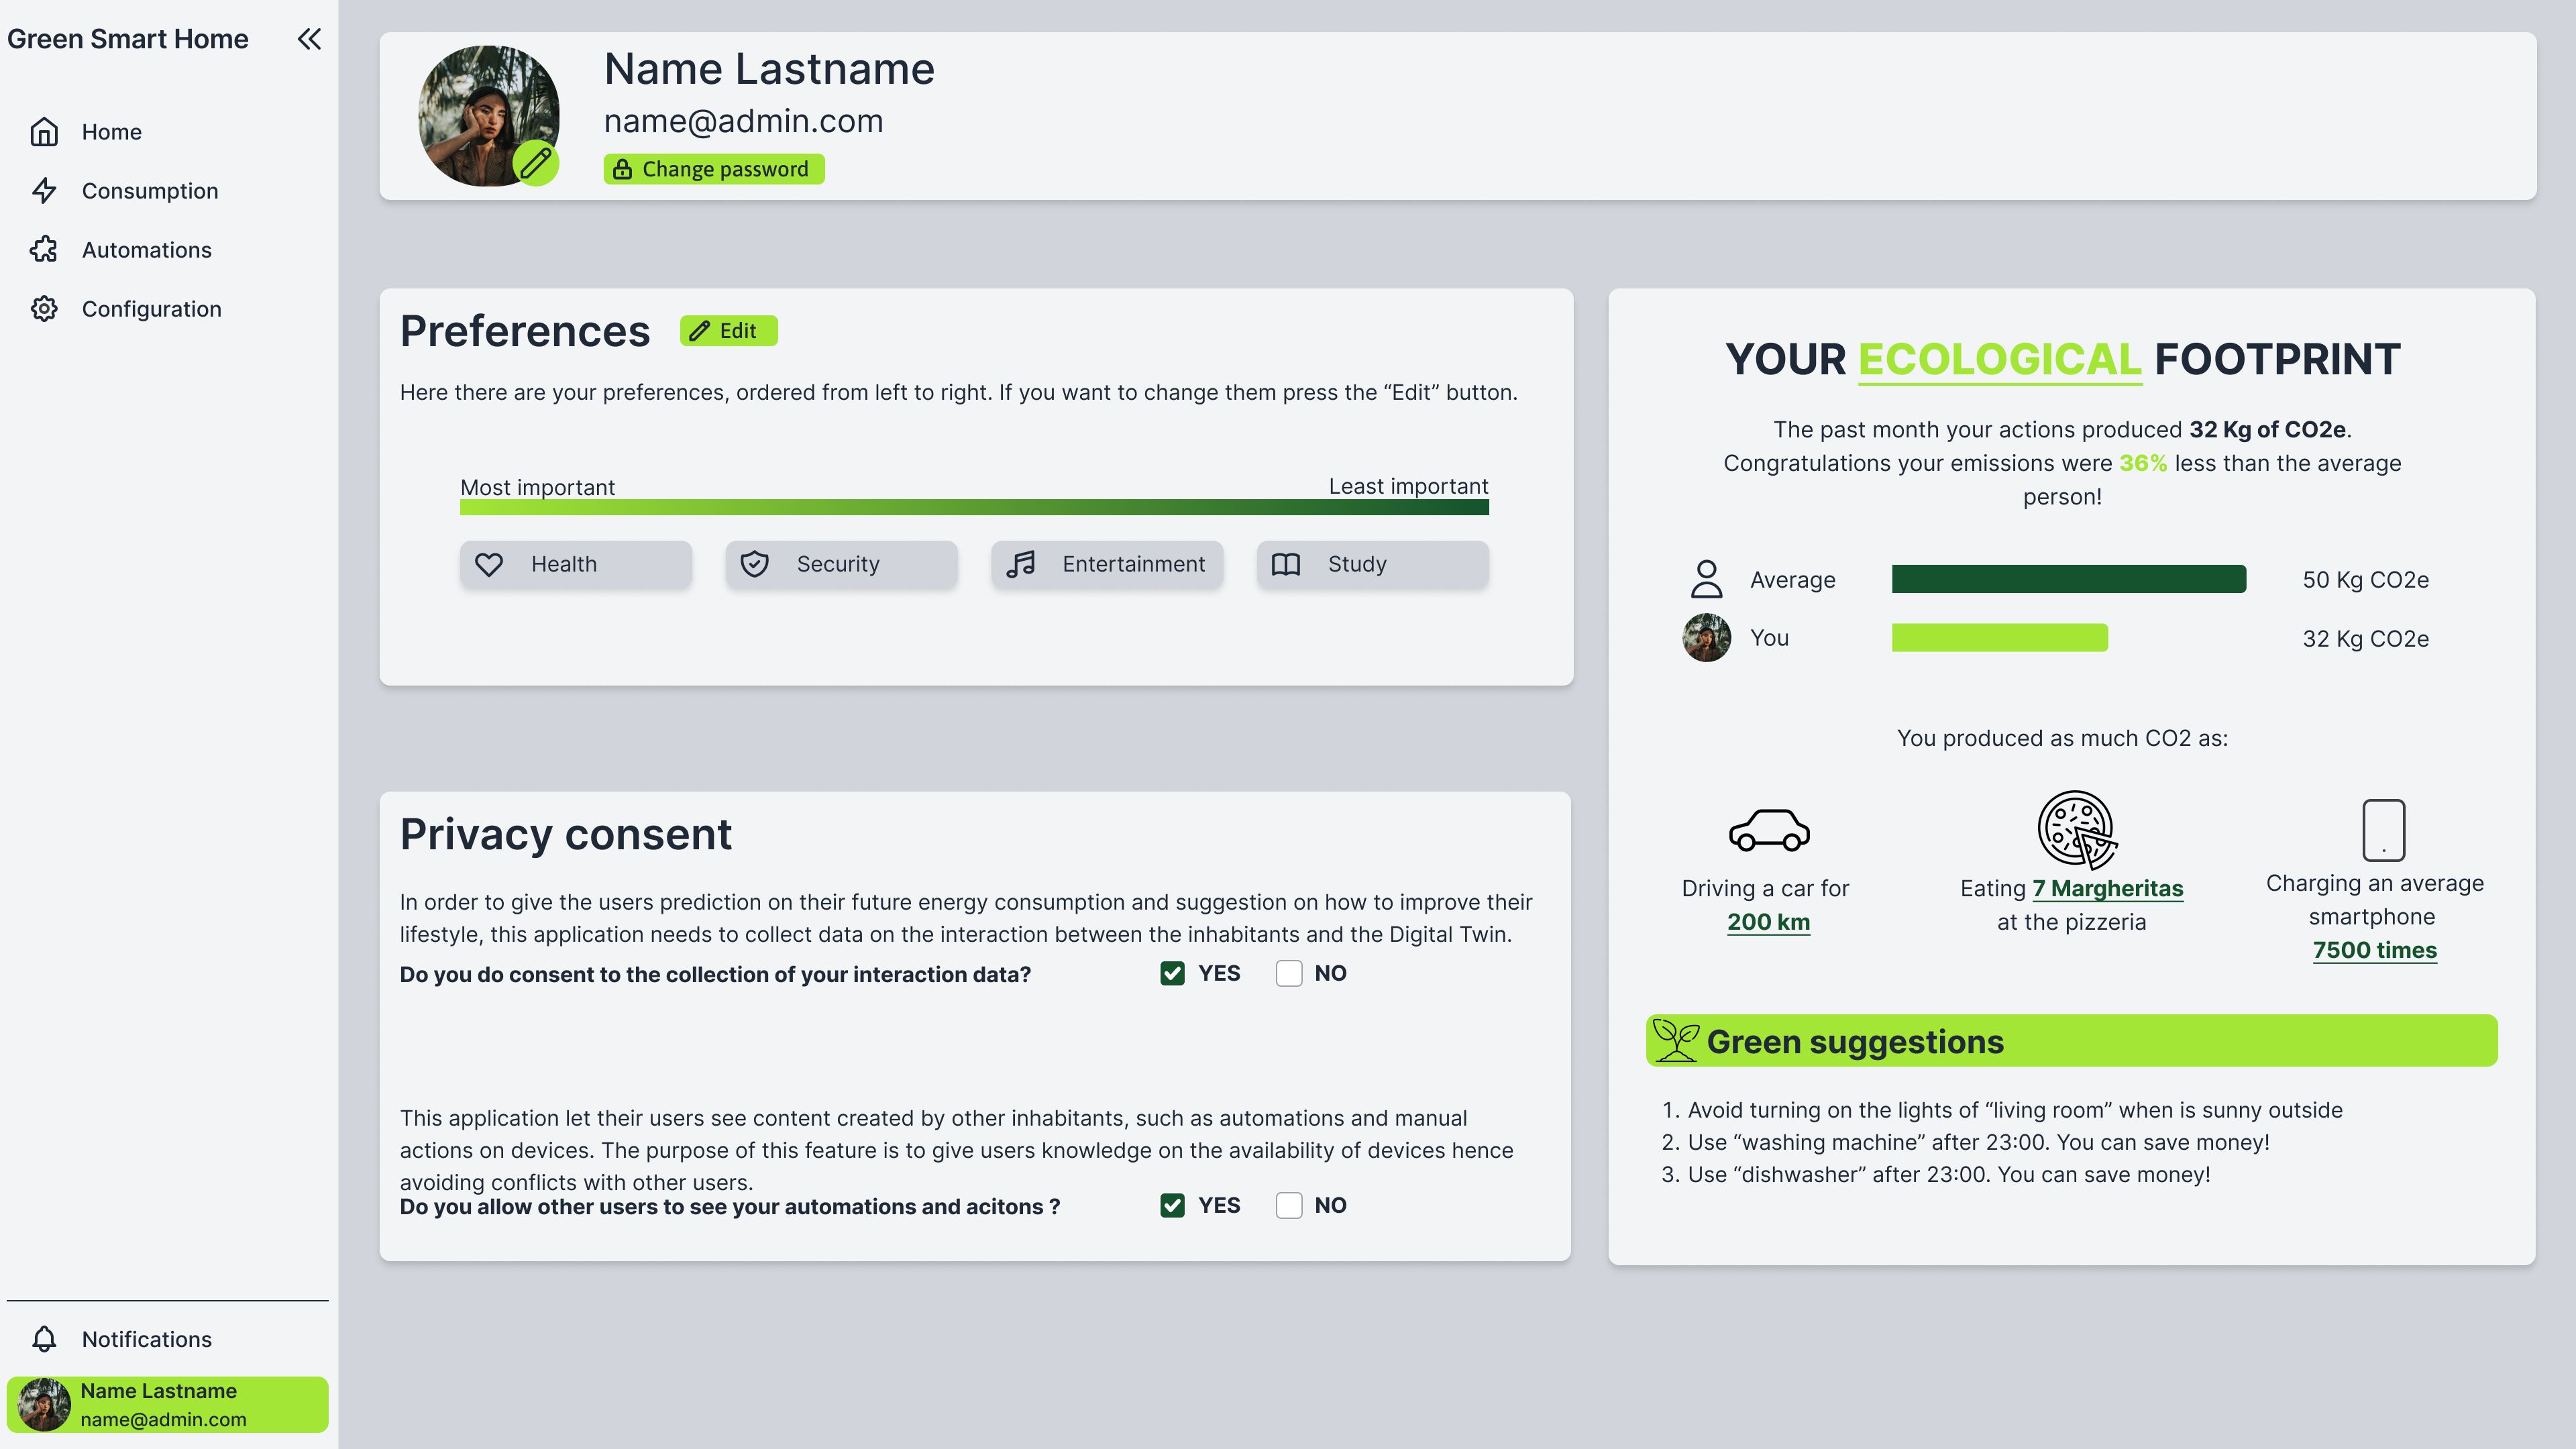
\includegraphics[width=1\linewidth]{images/Chap - 4/Profile.png}
    \caption{Sistema di partenza: area profilo con preferenze e privacy}
    \label{fig:cap4_base_profile}
\end{figure}

La vista specifica sull'impronta ecologica è mostrata in (fig.~\ref{fig:cap4_base_eco}), dove viene confrontato il profilo utente rispetto alla media e vengono proposti suggerimenti operativi.

\begin{figure}[H]
    \centering
    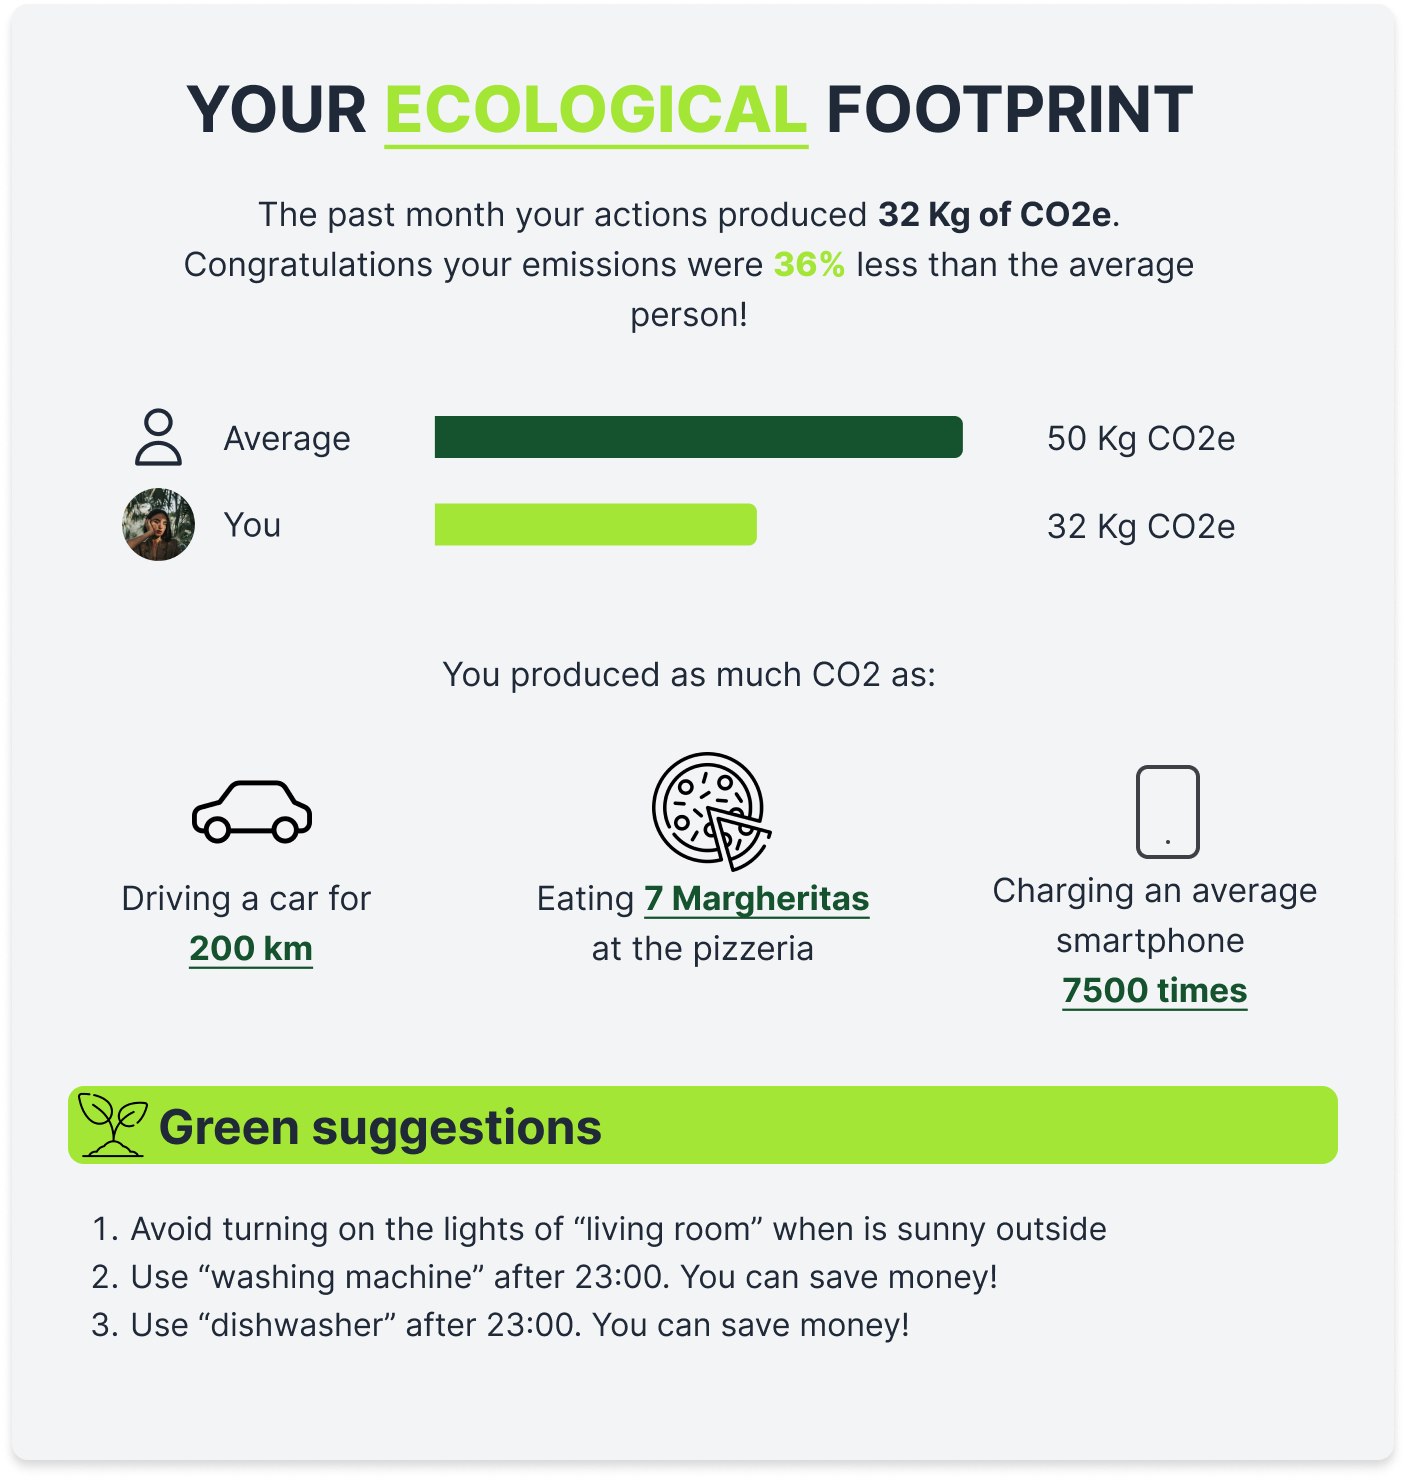
\includegraphics[width=0.8\linewidth]{images/Chap - 4/Ecological footprint.png}
    \caption{Sistema di partenza: dashboard dell'impronta ecologica}
    \label{fig:cap4_base_eco}
\end{figure}

Sono presenti anche componenti di \textit{engagement}, come il pop-up dedicato ad achievement e challenge (fig.~\ref{fig:cap4_base_achievements}).

\begin{figure}[H]
    \centering
    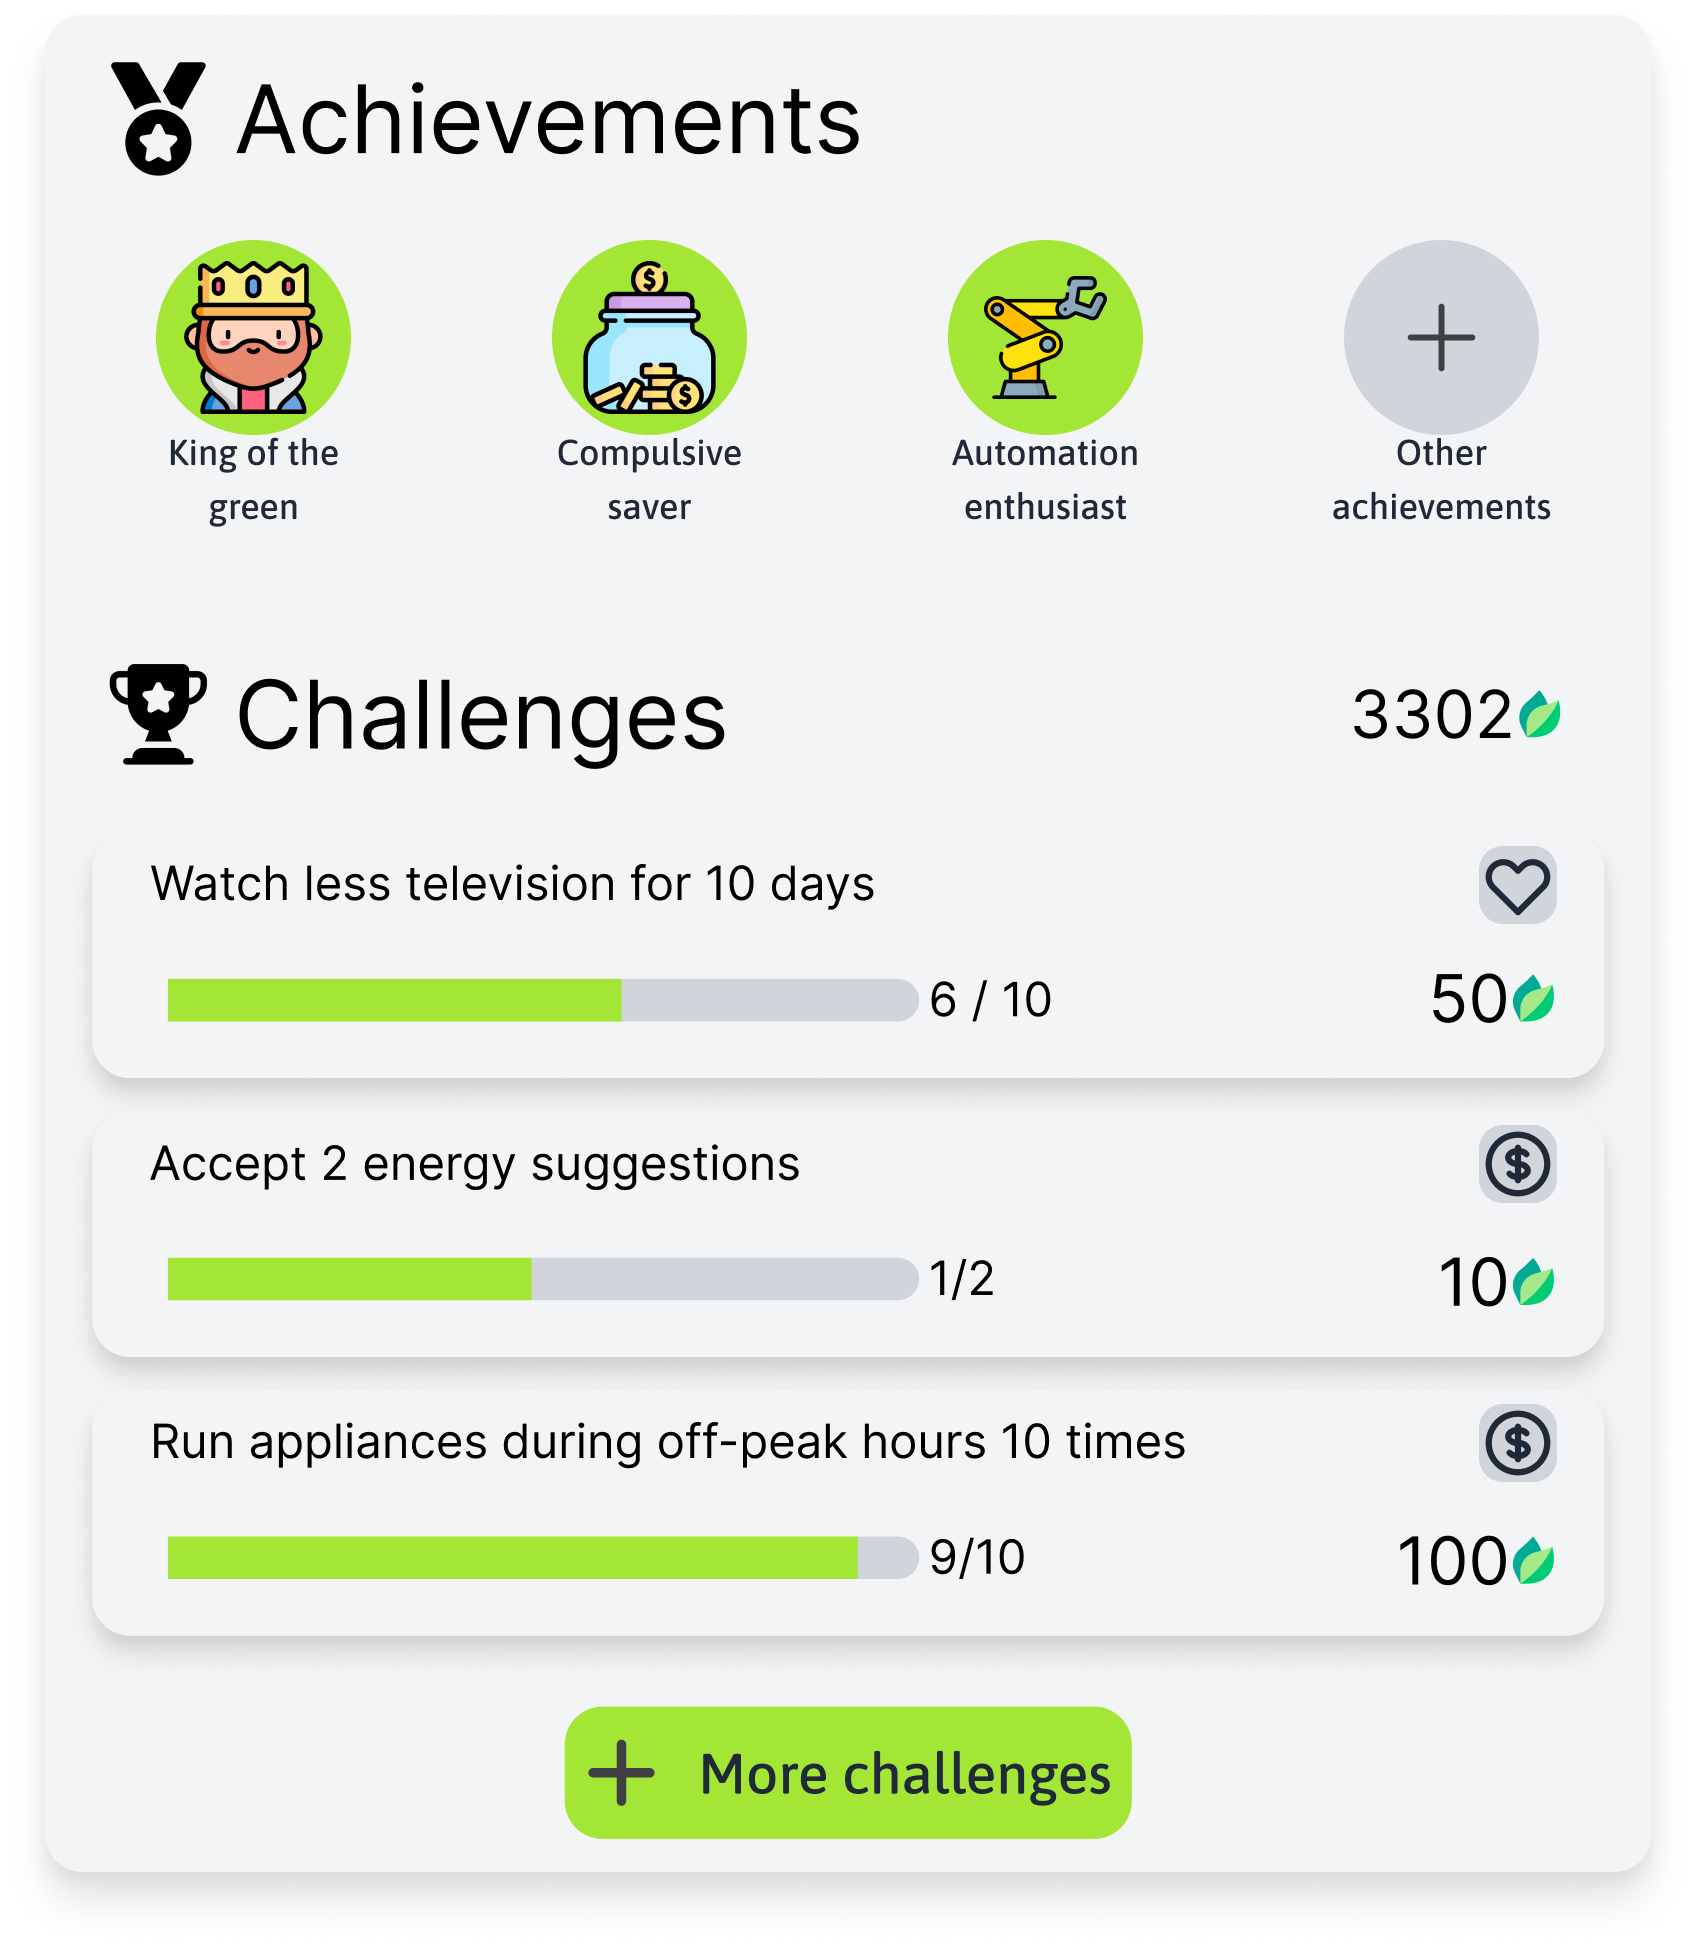
\includegraphics[width=0.5\linewidth]{images/Chap - 4/Achievements popup.png}
    \caption{Sistema di partenza: pop-up achievements e challenge}
    \label{fig:cap4_base_achievements}
\end{figure}

Per la gestione account sono disponibili modali dedicate al cambio password (fig.~\ref{fig:cap4_base_change_password}), cambio immagine profilo (fig.~\ref{fig:cap4_base_change_image}) e reset password (fig.~\ref{fig:cap4_base_reset_password}).

\begin{figure}[H]
    \centering
    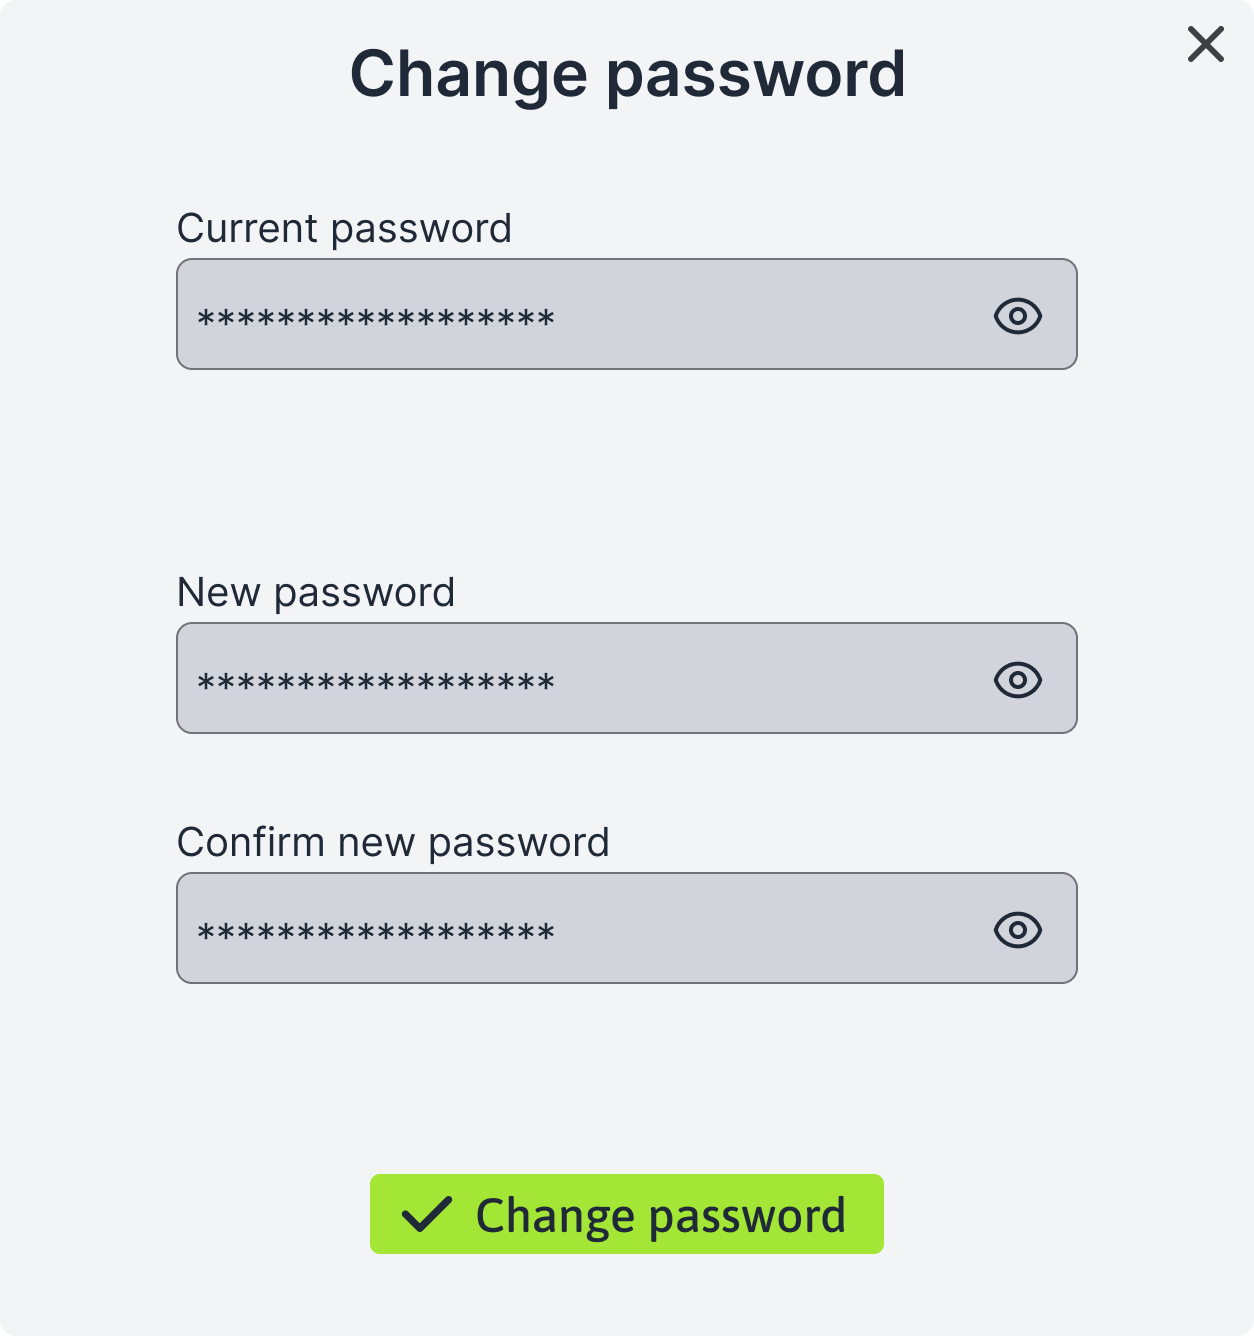
\includegraphics[width=0.65\linewidth]{images/Chap - 4/Change password popup.png}
    \caption{Sistema di partenza: modale cambio password}
    \label{fig:cap4_base_change_password}
\end{figure}

\begin{figure}[H]
    \centering
    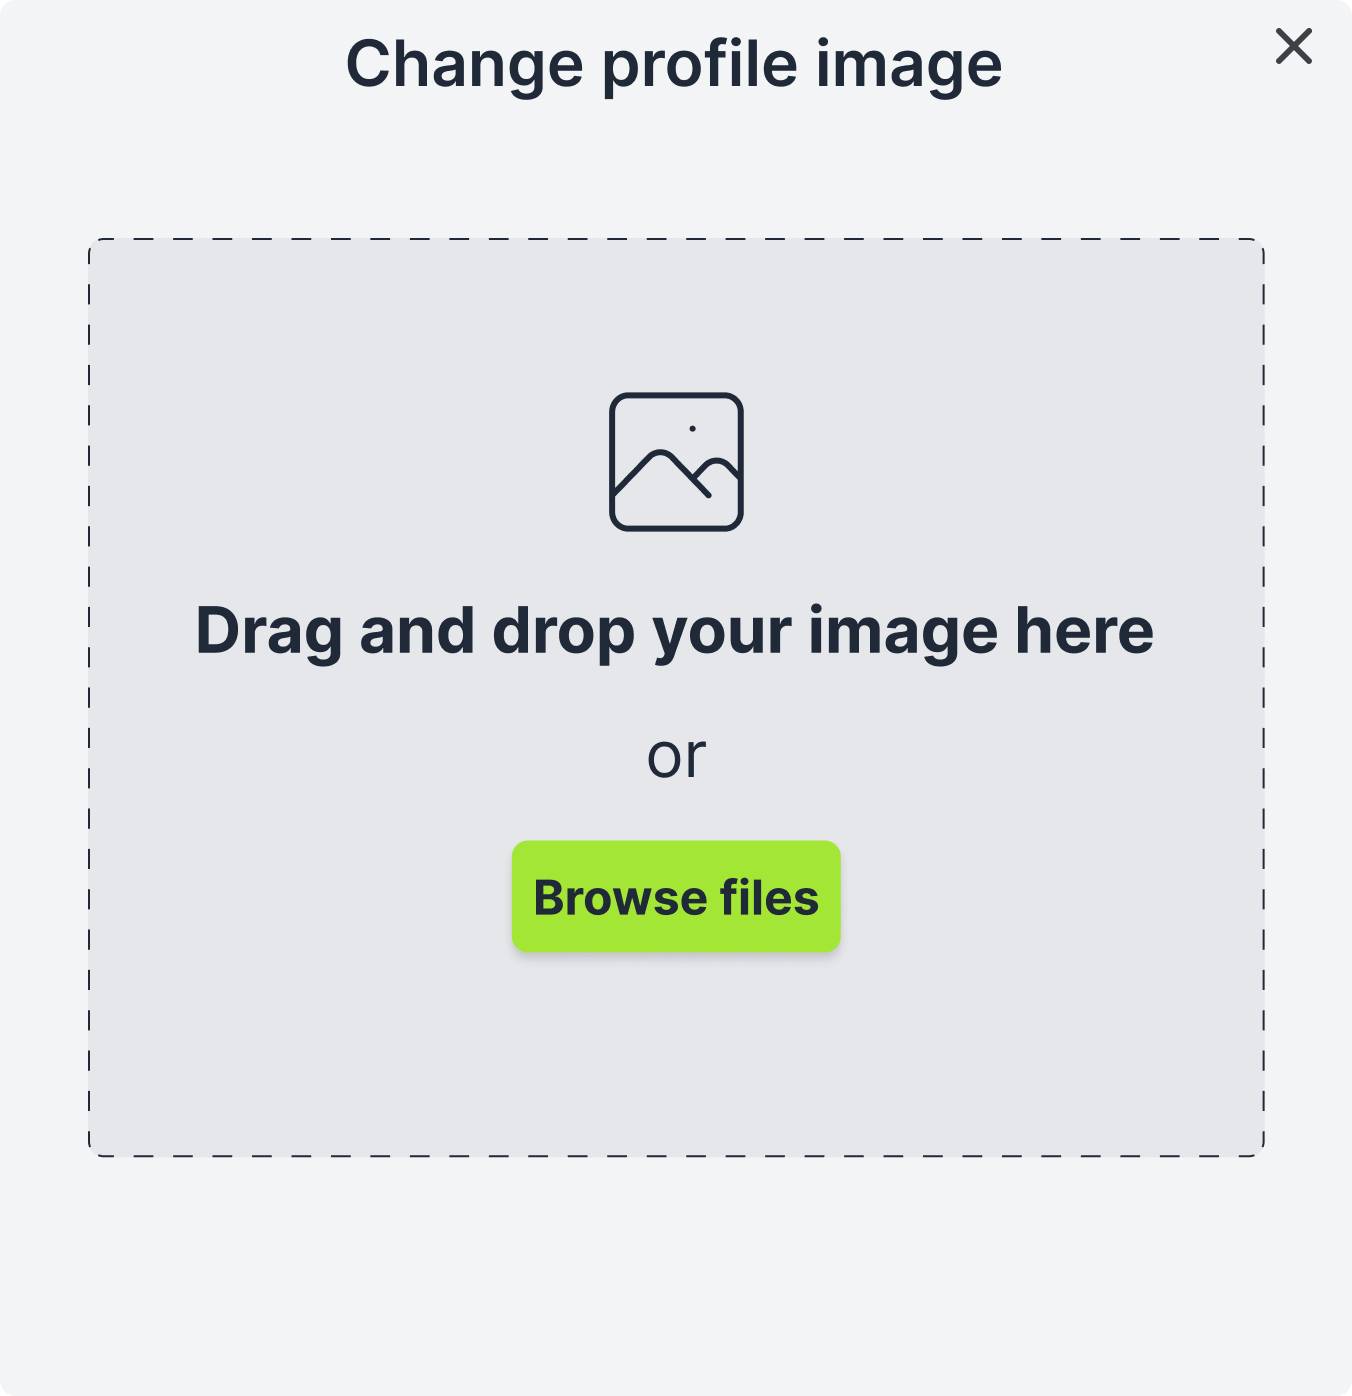
\includegraphics[width=0.65\linewidth]{images/Chap - 4/Profile image popup_1.png}
    \caption{Sistema di partenza: modale cambio immagine profilo}
    \label{fig:cap4_base_change_image}
\end{figure}

\begin{figure}[H]
    \centering
    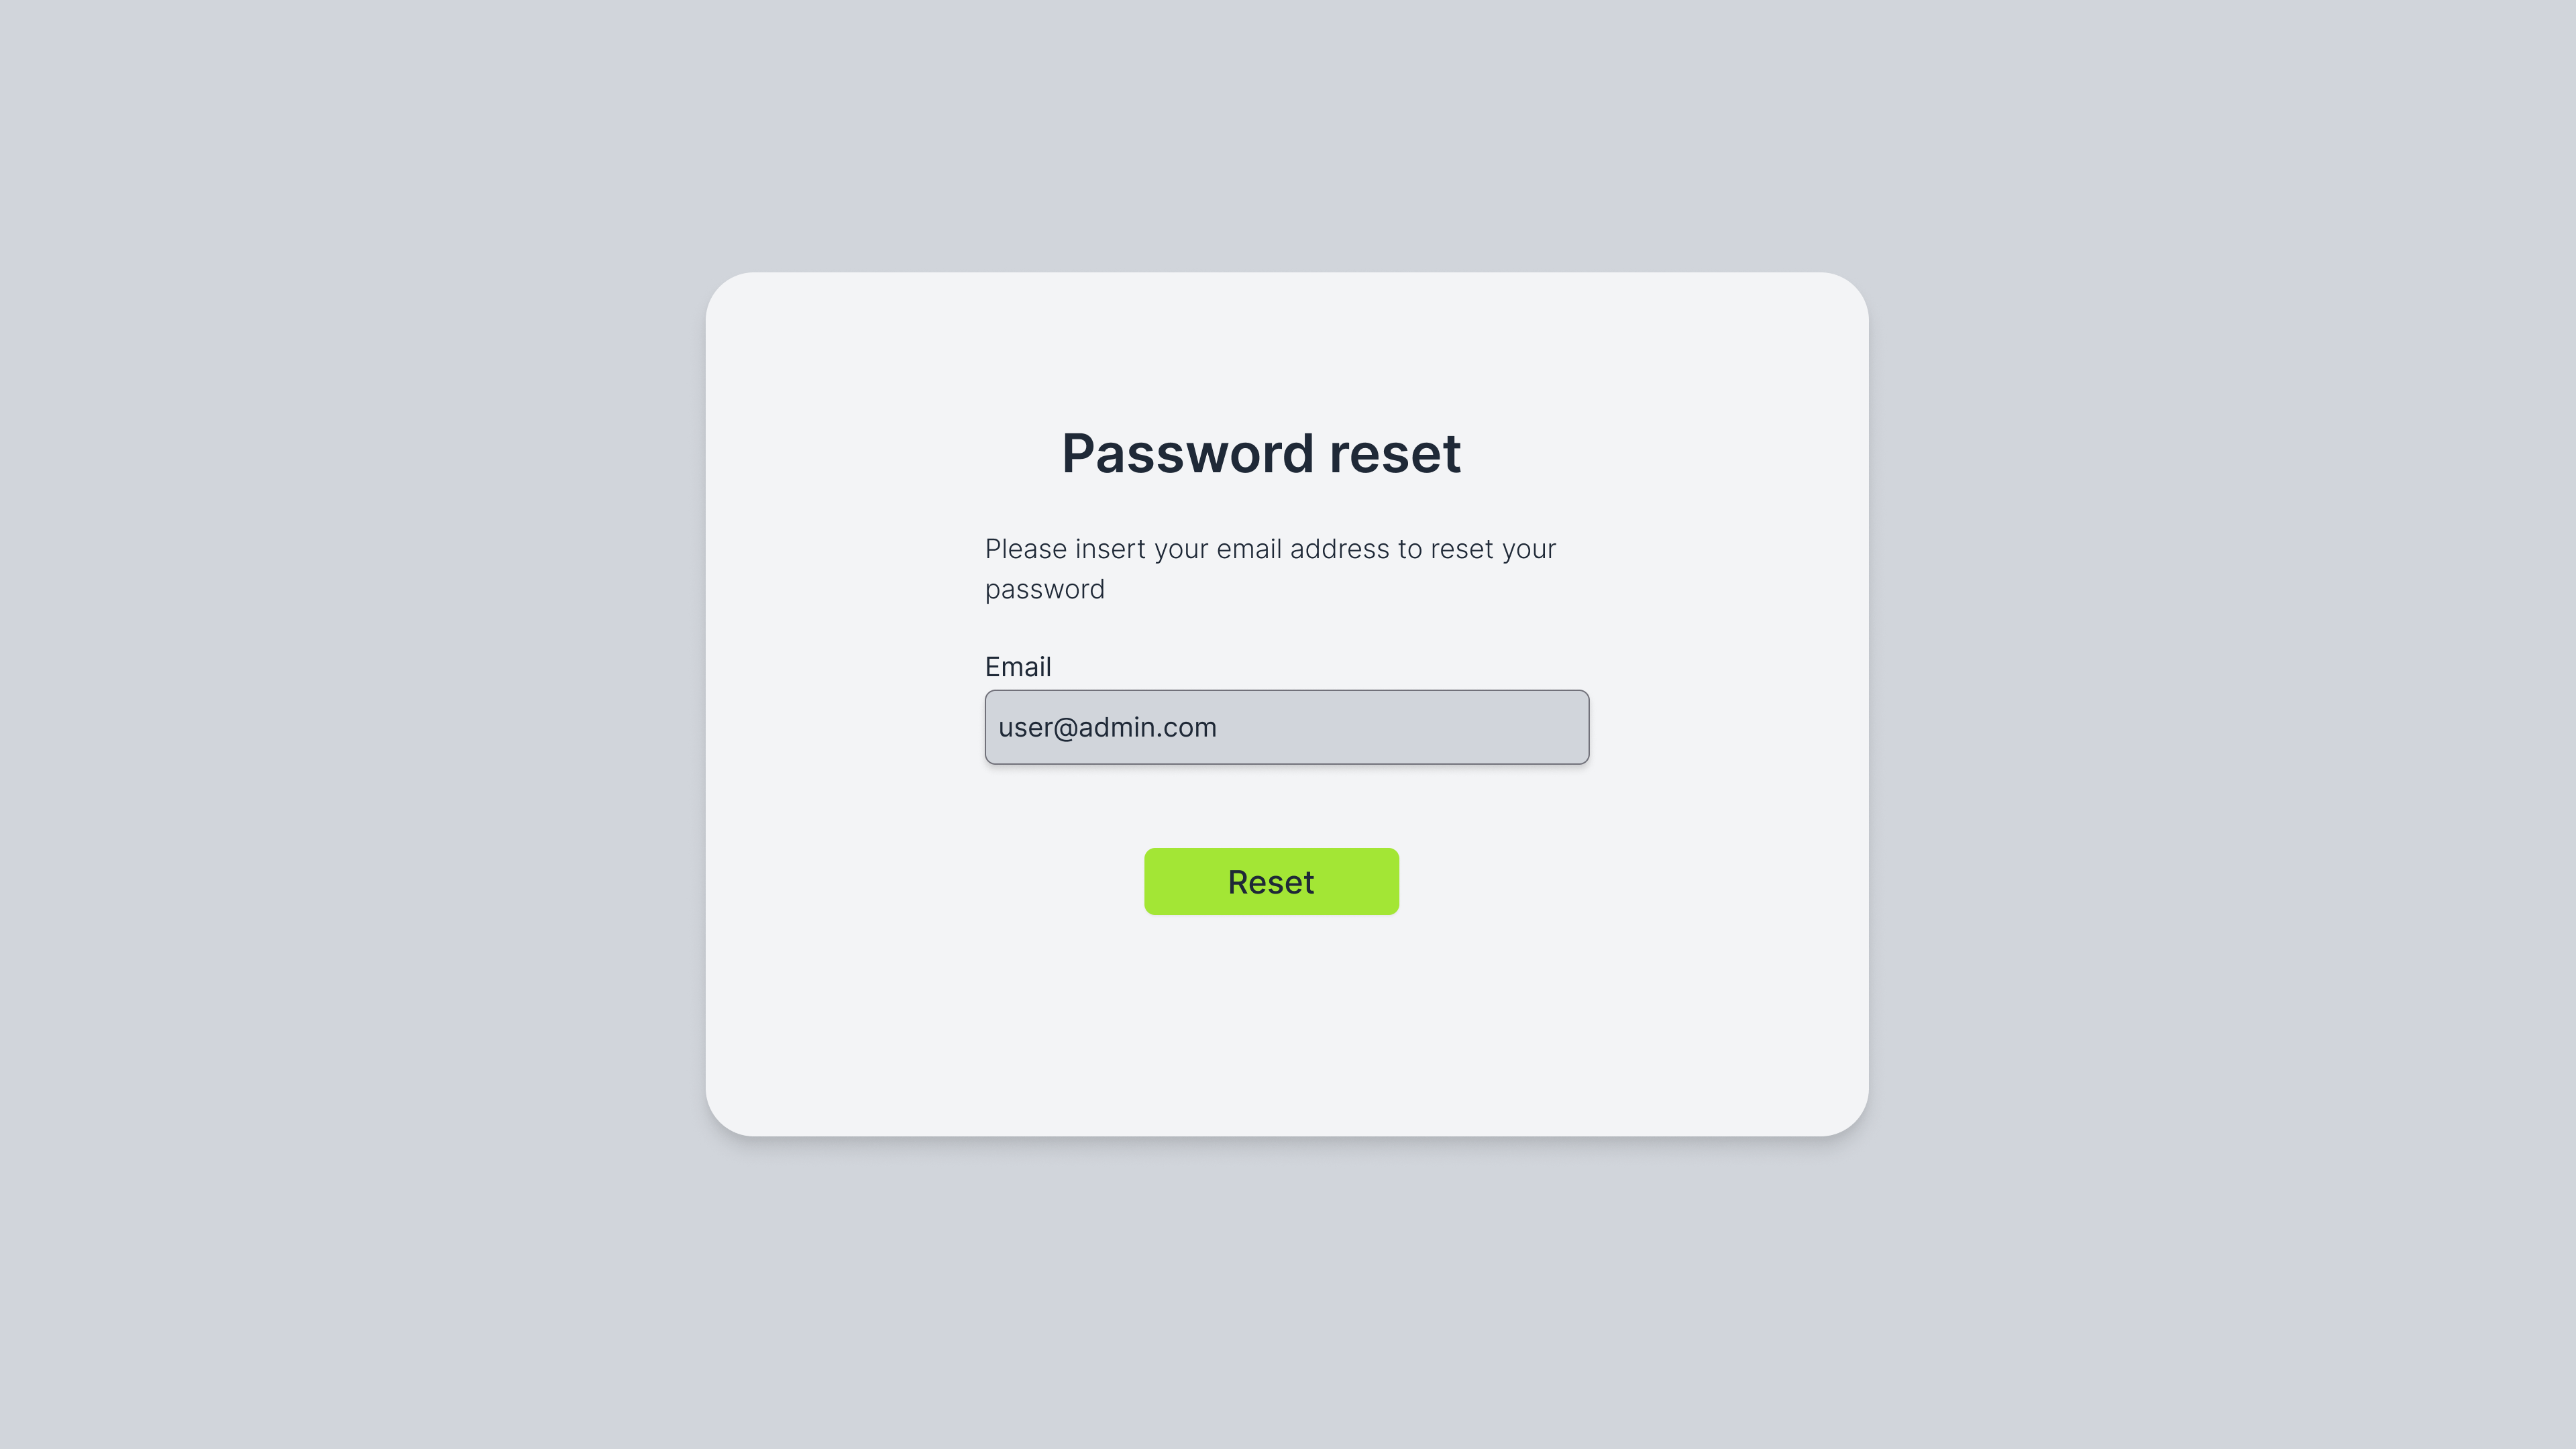
\includegraphics[width=0.75\linewidth]{images/Chap - 4/Password reset.png}
    \caption{Sistema di partenza: schermata di reset password}
    \label{fig:cap4_base_reset_password}
\end{figure}

Inoltre il sistema integra schermate di supporto predittivo direttamente su singolo dispositivo, come nel caso dell'aria condizionata e della lavatrice mostrati in (fig.~\ref{fig:cap4_base_prediction_cotton}) e (fig.~\ref{fig:cap4_base_prediction_express}).

\begin{figure}[H]
    \centering
    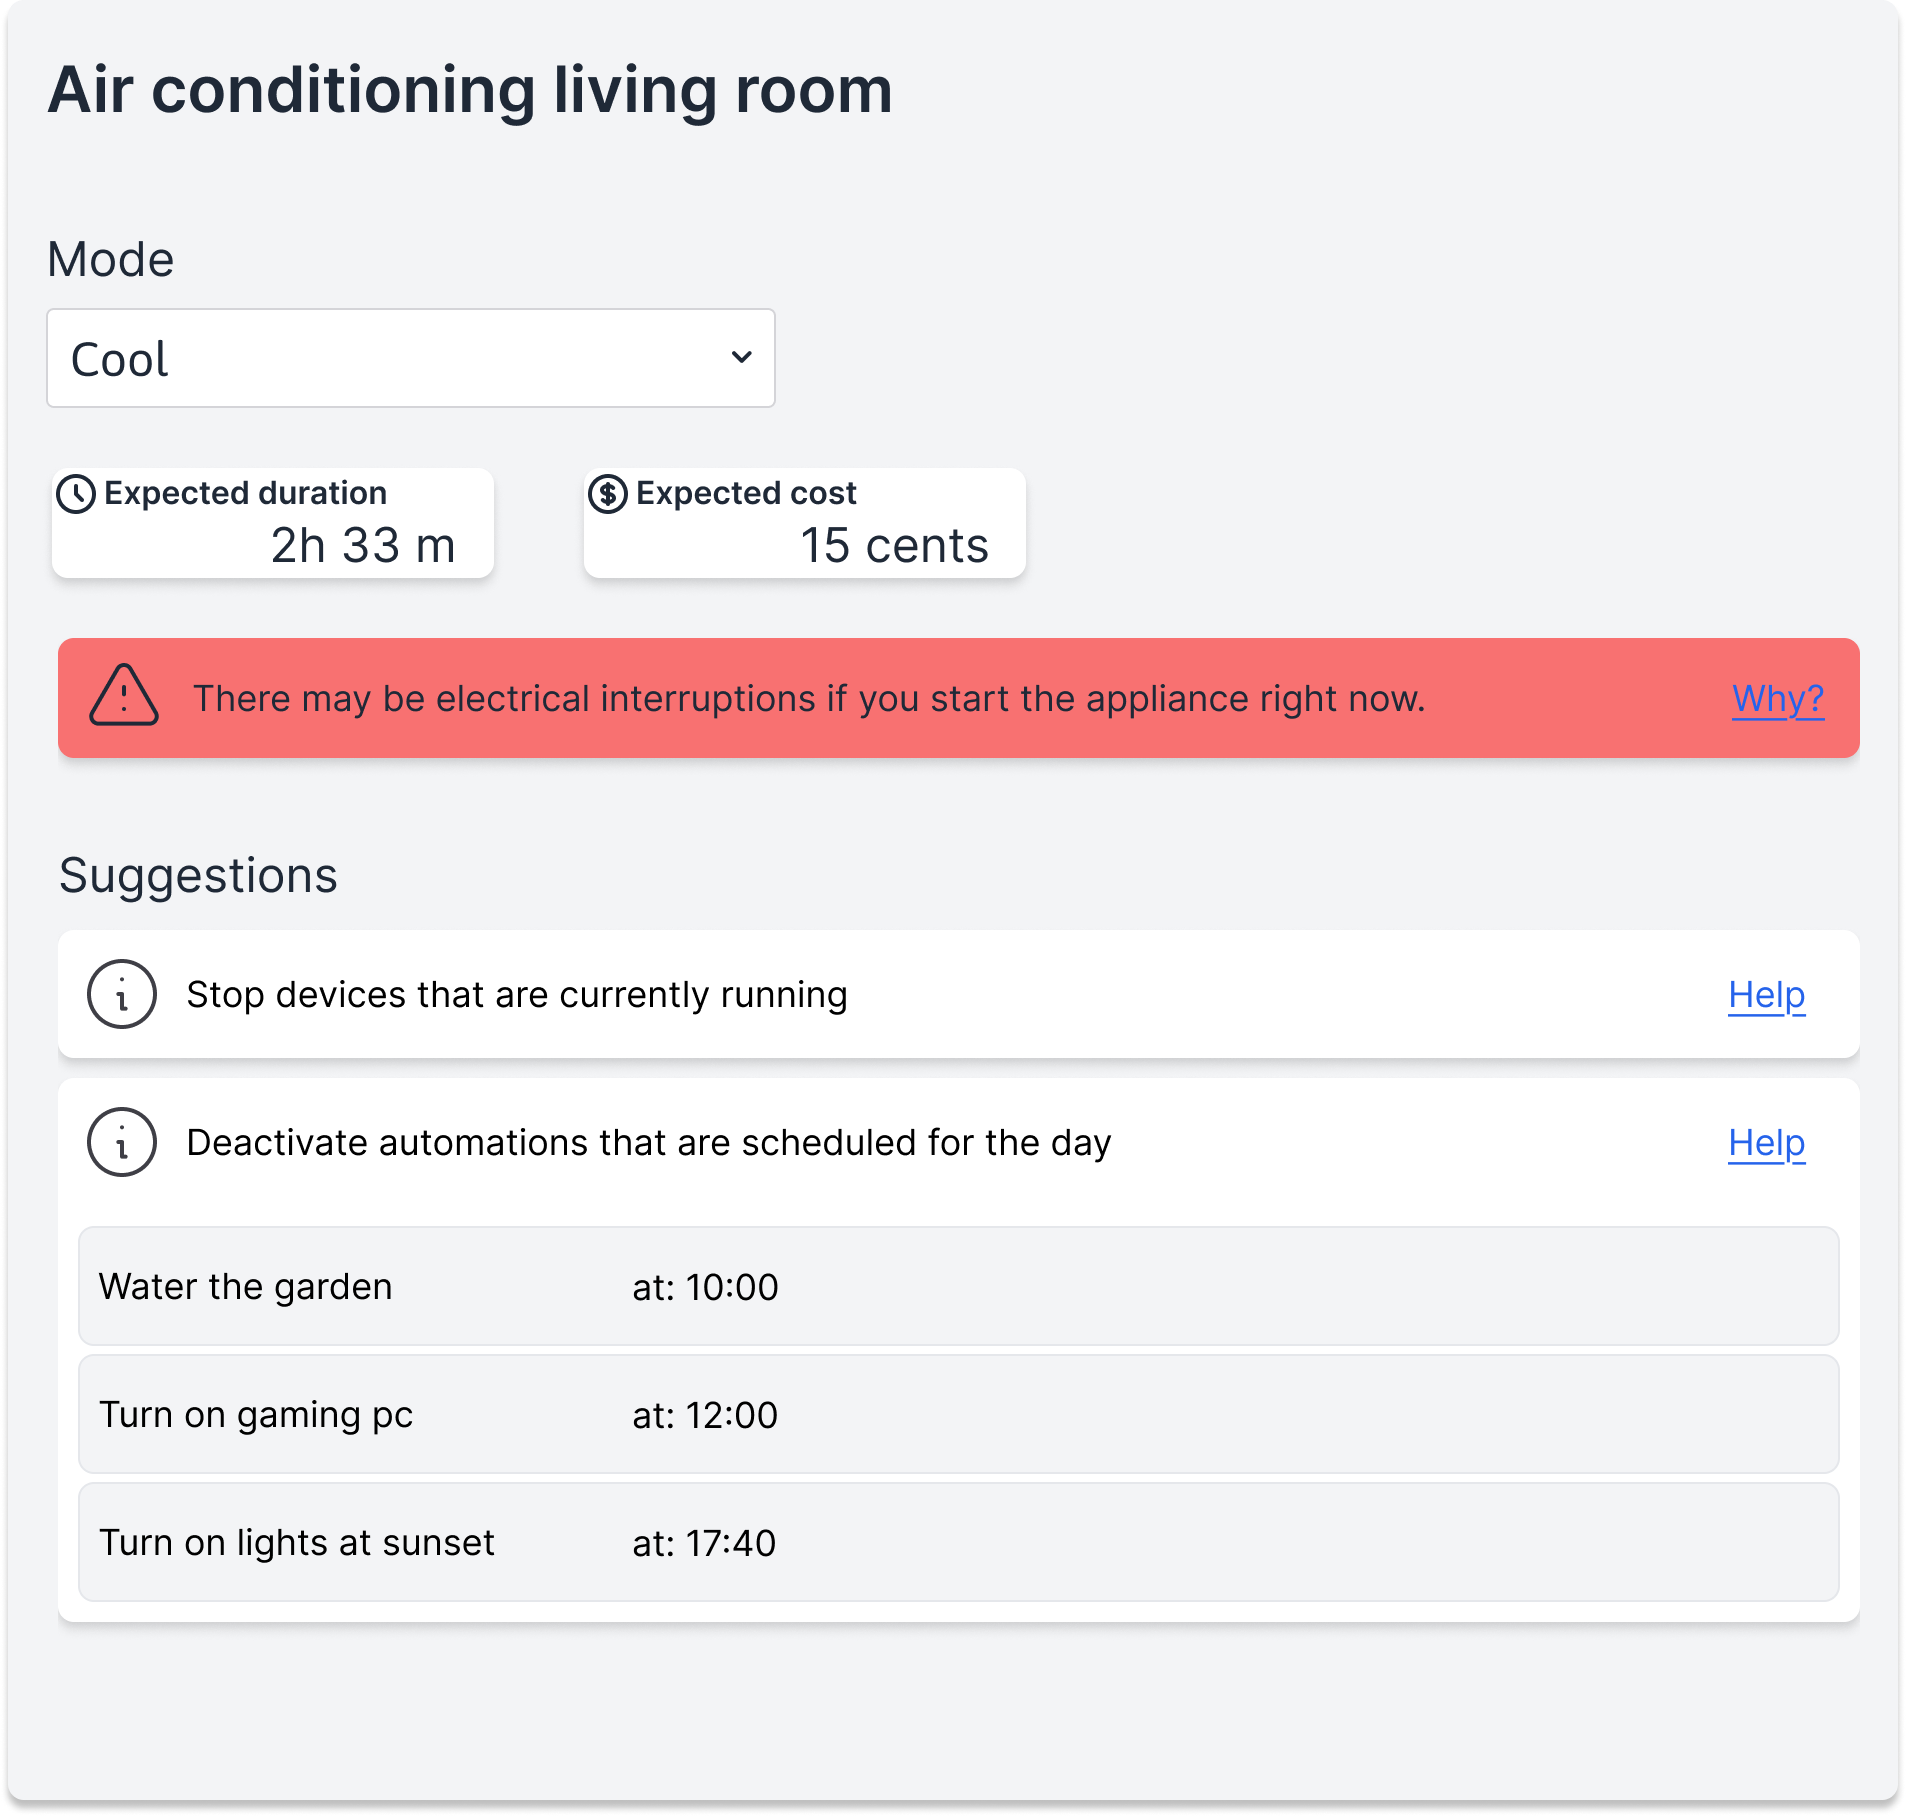
\includegraphics[width=0.85\linewidth]{images/Chap - 4/Step=Prediction, Mode=Cotton.png}
    \caption{Sistema di partenza: schermata predittiva su dispositivo (esempio 1)}
    \label{fig:cap4_base_prediction_cotton}
\end{figure}

\begin{figure}[H]
    \centering
    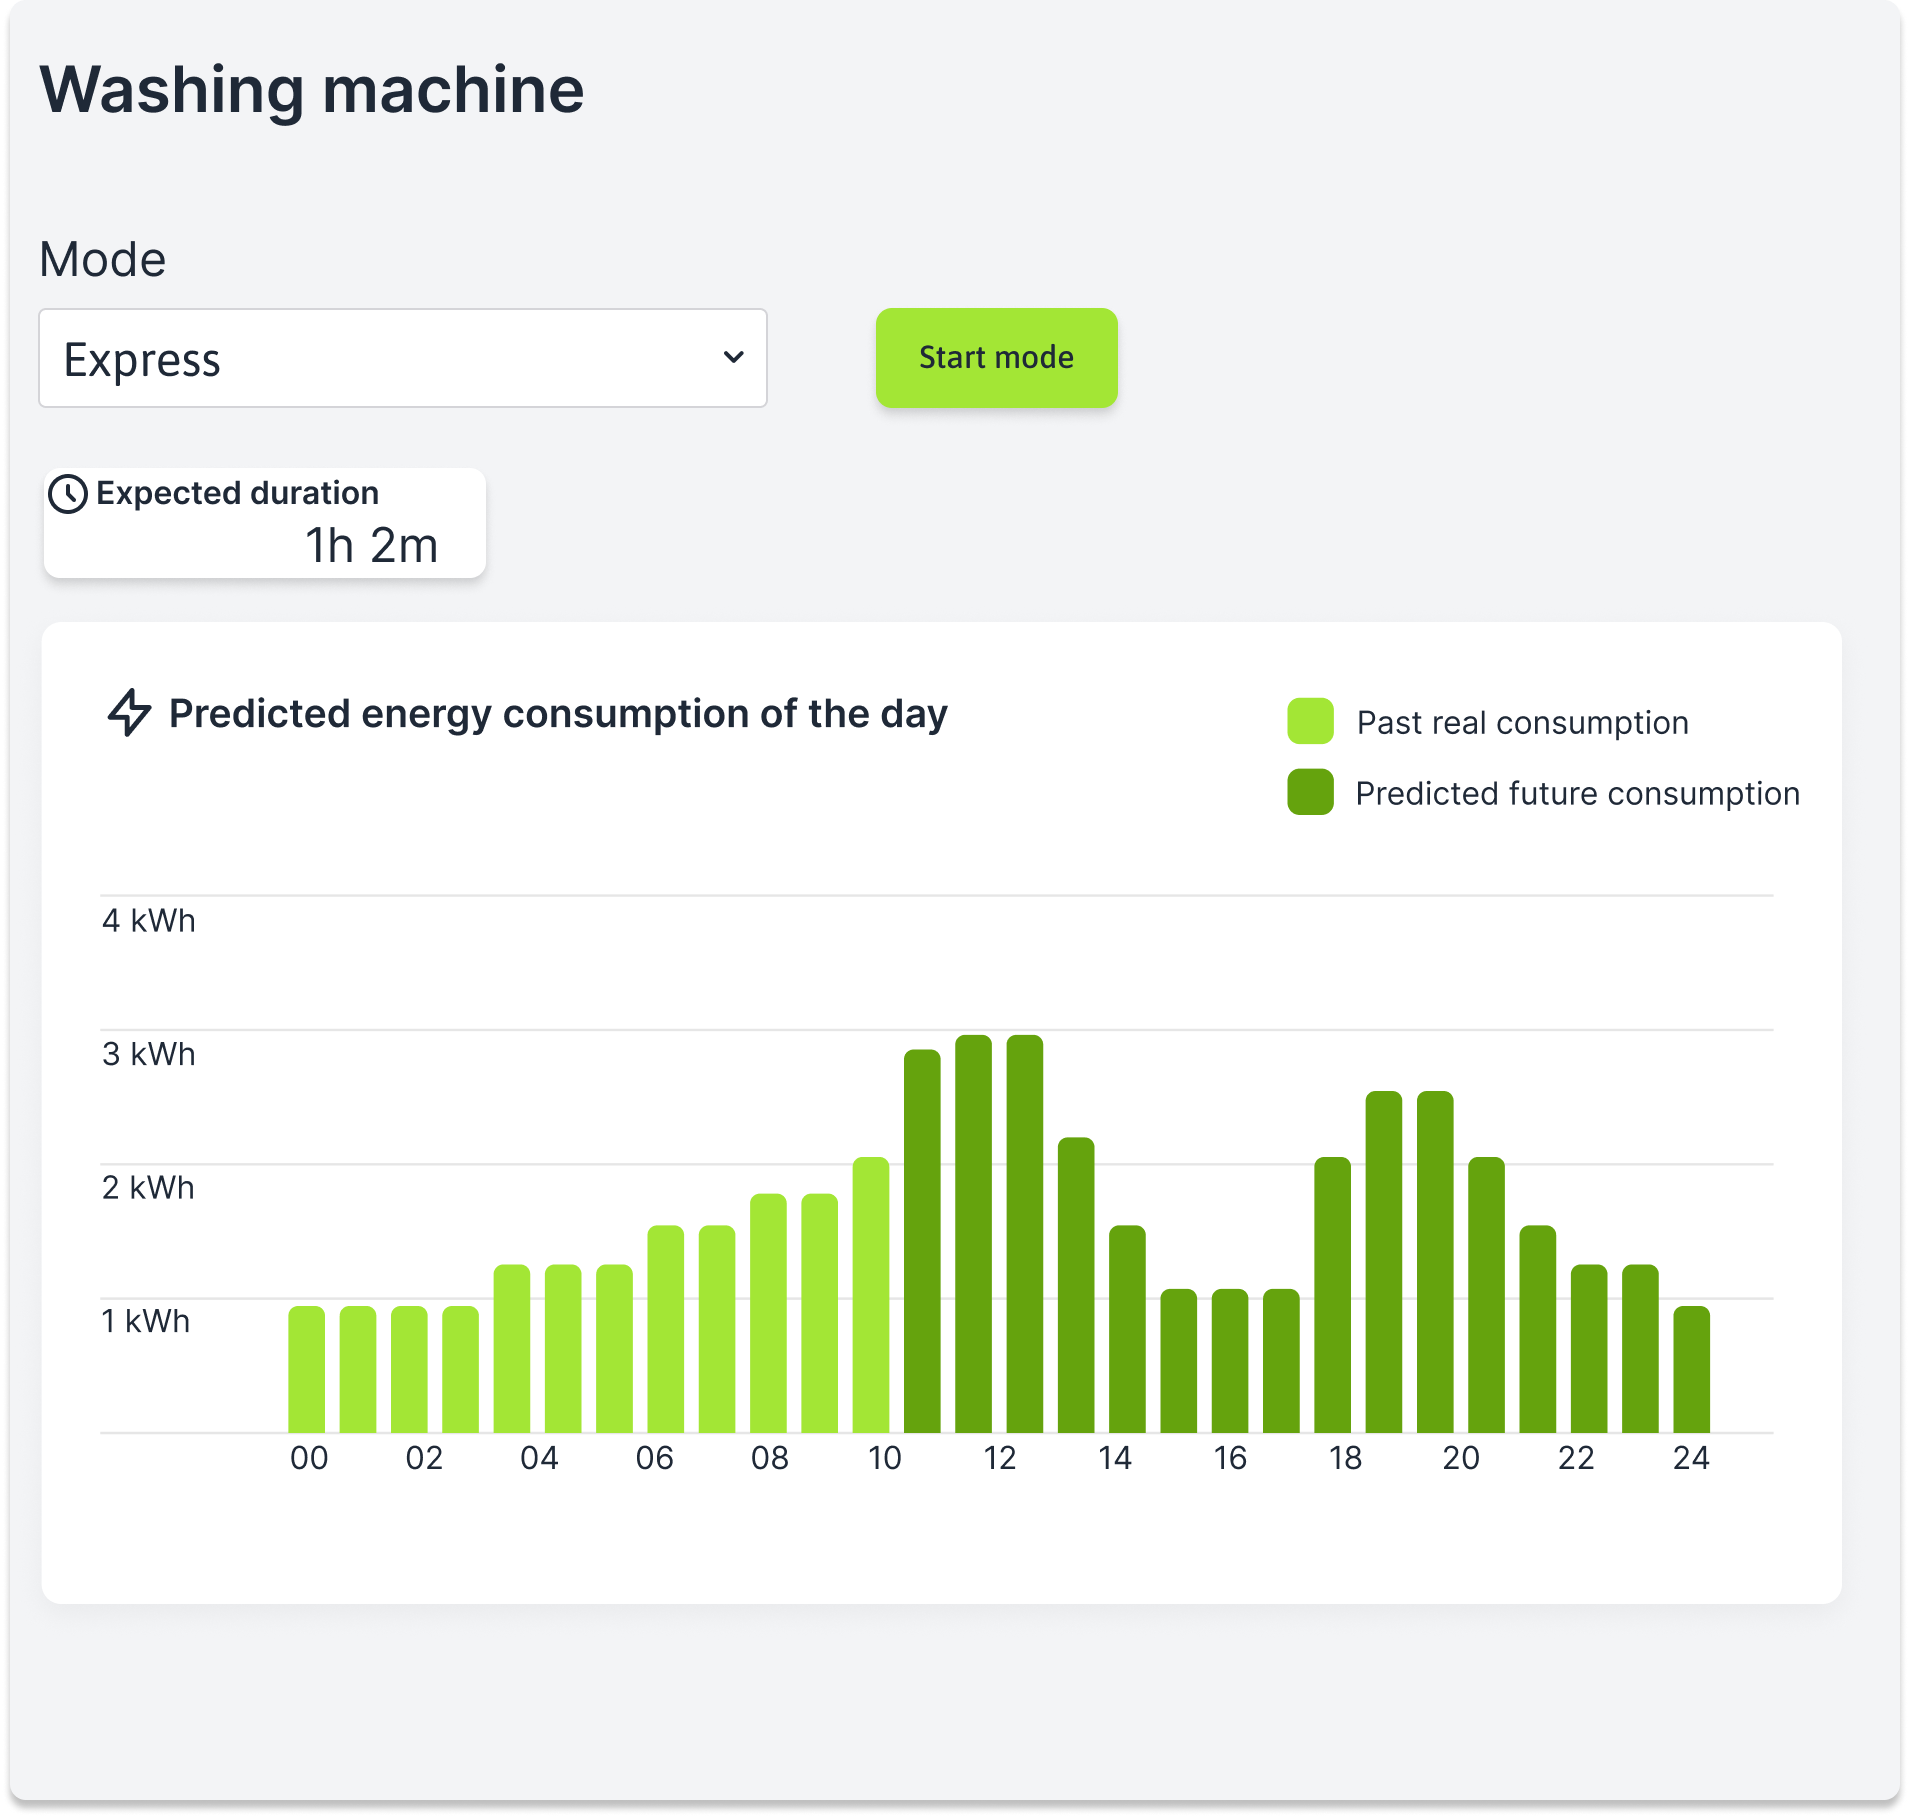
\includegraphics[width=0.85\linewidth]{images/Chap - 4/Step=Prediction, Mode=Expres.png}
    \caption{Sistema di partenza: schermata predittiva su dispositivo (esempio 2)}
    \label{fig:cap4_base_prediction_express}
\end{figure}

Infine, la palette colori definita nel prototipo iniziale è riportata in (fig.~\ref{fig:cap4_base_palette}), con distinzione tra colori testuali, colori di superficie e colori di accento.

\begin{figure}[H]
    \centering
    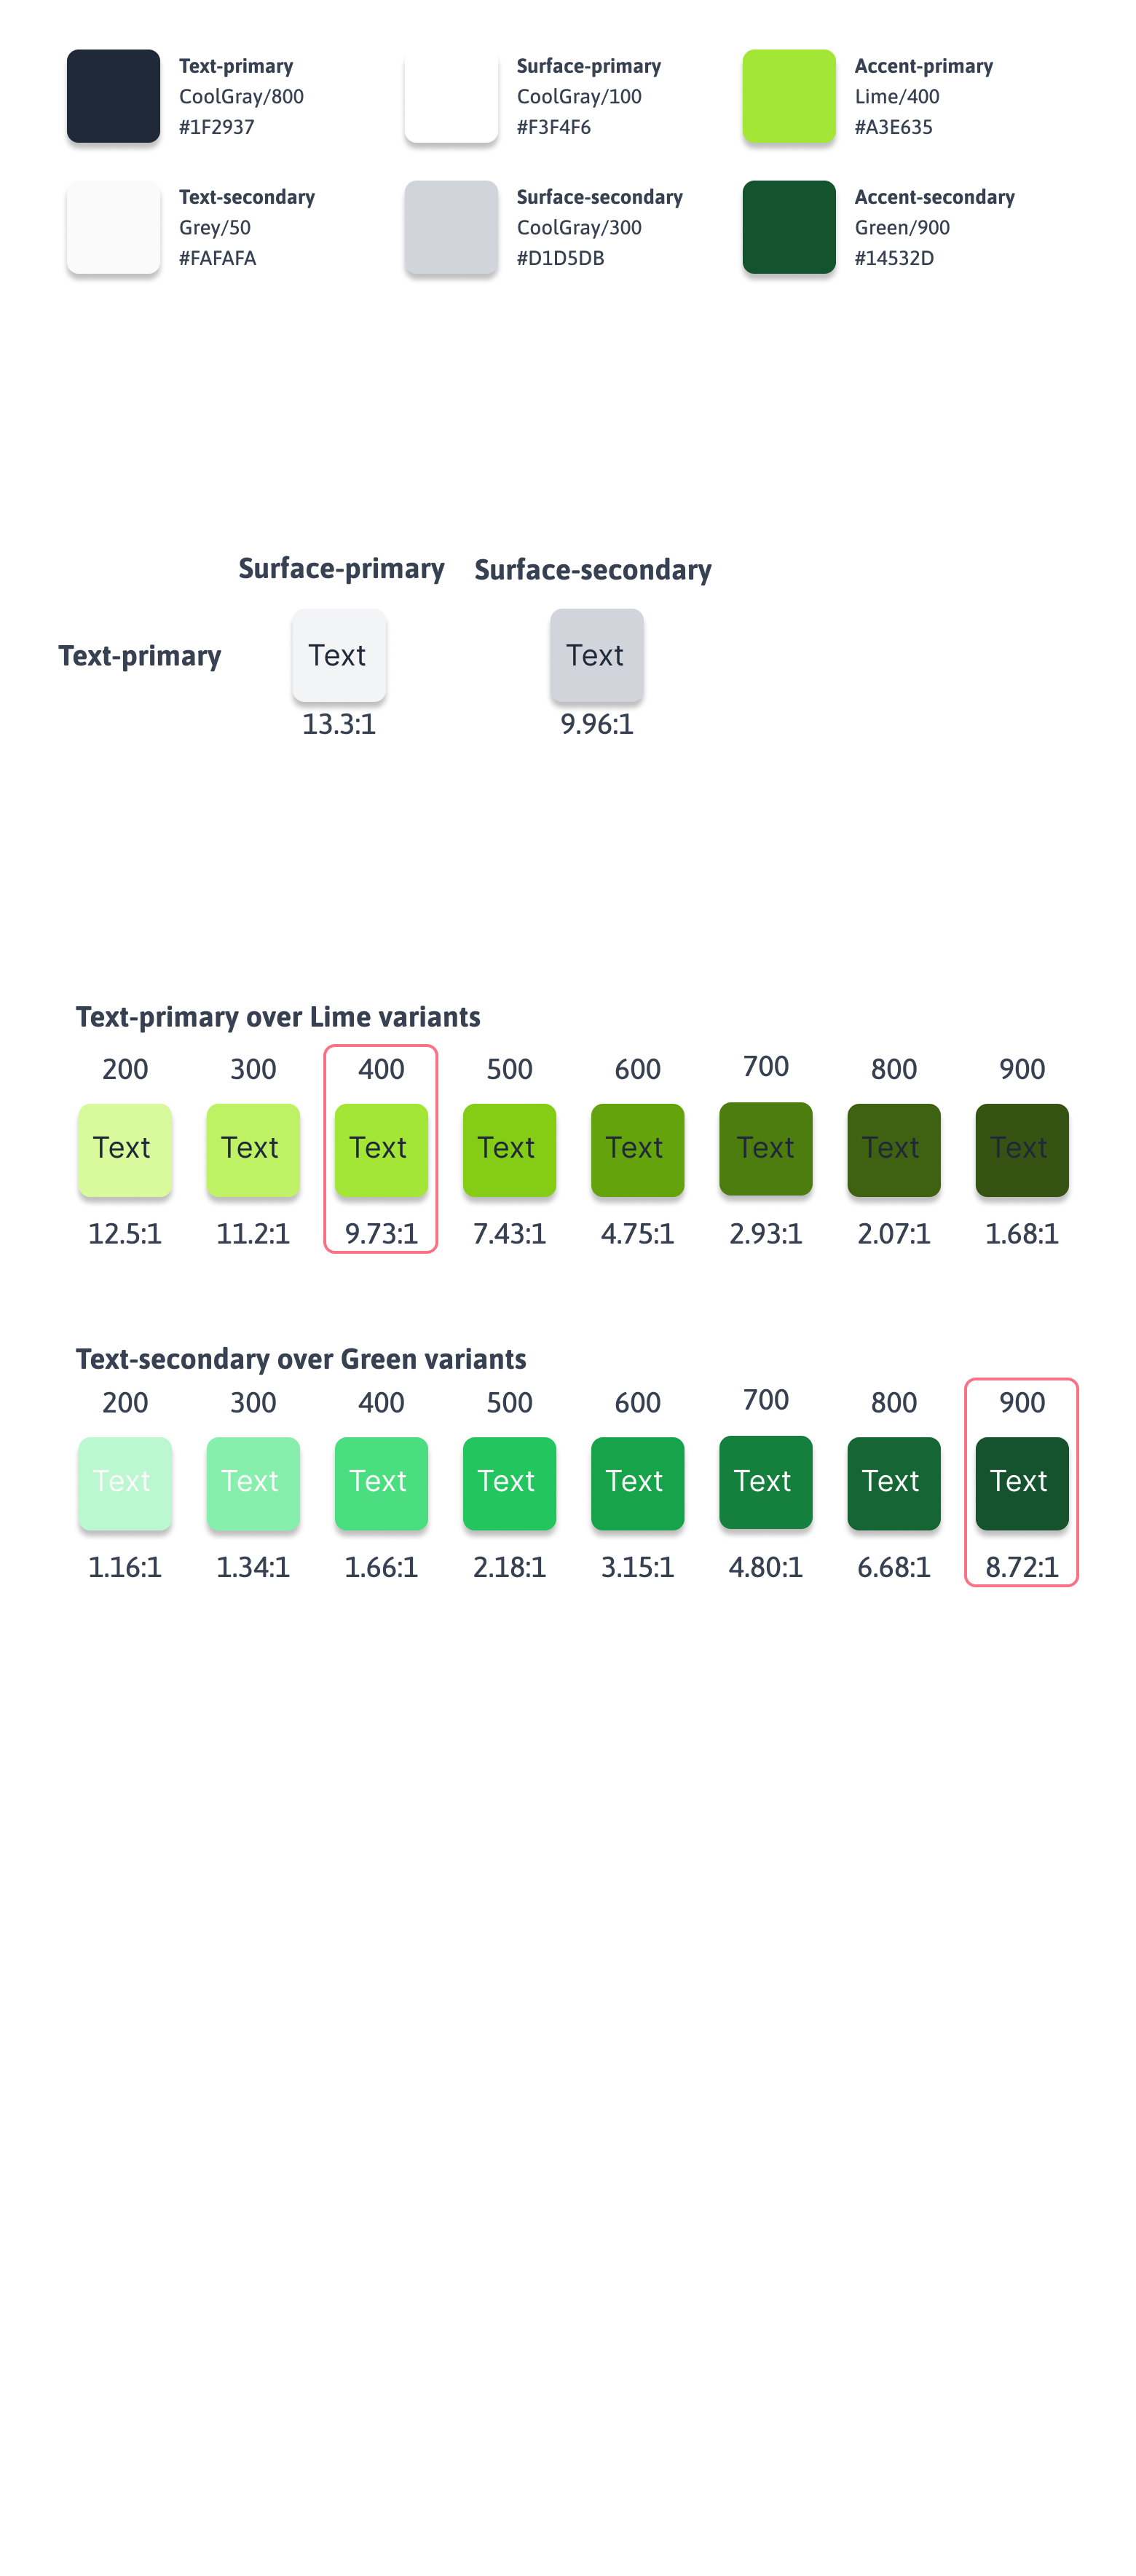
\includegraphics[width=0.5\linewidth]{images/Chap - 4/Color palette.png}
    \caption{Sistema di partenza: palette grafica utilizzata}
    \label{fig:cap4_base_palette}
\end{figure}

\section{Limiti osservati nel sistema di partenza}
Dall'analisi complessiva emerge che il sistema di partenza è ricco nelle funzioni di monitoraggio e configurazione, ma presenta un limite importante nella parte TAP: l'utente può soprattutto visualizzare e gestire automazioni già presenti, mentre non ha ancora un flusso completo e guidato per creare una nuova automazione da zero dentro la stessa interfaccia.

Questo punto è coerente con quanto discusso nel Capitolo~\ref{chap:digital-twin-smart-home}, dove la creazione delle automazioni era ancora fortemente legata a strumenti esterni o a processi separati rispetto alla GUI principale del Gemello Digitale.

\section{Il mio sviluppo: integrazione del builder TAP nella GUI}
Per superare il limite precedente, ho progettato una nuova sezione di creazione automazioni direttamente all'interno della pagina \textit{Automations}. Le schermate del mio sviluppo sono riportate nelle immagini presenti in \texttt{images/Chap - 4/GOLINO}.

La prima schermata (fig.~\ref{fig:cap4_golino_builder_top}) mostra la struttura generale del builder: nella parte centrale è presente il form per definire le condizioni di attivazione (\textit{When}) e nella parte destra il riepilogo in linguaggio naturale della regola che si sta creando.

\begin{figure}[H]
    \centering
    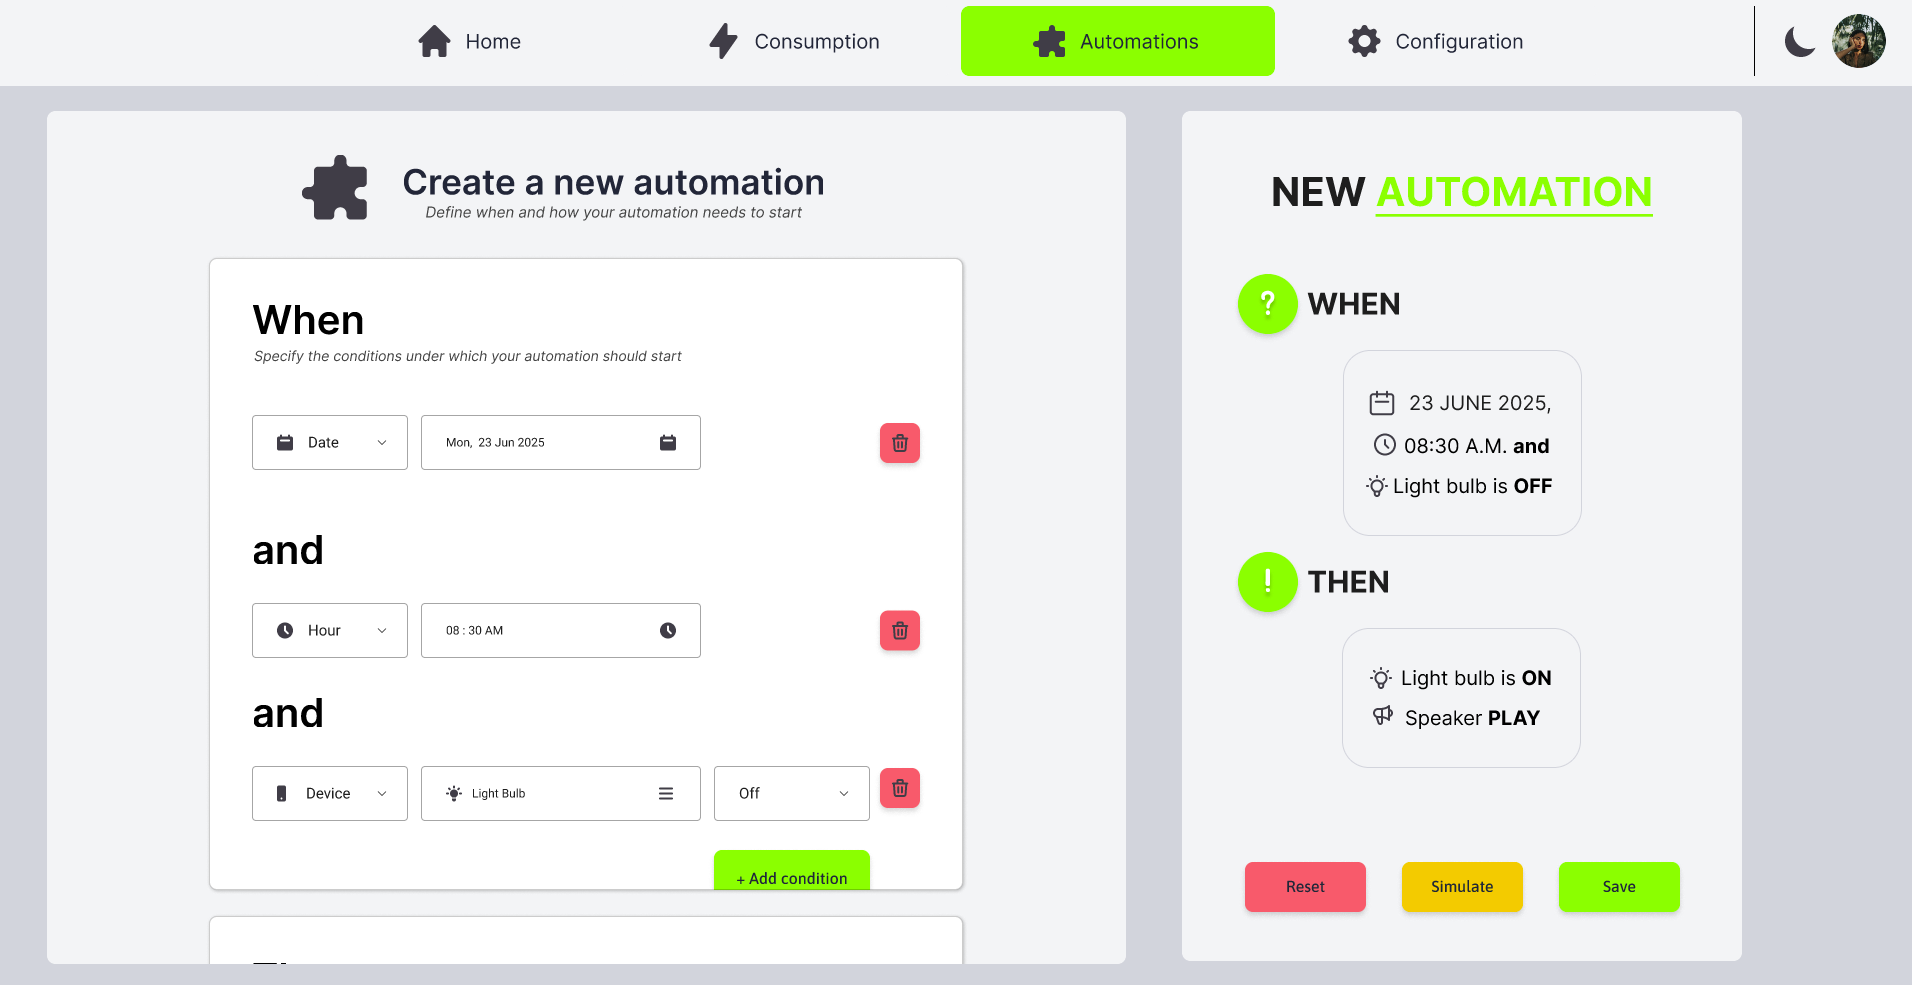
\includegraphics[width=1\linewidth]{images/Chap - 4/GOLINO/figma - UI Golino.png}
    \caption{Mio sviluppo: nuova interfaccia per la creazione di automazioni (parte alta)}
    \label{fig:cap4_golino_builder_top}
\end{figure}

La seconda schermata (fig.~\ref{fig:cap4_golino_builder_bottom}) completa il flusso introducendo la sezione \textit{Then}, quindi le azioni da eseguire quando le condizioni sono soddisfatte.

\begin{figure}[H]
    \centering
    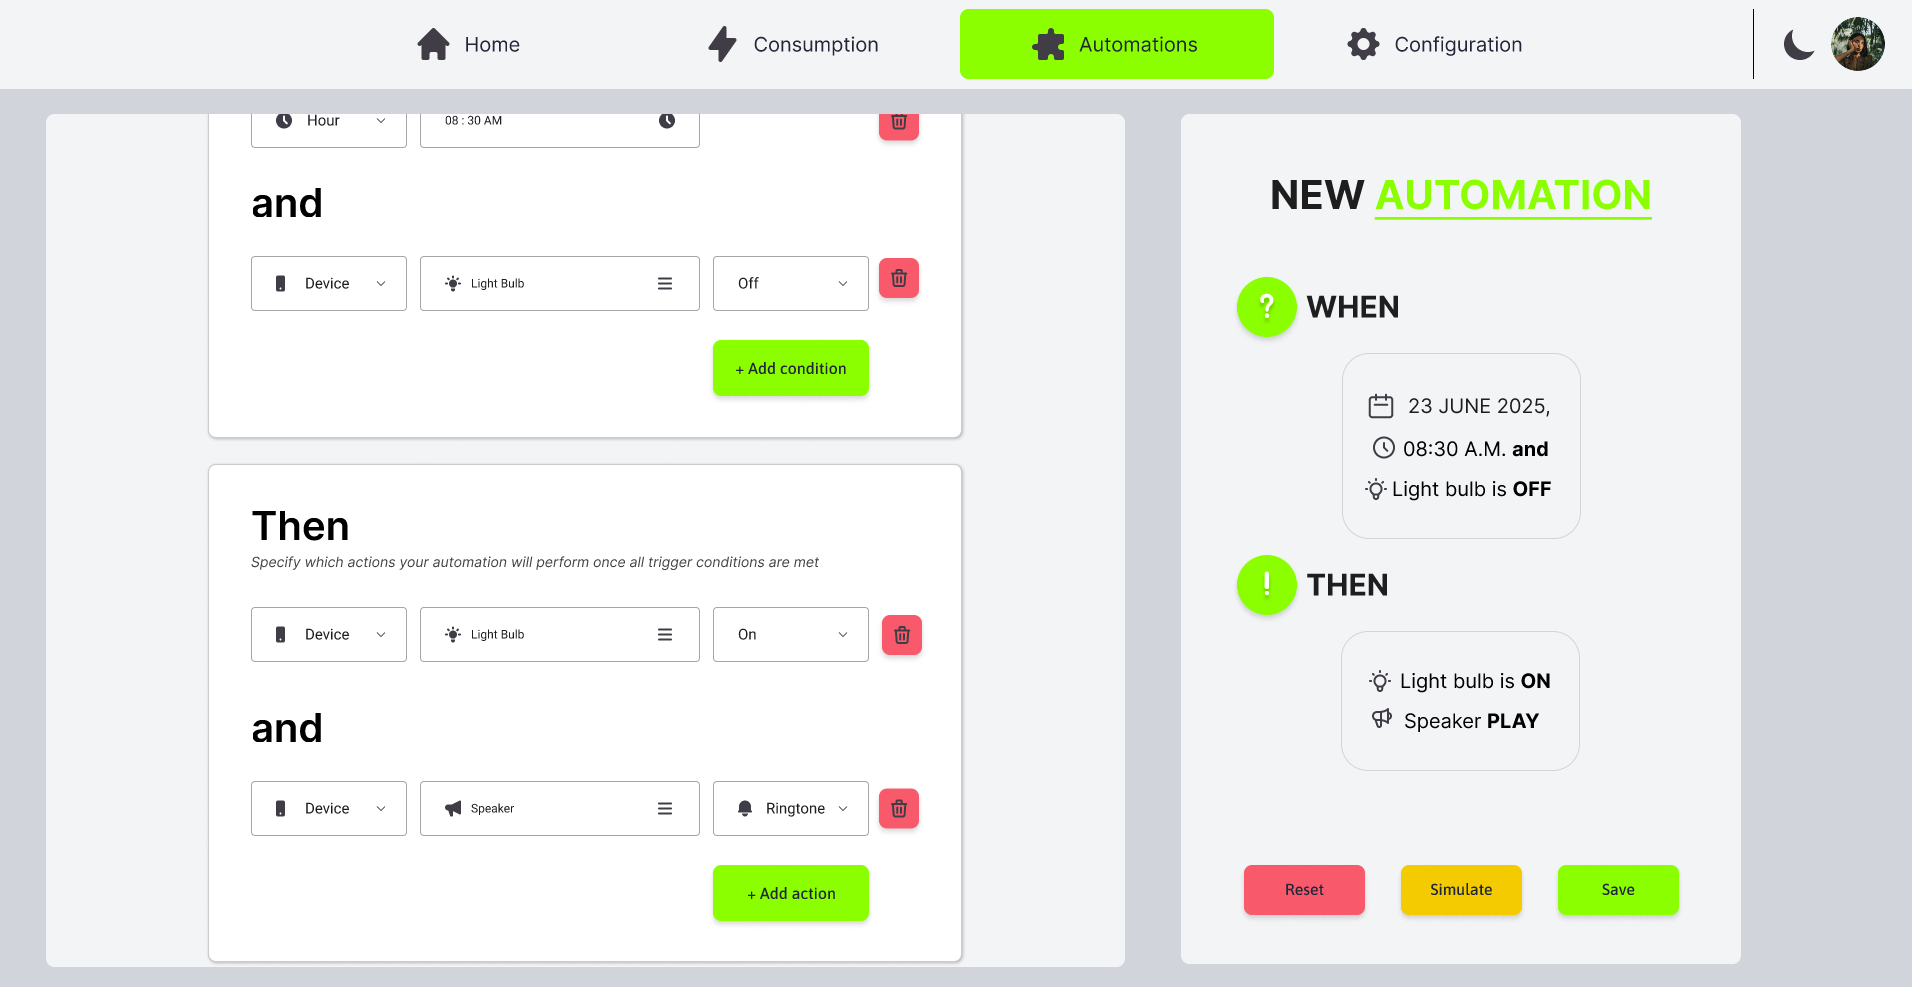
\includegraphics[width=1\linewidth]{images/Chap - 4/GOLINO/figma -UI Golino 2.png}
    \caption{Mio sviluppo: nuova interfaccia per la creazione di automazioni (parte bassa)}
    \label{fig:cap4_golino_builder_bottom}
\end{figure}

Nel dettaglio, gli elementi principali introdotti sono:
\begin{itemize}
    \item \textbf{Builder guidato a blocchi}: l'utente può aggiungere condizioni e azioni in sequenza, con pulsanti dedicati (\textit{Add condition}, \textit{Add action}).
    \item \textbf{Riepilogo immediato della regola}: il pannello laterale aggiorna in modo chiaro la logica \textit{WHEN/THEN}, riducendo ambiguità.
    \item \textbf{Controlli operativi espliciti}: i pulsanti \textit{Reset}, \textit{Simulate} e \textit{Save} rendono esplicito il passaggio tra modifica, validazione e salvataggio.
    \item \textbf{Coerenza visiva con il sistema esistente}: ho mantenuto palette, componenti e navigazione già presenti, così da non creare una rottura nell'esperienza utente.
\end{itemize}

Il pulsante \textit{Simulate} è stato pensato in coerenza con l'architettura del Capitolo~\ref{chap:digital-twin-smart-home}: prima di rendere effettiva l'automazione, la regola può essere validata dal \textit{Simulation Management Module}, mantenendo quindi la logica di prevenzione conflitti ed eccessi di consumo.

In questo modo il flusso TAP viene portato dentro la \textit{Digital Twin Interface} in maniera più completa: l'utente non si limita più a vedere automazioni esistenti, ma può creare regole nuove, verificarle e poi salvarle mantenendo un unico percorso d'uso.

\section{Aggiornamento implementativo dell'integrazione con la Smart Home}
La versione finale dell'interfaccia è stata aggiornata per operare direttamente sui dati provenienti dall'istanza reale di Home Assistant utilizzata nel caso di studio. A partire dal backup dell'abitazione intelligente, il sistema importa dispositivi, entità e automazioni esistenti, rendendoli disponibili nel Gemello Digitale attraverso le API di integrazione.

Un primo intervento ha riguardato la configurazione della planimetria e dei dispositivi. La mappa del primo piano viene utilizzata nella sezione di configurazione per collocare gli oggetti domestici nello spazio fisico; la lista laterale rende disponibili i dispositivi estratti dall'integrazione Home Assistant.

\begin{figure}[H]
    \centering
    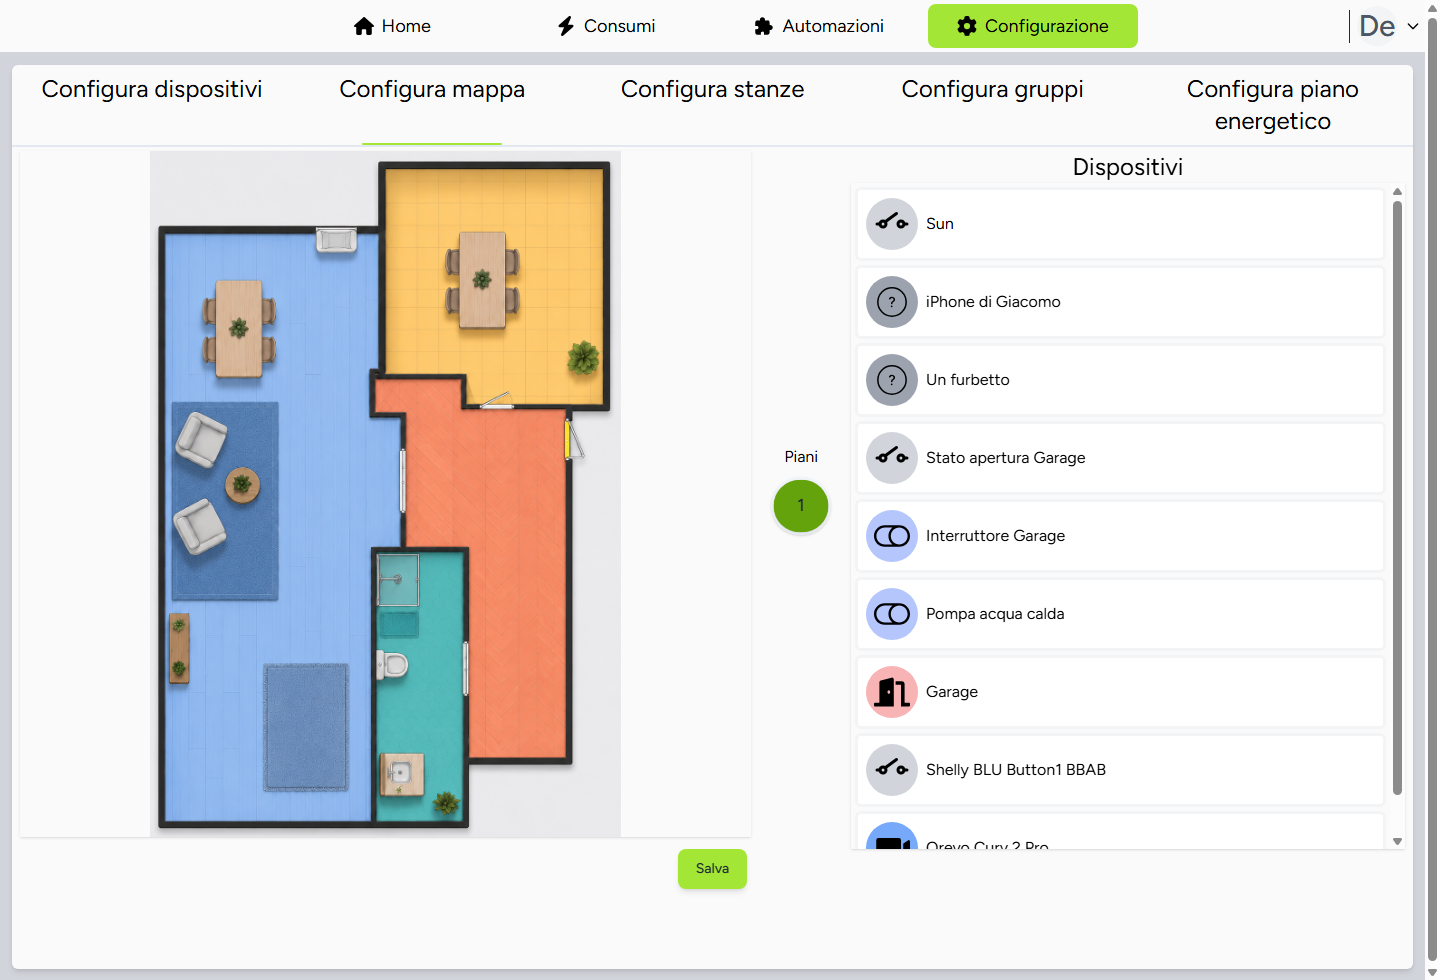
\includegraphics[width=0.95\linewidth]{images/Chap - 4/Implementation/implementation_configuration_map.png}
    \caption{Configurazione della mappa reale dell'abitazione e lista dei dispositivi importati da Home Assistant.}
    \label{fig:cap4_impl_configuration_map}
\end{figure}

Il secondo intervento ha riguardato la creazione e gestione delle automazioni. La pagina di aggiunta delle regole TAP è bilingue; il salvataggio produce una configurazione compatibile con Home Assistant e la regola è poi visibile nella pagina di elenco. Anche la cancellazione richiede una conferma esplicita e restituisce un messaggio informativo non ambiguo.

Particolare attenzione è stata dedicata al robot aspirapolvere. L'interfaccia aggrega gli script Home Assistant in un controllo orientato al dominio: l'utente sceglie il dispositivo \emph{Qrevo Curv 2 Pro}, il tipo di intervento tra \emph{Aspira}, \emph{Lava} e \emph{Aspira e lava}, quindi una o più stanze. Internamente questa scelta viene tradotta in una o più chiamate \texttt{script.turn\_on}, mantenendo la compatibilità con Home Assistant ma presentando un modello vicino all'azione domestica reale.

\begin{figure}[H]
    \centering
    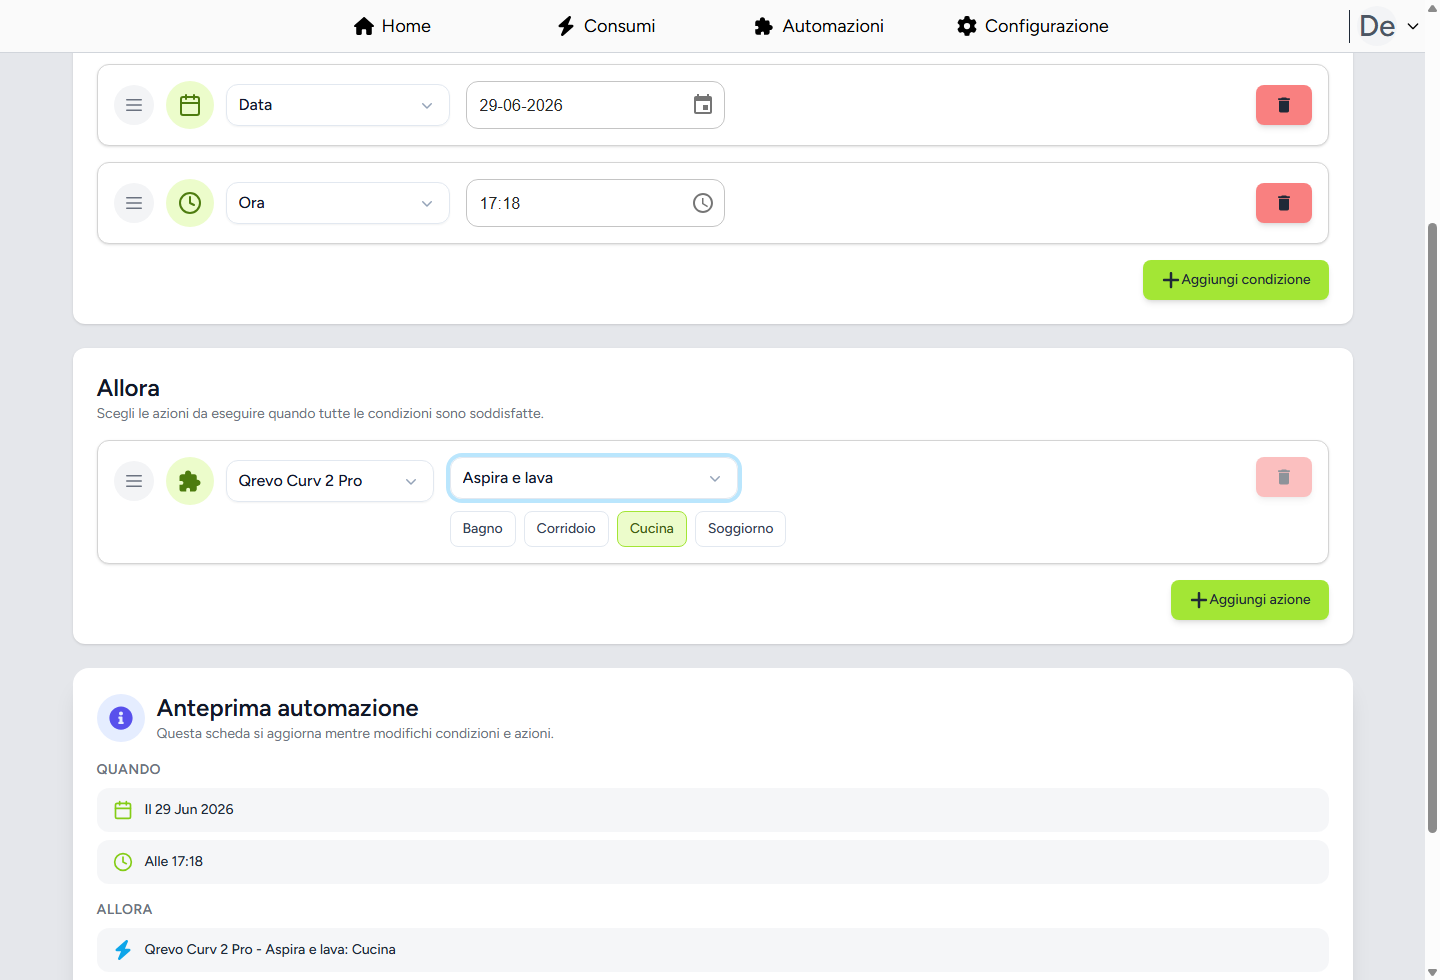
\includegraphics[width=0.95\linewidth]{images/Chap - 4/Implementation/implementation_automation_builder_robot.png}
    \caption{Creazione di un'automazione TAP con azione semantica sul robot: selezione della modalità di pulizia e delle stanze.}
    \label{fig:cap4_impl_robot_automation}
\end{figure}

La stessa schermata è stata rivista dal punto di vista responsivo: le righe dedicate a condizioni e azioni usano una griglia adattiva, evitando sovrapposizioni tra icone, selettori, pulsanti e anteprima dell'automazione anche con nomi lunghi o azioni multi-stanza.

\section{Considerazioni finali}
Il lavoro svolto in questo capitolo ha permesso di collegare in modo diretto il sistema di partenza con l'evoluzione progettata durante la tesi.

Da un lato è stato analizzato in dettaglio il prototipo iniziale, che risultava già solido per monitoraggio energetico, configurazione casa e gestione account. Dall'altro lato è stata introdotta una nuova componente centrale per la creazione guidata delle automazioni, che rappresenta il contributo principale del mio sviluppo.

Nel capitolo conclusivo verranno riprese queste scelte per discutere l'impatto complessivo sul sistema e le possibili evoluzioni future.
